\documentclass[Master,ngerman,UKenglish,eVkern,Submit]{scrbook}
%------------------------------------------------------------------------------
% This file contains a skeleton thesis for
% a Physics or Astronomy Institute in the University of Bonn

% Specify the thesis type as an option: PhD, Master, Diplom, Bachelor
% Specify the thesis stage as an option: Draft (default), Submit, Final, PILibrary

% Specify the language(s) in the class and then use babel.
% If you need more than one language, give the default language last,
% e.g. ngerman,UKenglish for a thesis in British (UK) English where you want
% to be able to set the language to German for some part of it.

%------------------------------------------------------------------------------
% Pass TeX Live version to the package
% Use command pdflatex --version to find out which version you are running
% Add option backref=false when your thesis is ready to turn off back-referencing
% in your bibliography
\usepackage[texlive=2014,backref=false]{ubonn-thesis}
% Adjustments to standard biblatex style
\usepackage{ubonn-biblatex}

% Glossary package
% \usepackage[acronym,toc,nosuper]{glossaries}
% TikZ packages and libraries
% \usepackage{tikz}
% \usepackage{tikz-3dplot}
% \usepackage{pgfplots}
% \usetikzlibrary{positioning,shapes,arrows}
% \usetikzlibrary{decorations.pathmorphing}
% \usetikzlibrary{decorations.markings}
\usepackage{overpic}
\newcommand\hmmax{0}
\newcommand\bmmax{0}
\usepackage{bm}
% \usepackage[textsize=footnotesize,english]{todonotes}
% \presetkeys{todonotes}{fancyline}{}
\usepackage{multirow}
\usepackage{thesis_defs}
\usepackage{placeins}

%------------------------------------------------------------------------------
% Instead of colouring  links, cites, table of contents etc.
% put them in a coloured box for the screen version.
% This is probably a good idea when you print your thesis.
\hypersetup{colorlinks=false,
  linkbordercolor=blue,citebordercolor=magenta,urlbordercolor=darkgreen
}

%------------------------------------------------------------------------------
% When writing your thesis it is often helpful to have the date and
% time in the output file. Comment this out for the final version.
% \ifoot[\today{} \thistime]{\today{} \thistime}

% In order to check if your labels are referenced try the refcheck package
% \usepackage{refcheck}

%------------------------------------------------------------------------------
% biblatex is included by ubonn-thesis. Look there for the settings used.
% See the options for settings that can be changed easily.
% For further changes copy the \RequirePackage[...]{biblatex} here
% and include ubonn-thesis with the option biblatex=false.

% Specify the bibliography files here and not at the end!
% Use standard_refs-bibtex if you use bibtex or bibtex8
% and standard_refs-biber  if you use biber
\addbibresource{thesis_refs.bib}
\addbibresource{../refs/standard_refs-biber.bib}

%------------------------------------------------------------------------------
% The following definitions are used to produce the title pages
% needed at various stages
\newcommand{\thesistitle}{Identification and Classification of Hadronic Tau
  Lepton Decays in the ATLAS Experiment for Run~2 of the LHC}
\newcommand*{\thesisauthor}{Christopher Deutsch}
\newcommand*{\thesistown}{Neuwied}
\renewcommand*{\InstituteName}{\PI}
\renewcommand*{\inInstitute}{\inPI}
\renewcommand*{\InstituteAddress}{\PIaddress}
% Adjust \thesisreferee...text depending on male/female referee
\newcommand*{\thesisrefereeonetext}{1.\ Gutachter}
\newcommand*{\thesisrefereeone}{Prof.\ Dr.\ Jochen Dingfelder}
\newcommand*{\thesisrefereetwotext}{2.\ Gutachter}
\newcommand*{\thesisrefereetwo}{Prof.\ Dr.\ Klaus Desch}
% Date when thesis was submitted (Master/Diplom)
% Year or Month, Year when thesis was submitted (PhD)
\newcommand*{\thesissubmit}{XX.YY.2016}
% \newcommand*{\thesissubmit}{Month 2016}
% Date of thesis examination (PhD)
\newcommand*{\thesispromotion}{XX.YY.2016}
% Month and year of the final printed version of the thesis
\newcommand*{\thesismonth}{Oktober}
\newcommand*{\thesisyear}{2017}
\newcommand*{\thesisnumber}{BONN-IR-2016-XXX}

%------------------------------------------------------------------------------
% The abstract is only needed for the printed version and should be in
% English regardless of the language of the thesis
\newcommand{\thesisabstract}{%
  \begin{otherlanguage}{UKenglish}
    This is your thesis abstract. It may be in a language that is
    different from the rest of your thesis.
  \end{otherlanguage}
}

%------------------------------------------------------------------------------
% \includeonly can be used to select which chapters you want to process
% A simple \include command just inserts a \clearpage before and after the file
% Note that \includeonly can be quite picky! Do not forget to put a
% comma after the filename, otherwise it will simply be ignored!
% \includeonly{%
%   thesis_intro,
%   thesis_appendix,
%   thesis_acknowledge
% }

%------------------------------------------------------------------------------
% Give a list of directories where figures can be found. Do not leave
% any spaces in the list and end the directory name with a /
\graphicspath{%
  {../figs/}%
  {../figs/cover/}%
  {../figs/graphics/}%
  {../feynmf/}%
}

%------------------------------------------------------------------------------
% Make a glossary and a list of acronyms
% \makeglossaries

% Glossary entries
% \input{thesis_glossary}

% Draft version - add the word DRAFT on the cover pages
\ifthenelse{\equal{\ThesisVersion}{Draft}}{%
  \usepackage{background}
  \ifthenelse{\texlive < 2013}{%
    \SetBgContents{DRAFT}
    \SetBgColor{blue!30}
  }{%
    \backgroundsetup{contents=DRAFT, color=blue!30}
  }
}

% ------------------------------------------------------------------------------
% My packages
\usepackage{listings}

%------------------------------------------------------------------------------
\begin{document}

% Cover page of thesis - this is only needed for the printed final
% version to be submitted to the department library
% Do not use this page for thesis submission to the Prüfungsamt or Promotionsbüro!
\ifthenelse{\equal{\ThesisVersion}{PILibrary}}{%
  \typeout{Document \jobname, Info: PI library version of thesis}
  \input{../cover/\ThesisType_Cover}
}{}

% Start counting pages from the title page
\frontmatter
% Dedication has to come before \maketitle
% \dedication{For ...}

% Select the correct title page(s)
\ifthenelse{\equal{\ThesisType}{Unknown}}{%
  \typeout{Document \jobname, Error: Unknown thesis type - no title page printed}
}{%
  % Bachelor thesis only has one title page
  \ifthenelse{\equal{\ThesisType}{Bachelor}}{%
    \typeout{Document \jobname, Info: Bachelor thesis}
    \input{../cover/\ThesisType_Title}
  }{%
    \ifthenelse{\equal{\ThesisVersion}{Final} \OR \equal{\ThesisVersion}{PILibrary}}{%
      % Final and PI library versions
      \typeout{Document \jobname, Info: Final version of a \ThesisType  thesis}
      \input{../cover/\ThesisType_Final_Title}
    }{% Submission and draft versions
      \input{../cover/\ThesisType_Submit_Title}
      \typeout{Document \jobname, Info: Draft/submission version of a \ThesisType  thesis}
    }
  }
}

\pagestyle{scrplain}

%------------------------------------------------------------------------------
% You can add your acknowledgements here - don't forget to also add
% them to \includeonly above
\tableofcontents

\mainmatter
\pagestyle{scrheadings}

% Turn off DRAFT for the following pages
\ifthenelse{\equal{\ThesisVersion}{Draft}}{%
  \ifthenelse{\texlive < 2013}{%
    \SetBgContents{}
  }{%
    \backgroundsetup{contents={}}
  }
}{}

%------------------------------------------------------------------------------
% Add your chapters here - don't forget to also add them to \includeonly above
\chapter{Introduction}
\label{sec:intro}

Outline of the thesis:

\section{Introduction}

\begin{itemize}
\item LHC \& Experiments
  \begin{itemize}
  \item Discoveries / Measurements

  \item Past: Run-I, Present: Run-II, Future: HL-LHC \& Challenges
  \end{itemize}

\item $\tau$-Leptons
  \begin{itemize}
  \item Importance (Fermionic coupling of Higgs, Higgs CP, Exotics $Z^\prime$,
    $W^\prime$, Heavy Higgs, SUSY)
  \item $\tau$-decay (hadronic branching fraction, decay modes)
  \item Jets faking taus (necessity of identification algorithms)
  \item Classification of $\tau$ decay modes (motivation)
  \end{itemize}

\item Overview of the thesis structure (one bullet point per chapter).
\end{itemize}

\section{Theoretical Background}

\begin{itemize}
\item The Standard Model
  \begin{itemize}
  \item Features \& Successes

  \item Challenges (neutrino masses, dark matter, matter-antimatter asymmetry,
    gravitation, number of parameters, hierarchy problem, \ldots)

  \item Beyond the Standard Model (SUSY -- preferred coupling to down-type
    fermions for large $\tan\beta$ \textrightarrow $\tau$-leptons)
  \end{itemize}

\item Weak Interaction
\begin{itemize}
\item ?
\end{itemize}

\item Strong Interaction
\begin{itemize}
\item ?
\item Confinement \& Hadronization
\item Quark \& Gluon initiated jets
\end{itemize}

\item $\tau$-Leptons
\begin{itemize}
\item Discovery

\item Properties (mass \textrightarrow lep \& had, mean life time
  \textrightarrow no direct detection)

\item Hadronically Decaying $\tau$-Leptons
  \begin{itemize}
  \item Feynman Diagram, Decay Modes (interm. resonances) \& Branching Ratios
  \item Detector signature ($\pi^0$ ($\gamma \gamma$ / $\mathrm{e}^+
    \mathrm{e}^- \gamma$), $\pi^\pm$ ($\mathrm{K}^\pm$), $\nu_\tau$)
  \item Jets faking taus
  \item
  \end{itemize}

\item $\tau$ Physics
  \begin{itemize}
  \item $\mathrm{Z} \rightarrow \tau \tau$ (background for H$\tau \tau$ and
    useful for performance measurements using tag-and-probe -- semileptonic
    decays)

  \item $\mathrm{H} \rightarrow \tau \tau$ (one of two channels to measure
    the fermionic coupling -- $b \bar{b}$ plagued by multijet background,
    Higgs CP)

  \item MSSM Higgs (potentially high branching fraction to $\tau$-leptons)

  \item $\mathrm{Z}^\prime$ could preferentially decay into third-generation
    fermions (lepton universality not required).

  \item $\mathrm{W}^\prime$ models with preferential coupling to third-gen.
  \end{itemize}
\end{itemize}

\end{itemize}

\section{Machine Learning (worthy of own chapter?)}

\begin{itemize}
\item Own chapter describing the machine learning methods used or include into
  \textit{Theoretical Background}? Alternatively include theory section where
  needed (e.g. have one for the BDT-based studies explaining BDTs [short] and
  one for the RNN studies [longer]).

\item Boosted Decision Trees
  \begin{itemize}
  \item Boosting: Adaptive Boosting $\alpha$, Gradient Boosting $\eta$
  \item Node splitting: Gini Index
  \item Hyperparameters: $N_\mathrm{Trees}$, $d_\mathrm{Tree}$,
  \end{itemize}

\item Neural Networks
  \begin{itemize}
  \item Basics -- focussed on forward pass (Densely connected layers, Activation)
  \item Training -- Weight initialization, Loss functions, Minibatch Gradient
    Descent, Cross-Validation (training, validation, test split)
  \item Recurrent Neural Networks (RNN Equations, Vanishing Gradient Problem,
    Physics Motivation)
  \item Long Short-Term Memory \cite{lstm} (LSTM Equations)
  \item Technical setup (Keras, theano)
  \end{itemize}
\end{itemize}

\section{ATLAS Experiment and the LHC}

\begin{itemize}
\item LHC (brief)

\item ATLAS
  \begin{itemize}
  \item Overview (Design goals) \\
    brief: Beam Line, Inner Detector \& Solenoid, Calorimeter, Muon System \&
    Toroid, Trigger

  \item Nomenclature (Coordinate system, Pseudorapidity, $\Delta R$)

  \item Inner detector / Tracker
    \begin{itemize}
    \item Pixel, IBL
    \item SCT
    \item TRT
    \item  Transverse Momentum Resolution, Vertex \& Secondary Vertex
      reconstruction, Impact Parameter Resolution, $\eta$-Coverage
    \end{itemize}

  \item Calorimeter
    \begin{itemize}
    \item Presampler, LAr (EM1 - EM3), Had (Tile, LAr)
    \item $\eta$-Coverage, Thickness $X_0$ / $\lambda$, Energy Resolution
      vs. $E$
    \item Topoclusters \& Cluster moments
    \end{itemize}

  \end{itemize}
\end{itemize}

\section{Reconstruction of Hadronically Decaying $\tau$-Leptons at ATLAS}

\begin{itemize}
\item anti-$k_\mathrm{t}$ Jets $R = 0.4$
\item Track Selection \& TJVA
\item MVA tracking
\item Energy \& Calibration
\item Tau-ID (does not fit in here)
\item Substructure Reconstruction (Decay Mode Classification)
\end{itemize}

\section{Identification of Hadronically Decaying $\tau$-Leptons (BDT part)}

\begin{itemize}
\item Features of hadronically decaying $\tau$-leptons vs. Quark/Gluon
  initiated jets

\item Samples
  \begin{itemize}
  \item Gammatautau (Polarization), Dijet JZ1W - JZ6W
  \item Reweighting
  \item Baseline selection ($\eta$, $p_\mathrm{T}$, truth-matching)
  \end{itemize}

\item BDT-based Studies
  \begin{itemize}
  \item Previous setup (incl. explanation \& plots of input variables)
  \item Hyperparameter optimization
    \begin{itemize}
    \item AdaBoost \textrightarrow GradBoost
    \item Grid Search
    \item XGBoost (?)
    \end{itemize}
  \item Variable correlations, importance (dropped variables) \& dependence with
    $p_\mathrm{T}$ (2D Hist), Variable Transformations (instead of cutting out
    outliers), Partial Dependence
  \item Working points (Gammatautau -- Ztautau)
  \item Performance on simulated data
  \item Impact of Quark / Gluon initiated jets on Tau-ID
  \end{itemize}

\end{itemize}

\section{Identification of Hadronically Decaying $\tau$-Leptons (NN-part)}

\begin{itemize}
\item Neural Network-based Studies
  \begin{itemize}
  \item MLP Tau-ID
  \item Track-RNN
    \begin{itemize}
    \item Architecture
    \item Input variables \& correlation with true class labels
    \item Validation loss vs. number of tracks
    \end{itemize}
  \item Cluster-RNN \& Potential rate-reduction at HLT
    \begin{itemize}
    \item Validation loss vs. number of clusters
    \item Input variables \& correlation with true class labels
    \end{itemize}
  \item Combined-RNN
  \end{itemize}
\end{itemize}

\section{Decay Mode Classification for Hadronically Decaying}

\begin{itemize}
\item Signature of the decay modes
\item Explain PFO
\item RNN
  \begin{itemize}
  \item Only PFOs
  \item PFOs + Extras
  \end{itemize}
\end{itemize}

\section{Conclusion}

\begin{itemize}
\item
\end{itemize}

\section{Appendix}

\begin{itemize}
\item MC Samples (Preprod, MC16A)
\end{itemize}

%%% Local Variables:
%%% mode: latex
%%% TeX-master: "mythesis"
%%% End:

% ~ 6 pages
\chapter{Theoretical Background}
\label{sec:theory}

In this chapter the theoretical background for the studies in this thesis is
provided. First the Standard Model of particle physics is introduced and its
problems discussed. Then physics of tau leptons is discussed with a focus on
hadronic decays of the tau lepton.

\section{The Standard Model of Particle Physics}

The Standard Model of particle physics describes the current understanding of
elementary particles and interactions between them. The Standard Model has been
extensively probed since its origin and shows excellent agreement with
experimental results. However, it does not offer a full description of particle
physics as it does not explain interactions of massive particles via gravity.

In Figure~\ref{fig:sm_particles} the elementary particles of the SM are shown.
They can be divided into the fermions consisting of particles with spin-half and
gauge with spin-1. In 2012 the ATLAS and CMS experiment at the Large Hadron
Collider discovered a new scalar boson with a mass
of~$m_\text{H} \approx \SI{125}{\GeV}$~\cite{higgs_atlas, higgs_cms}, which is
called the Higgs boson (SM like).

\begin{figure}[htb]
  \centering
  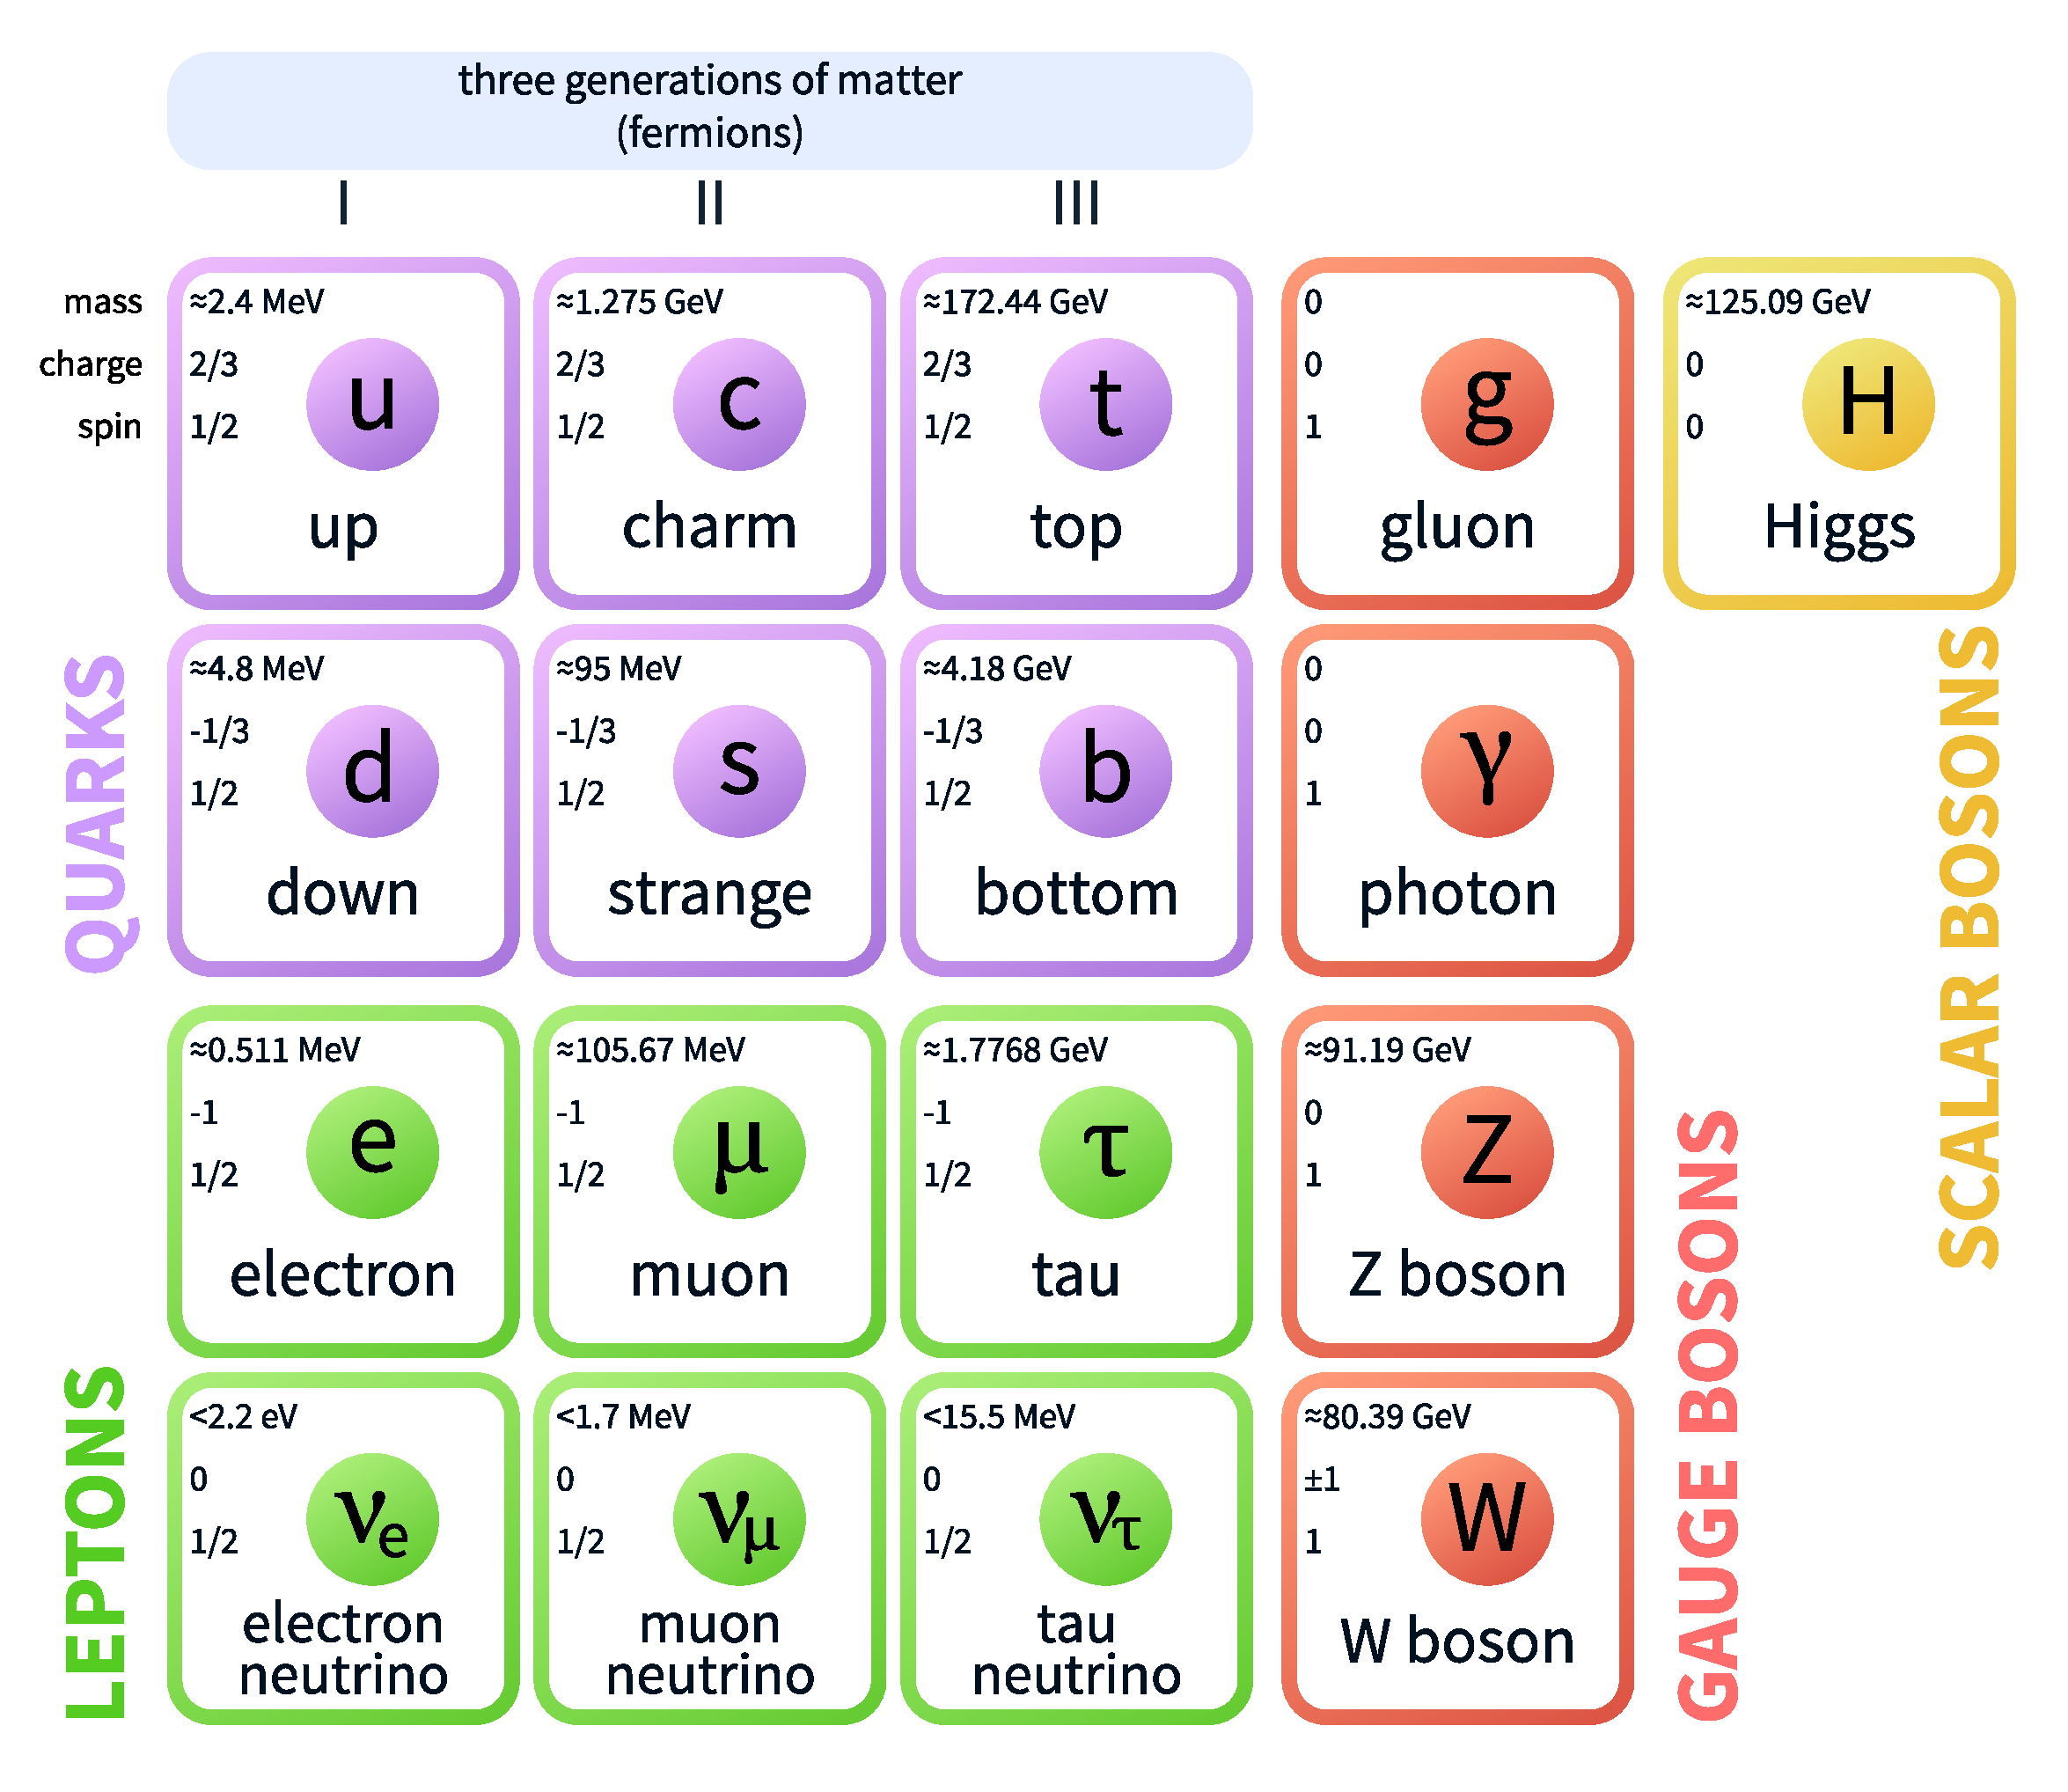
\includegraphics[width=0.7\textwidth]{./figures/theory/sm_particles.pdf}
  \caption{Particles of the Standard Model. Image modified from
    Ref.~\cite{sm_wiki}.}
  \label{fig:sm_particles}
\end{figure}

In the following the elementary particles and their interactions are described.
The fermions of the Standard Model form the observable matter. The dynamics of
fermions are described by the Dirac equation, while interactions between them
are mediated by the gauge bosons. The nature of these interactions is described
by quantum field theories and the local gauge principle. The fermions are
divided into up- and down-type quarks with a charge of~$\frac{2}{3}$
and~$-\frac{1}{3}$, respectively and leptons consisting of the charged leptons
and the neutrinos. The fermions are divided into three generations with
identical properties with the exception of their mass. The first generation
consisting of the electron, electron neutrino, up- and down-quark makes up most
of the matter in the low-energy universe. The quarks of the second and third
generation are produced in high-energy particle collisions. Each fermion has a
corresponding antiparticle with the same mass but with inverted additive quantum
numbers including the electric charge.

The strong interaction between quarks is described by quantum chromodynamics.
The exchange particle of the strong force is the massless gluon, which couples
to the so called color charge. The quarks as well as the gluons carry color
charge allowing $qqg$-vertices as well as gluon self-coupling in triple and
quartic gluon vertices. Experimentally, free quarks are not observed but only
color-neutral bound states called hadrons. This is known as colour confinement
and leads to the formation of collimated jets of hadrons in processes creating
high-energy quarks or gluons.\todo{Ben -- write sth.\ about the hadronisation
  process}

The electromagnetic interaction between particles carrying electric charge is
described by quantum electrodynamics. The mediating gauge boson is the massless
photon, which couples to charged particles including quarks, charged leptons and
the $W^\pm$~boson.

The weak interaction is mediated by the massive $Z^0$ and $W^\pm$~bosons, which
couple to the weak charges carried by all fermions. Additionally, couplings
between the weak bosons itself are allowed. The weak interaction violates
$\mathcal{P}$ and $\mathcal{CP}$ symmetry. The weak charged-current interaction
is mediated by the $W^\pm$~boson and couples to chiral left-handed particles and
chiral right-handed antiparticles. The weak charged-current allows flavour
changes in the quark sector. In contrast to this, the weak neutral-current
interaction mediated by the $Z^0$~boson does not allow flavour changes. The
$Z^0$ couples to both left- and right-handed particles although with different
strength.

The electromagnetic and weak interactions are unified in the electroweak theory
developed by Glashow, Salam and Weinberg~\cite{glashow, salam, weinberg}. The
local gauge symmetry~$\mathrm{SU}(2)_\text{L}$ generating the weak
charged-current interaction and the $W^+$, $W^-$ boson fields as well as a
neutral field $W^{(3)}$ coupling to chiral left-handed particles. The
electroweak unification introduces a $\mathrm{U}(1)_Y$, where~$Y = 2 (Q - T_3)$
is the weak hypercharge depending on the electric charge~$Q$ and the third
component of the weak isospin~$T_3$. The~$\mathrm{U}(1)_Y$ symmetry generates a
neutral field~$B$ that mixes with~$W^{(3)}$ giving rise to the photon and $Z^0$
boson fields, thus combining the weak and the electromagnetic interaction.

The non-vanishing masses of the $W^\pm$ and $Z^0$ bosons break the local gauge
invariance of the electroweak theory when introducing a mass term into the
Lagrangian. To maintain the gauge principle a different approach called the
Higgs mechanism~\cite{englert_brout, higgs} is introduced so that the weak
bosons can acquire their mass in a process called \emph{spontaneous symmetry
  breaking}. For this a doublet of complex scalar fields with non-vanishing
vacuum expectation value is introduced. This breaks the symmetry of the
Lagrangian and introduces four degrees of freedom. Three are absorbed into the
$W^+$, $W^-$ and $Z^0$ bosons giving them mass. The remaining neutral and scalar
component becomes the physical Higgs boson. The Higgs mechanism is also used to
generate masses of the fermions, however neutrinos are assumed to be massless in
the Standard Model.

\subsection{Problems of the Standard Model}

The Standard Model predicts and has been extensively tested. However, some
phenomena remain unexplained in the Standard Model:
\begin{description}
\item[Gravity] Currently, no complete and consistent quantum field theory of
  gravity exists. Therefore, the Standard Model cannot describe the
  gravitational interaction between massive particles.

\item[Dark matter] The Standard Model does not provide a weakly interacting
  massive particle that explains both the observed gravitational interaction of
  dark matter as well as the large-scale structure of the observable Universe.

\item[Origin of neutrino masses] The discovery of neutrino
  oscillations~\cite{superk_neutrino, sno_neutrino_1, sno_neutrino_2} show that
  neutrinos have mass. The origin of this mass is not determined in the Standard
  Model. It can be generated using the Higgs mechanism making neutrinos Dirac
  particles. Another possibility is neutrinos being Majorana particles, in which
  case the seesaw mechanism could explain the experimentally observed mass scale
  of neutrinos.

\item[Matter--antimatter asymmetry] The baryon number and $\mathcal{CP}$
  violation required by the Sakharov conditions~\cite{sakharov} to explain the
  observed matter--antimatter asymmetry, cannot be provided in the Standard
  Model.

\item[Hierarchy problem] The Higgs boson mass is modified by radiative
  corrections due to fermionic and bosonic loops in the Higgs
  propagator~\cite{bettini}. At high energy scales the Higgs mass would be
  large, requiring fine-tuning of the contributions to the Higgs mass to keep it
  at the electroweak scale~\cite{thomson}. Supersymmetry offers a solution to
  this problem, cancelling the corrections.

\item[Unification of the forces] The couplings of the three interactions
  described in the Standard Model are of the same order of magnitude at the
  electoweak energy scale. They might converge at even higher energies,
  suggesting that the Standard Model is only a low-energy manifestation of a
  unified theory~\cite{thomson}.

\item[Number of parameters] A total of 26 free parameters consisting of 12
  fermion masses, 3 coupling constants, the vacuum expectation value of the
  Higgs field and mass of the Higgs boson, 6 mixing angles and 2 phases in the
  PMNS and CKM matrix and potentially a $\mathcal{CP}$~violating phase of the
  strong interaction, are needed to describe the Standard Model~\cite{thomson}.
  The large number of parameters is sometimes viewed as inelegant for describing
  a fundamental theory.
\end{description}
Explanation for these issues need to extend the Standard Model or introduce new
theories beyond the Standard Model, e.g.\ Supersymmetry or Grand Unified
Theories.

\section{Tau Leptons}

The tau lepton was discovered in 1975 by Martin Lewis Perl \textit{et al.} with
the LBL detector at the SPEAR electron--position collider at SLAC~\cite{perl}.
With a mass of~\SI{1776.86 +- 0.12}{\MeV} it is the heaviest lepton in the
Standard Model and has a mean lifetime of \SI{290.3 +-
  0.5}{\femto\second}~\cite{pdg}.

\subsection{Tau Decay}

The tau lepton decays via the weak charged-current interaction shown in
Figure~\ref{fig:tau_feynman}. Due to the unit charge of the tau lepton, the
decay products of a tau decay always contains an odd number of charged
particles. Tau decays with $N$ charged daughter particles are called $N$-prong
decays. With a branching fraction of more than \SI{99}{\percent}, the vast
majority of tau decays are 1- or 3-prong. The tau lepton is more than twelve
times heavier than pions and therefore can decay leptonically as well as
hadronically. The leptonic modes~$\tau^- \to e^- \bar{\nu}_e \nu_\tau$
and~$\tau^- \to \mu^- \bar{\nu}_\mu \nu_\tau$ make up about \SI{35}{\percent} of
tau decays (cf.\ Figure~\ref{fig:tau_branching_ratios}), with almost equal
branching fractions to $e^- \bar{\nu}_e \nu_\tau$ and
$\mu^- \bar{\nu}_\mu \nu_\tau$. A large fraction of decays proceed via hadronic
decay modes producing charged and neutral mesons and a tau neutrino. Mostly
pions are created in hadronic tau decays, as the production of strange quarks is
suppressed by a factor
of~$\sin^2\theta_\text{c} / \cos^2\theta_\text{c} \approx \frac{1}{20}$
(neglecting phase space difference), where $\theta_\text{c}$ is the Cabibbo
angle. Therefore, kaons are rarely produced in hadronic tau decays.

Charged pions are stable

Neutral pions immediately decay into two photons with a branching ratio of
\SI{}{\percent}~\cite{pdg}

Focus on hadronic decays. Why?


- Possible decays and intermediate resonances:

Two or three pion modes mainly through intermediate $\rho$ or $a_1$
  resonances

- Introduce \tauhad

- Define what 'visible' means (Missing tau neutrino) and \tauhadvis


The tau lepton is the heaviest lepton in the Standard Model and an important
probe of physics at high energy scales, such as Higgs physics and physics beyond
the Standard Model. Hadronic decays make up approximately two-thirds of the
total branching ratio of tau decays and play an important part in the physics
programme of the ATLAS experiment.


\begin{itemize}
\item Charged pion 'stable' and showers in the HCAL
\item Neutral pion decays immediately into two photons which shower in the ECAL.
  Created photons often convert into an electron positron pair in the presence
  of material
\end{itemize}




\begin{figure}[htb]
  \begin{subfigure}[b]{0.47\textwidth}
    \centering
    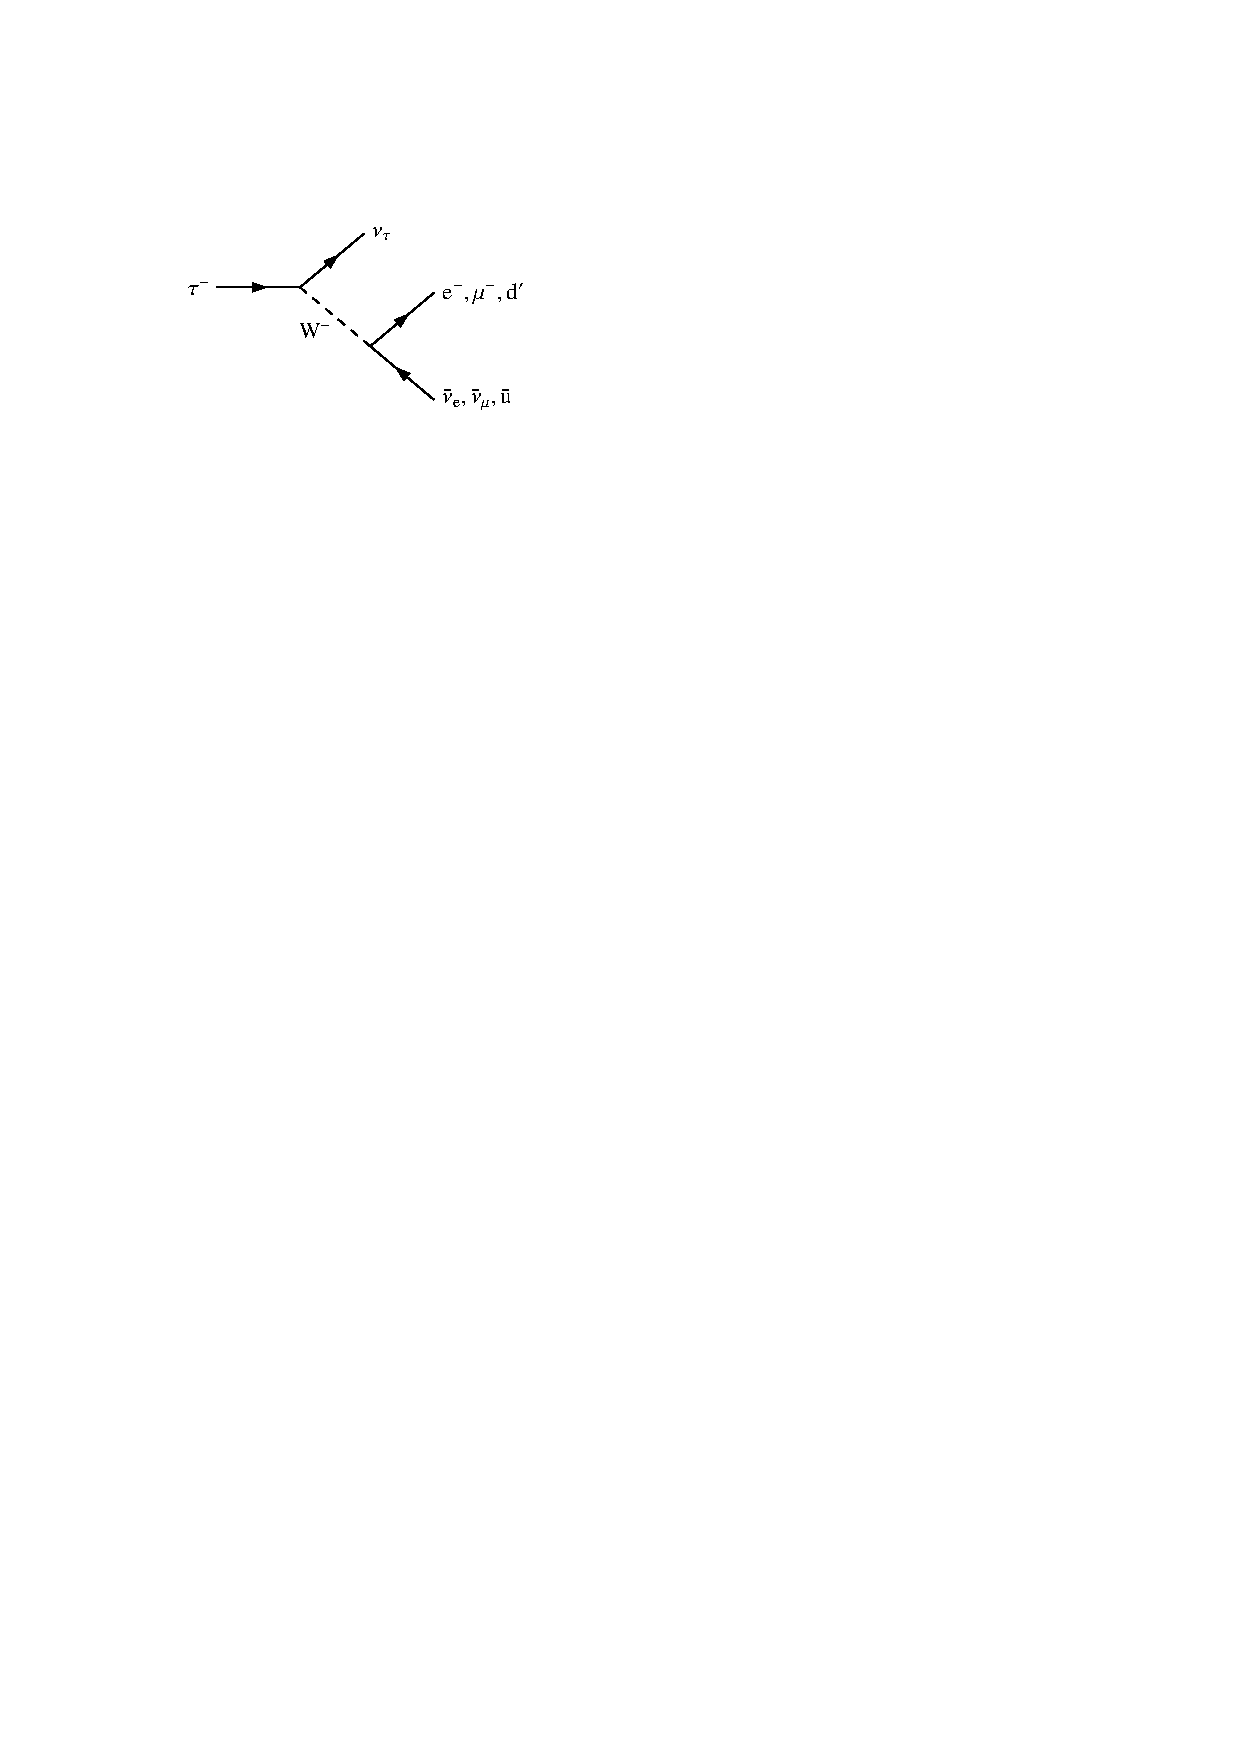
\includegraphics{./figures/theory/tau_decay_feynman.pdf}
    \vspace*{2em}
    \caption{Feynman diagram of the tau decay via the weak interaction. The
      $d^\prime$ is the weak eigenstate mixing the mass eigenstates of the $d$
      and $s$ quark.}
    \label{fig:tau_feynman}
  \end{subfigure}\hfill
  \begin{subfigure}[b]{0.47\textwidth}
    \centering
    \begin{overpic}[scale=0.9]{./figures/theory/tau_branching_pie_chart.pdf}
      \put (33.5, 83) {$\pi^- \nu_\tau$}
      \put (-2, 45) {$\pi^- \pi^0 \nu_\tau$}
      \put (19, 7.5) {$\pi^- 2 \pi^0 \nu_\tau$}
      \put (44, 2) {$2 \pi^- \pi^+ \nu_\tau$}
      \put (69, 6) {$2 \pi^- \pi^+ \pi^0 \nu_\tau$}
      \put (80, 15) {other}
    \end{overpic}
    \caption{Tau lepton branching ratios~\cite{pdg}. Adapted from
      Ref.~\cite{ikai_trigger}.}
    \label{fig:tau_branching_ratios}
  \end{subfigure}
  \caption{Weak decay and branching ratios of the tau lepton.}
\end{figure}




      % Feynman Diagram. Strangeness production is Cabibbo suppressed by a factor
      % of
      % $\sin^2\theta_\mathrm{c} / \cos^2\theta_\mathrm{c} \approx \frac{1}{20}$.
      % Ignoring phase space considerations the tau decays to $\frac{1}{5}$ into
      % electron or muon and corresponding antineutrino or into a down anti-up
      % quark pair (3 colours).



\subsection{Features of Hadronically Decaying Tau Leptons}
\label{sec:features_tau_decay}

\todo[inline]{Ignore non 1- and 3-prong modes.}

\todo[inline]{Signature of the decay modes}

\todo[inline]{Leptonic decays of the tau are identified using the electron/muon
  identification.}

\todo[inline]{Quark-like jets are on average more collimated and have fewer
  tracks and thus the discrimination from \tauhadvis is less effective than for
  gluon-like jets. Due to higher effective colour charge for gluons.}


Features of hadronically decaying $\tau$-leptons vs. Quark/Gluon initiated jets:
\begin{itemize}
\item Low multiplicity (QCD jets usually have a lot of tracks)
\item Isolated tracks and narrow showers
\item Measurable decay length with proper lifetime of
  $\tau = \SI{290.3 +- 0.5}{\femto\second}$ \cite{pdg} and following from that
  $c \tau = \SI{87.0 +- 0.2}{\micro\metre}$ with $\beta \gamma = 10$ which
  corresponds to a roughly \SI{18}{\giga\electronvolt} tau the mean decay length
  is of the order of a millimetre and allows secondary vertex reconstruction or
  employing the impact parameter for 1-prong taus (sub-millimetre resolution).
\item Invariant mass bounds for decay products
\item $\pi^0$ content???
\item Cross section plot multijet (large cross section) vs.
  electroweak interaction (small)
\item Detector signature ($\pi^0$ ($\gamma \gamma$ / $\mathrm{e}^+
  \mathrm{e}^- \gamma$), $\pi^\pm$ ($\mathrm{K}^\pm$), $\nu_\tau$,
  conversions)
\item Jets faking taus
\item \url{http://www.hep.ph.ic.ac.uk/~wstirlin/plots/plots.html}
\item Quark vs Gluon jets: \url{http://jets.physics.harvard.edu/qvg/}
  Because of different colour interaction and hadronization, gluon jets are
  wider, with higher multiplicity and have a more uniform energy
  fragmentation, while quark jets are more likely to produce narrow jets with
  hard constituents that carry a significant fraction of the energy.
\end{itemize}

Most common high-energy process at the LHC: Production of dijet-events (back to
back in the transverse plane). A lot of QCD diagrams contribute to the dijet
cross-section (qq \textrightarrow qq, qq \textrightarrow gg, gg \textrightarrow
qq, qg \textrightarrow gq, gg \textrightarrow gg, etc.). Dijet cross-section
peaked at low $p_{\text{T}}$.

\subsection{Tau Lepton Physics at the LHC}

Focus on $H \to \tauhad \tauhad$ (Also mention $\mathcal{CP}$ measurement) and
$Z^\prime$ analyses.

Zprime conf note
https://atlas.web.cern.ch/Atlas/GROUPS/PHYSICS/CONFNOTES/ATLAS-CONF-2017-050/



To investigate mass generation mechanism for fermions as implemented in the
Standard Model, it is of prime importance to demonstrate direct coupling of the
Higgs boson to fermions and the proportionality of its strength to mass.

Only channel $H \to \tau \tau$ and $h \to b \bar{b}$ but $b \bar{b}$
difficult due to high background. $\tau\tau$ favourable sensitivity.

\begin{figure}[htbp]
  \begin{subfigure}[t]{0.48\textwidth}
    \centering
    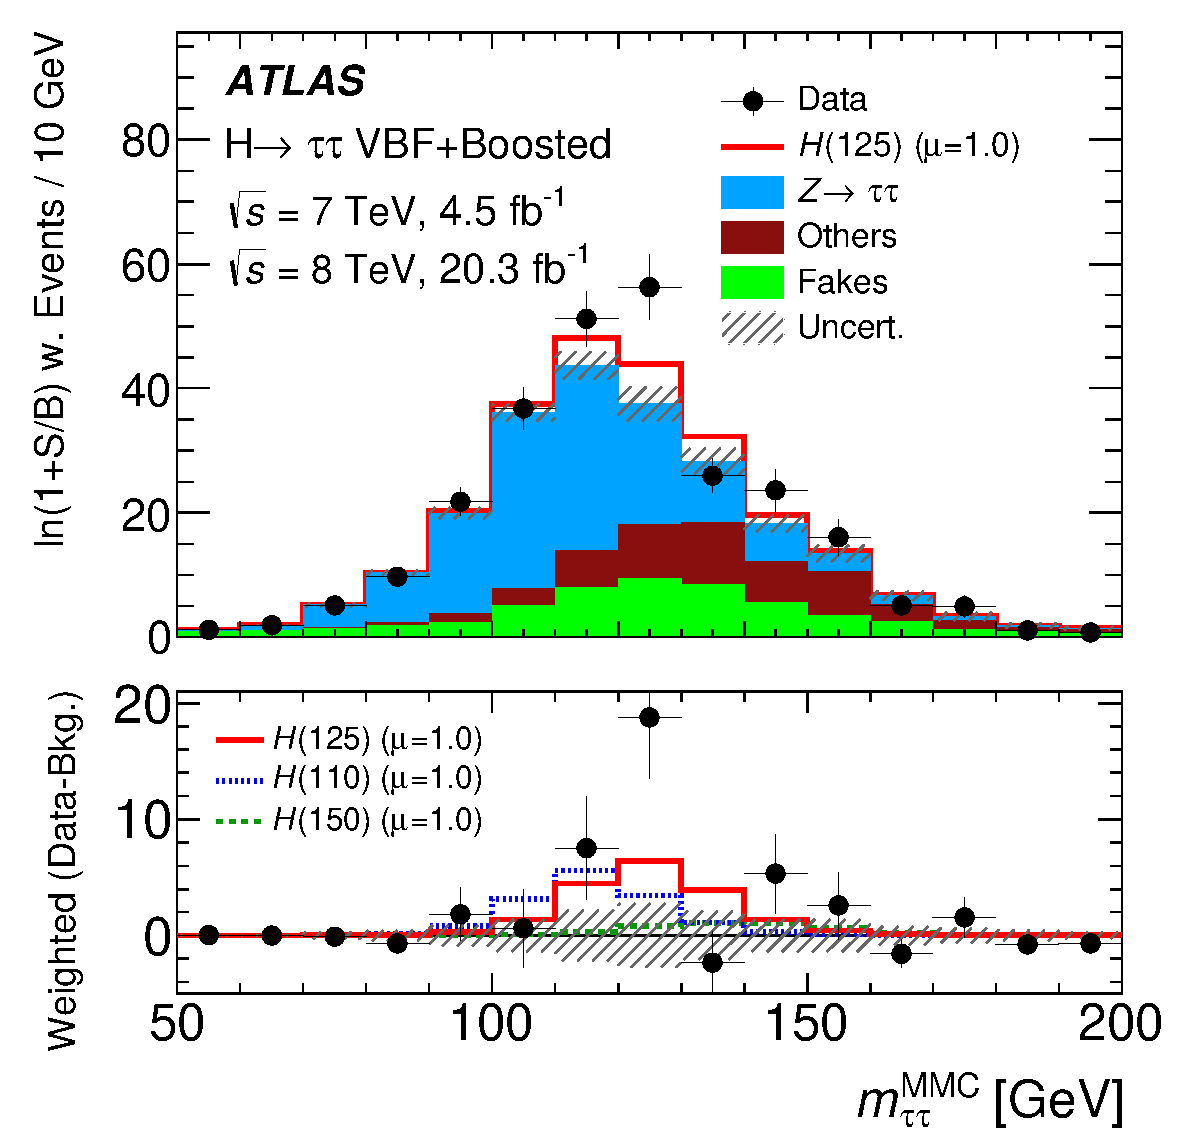
\includegraphics[width=1.0\textwidth]{./figures/theory/htautau_mass.pdf}
    \subcaption{$H \to \tau\tau$~\cite{higgs_tautau}}
  \end{subfigure}\hfill
  \begin{subfigure}[t]{0.48\textwidth}
    \centering
    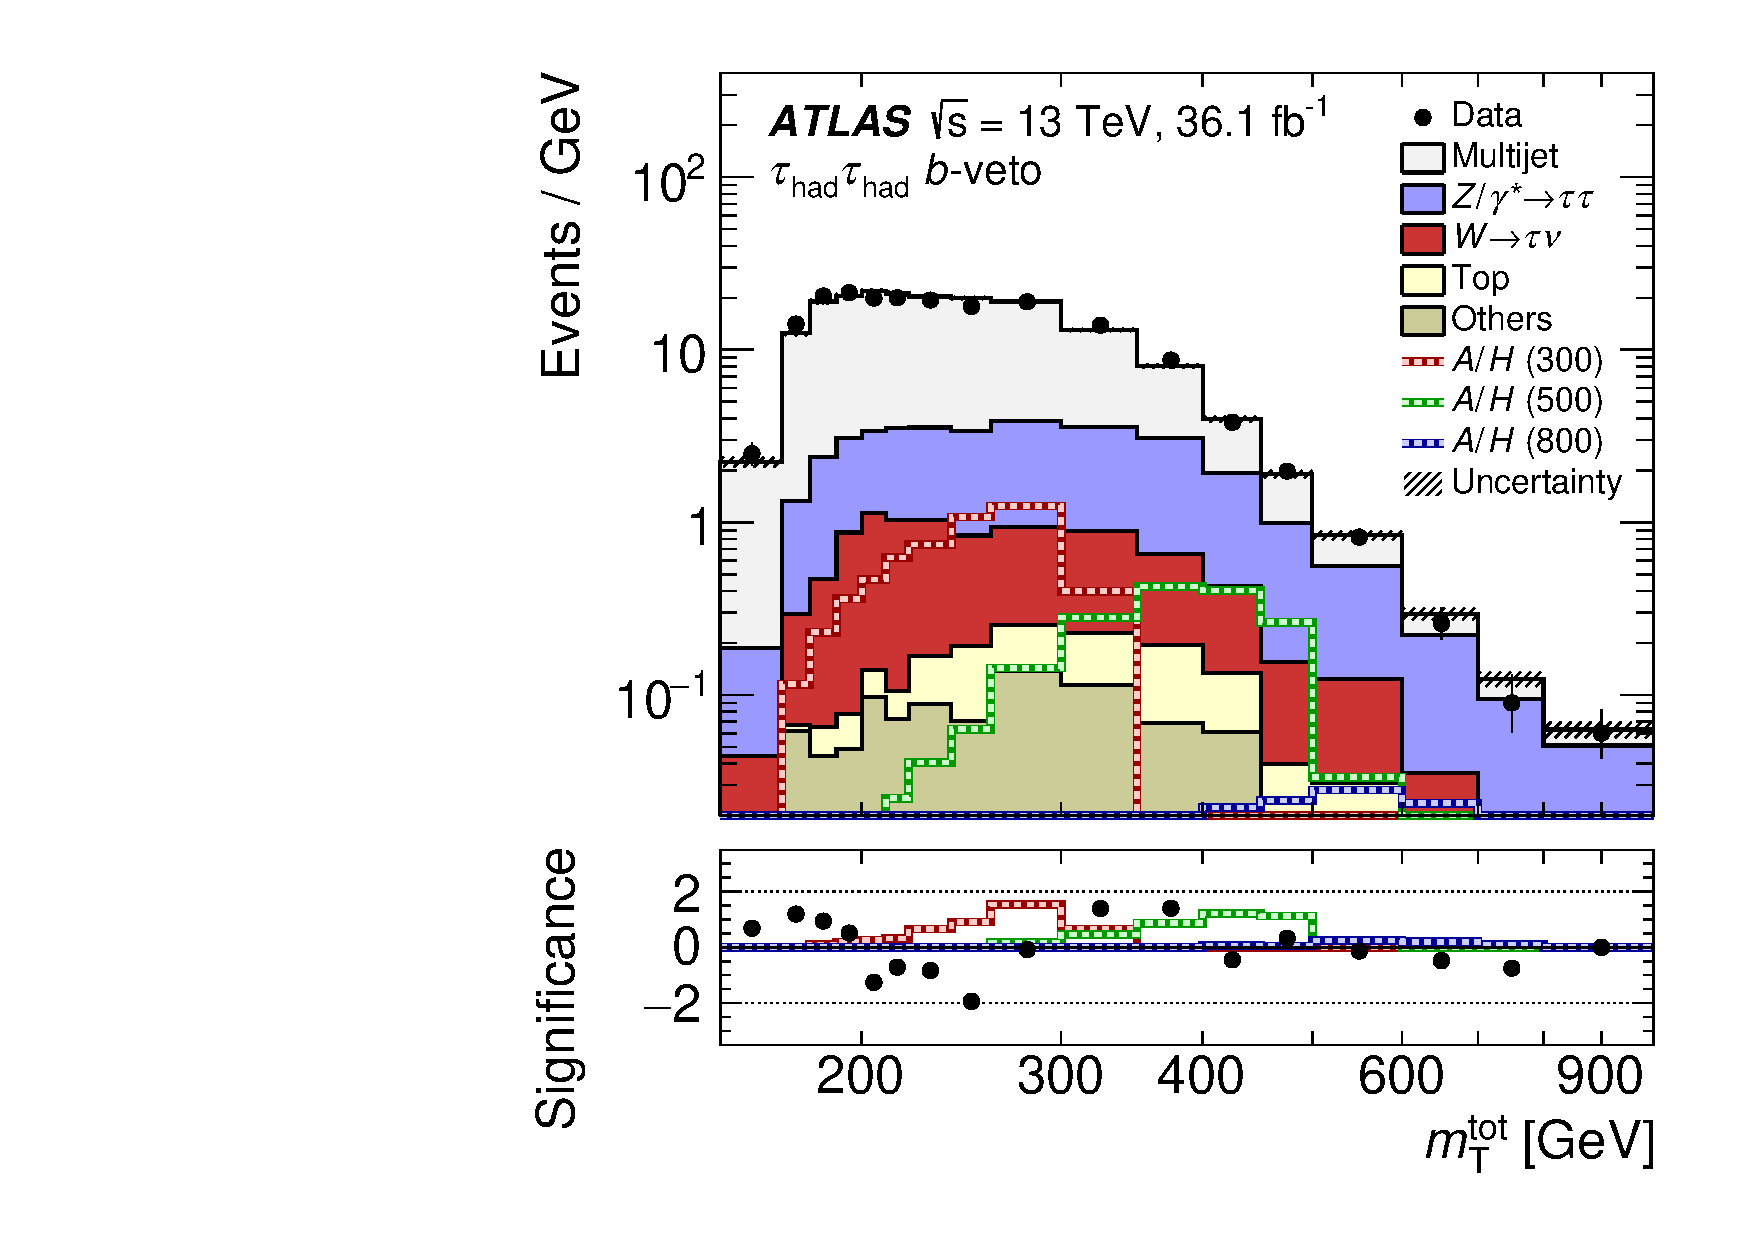
\includegraphics[width=0.994\textwidth]{./figures/theory/zprime_mttot.pdf}
    \subcaption{$A / H / Z^\prime \to \tau\tau$~\cite{zprime}}
  \end{subfigure}
  \caption{Comparison of the background rejection of the RNN-based
    identification at a working point (WP) with increased signal efficiency with
    the nominal tight working point of the BDT.}
  \label{fig:loosened_wp}
\end{figure}



Fakes contain fake taus and fake leptons. Where fake taus originate from jets
originating from quarks- or gluons in multijet, $Z+\text{jets}$, $W+\text{jets}$

\begin{itemize}
  \item $Z \rightarrow \tau \tau$ (background for H$\tau \tau$ and
    useful for performance measurements using tag-and-probe -- semileptonic
    decays)

  \item $Z \to \tau\tau$ or $H \to \tau\tau$ polarisation measurements

  \item $H \rightarrow \tau \tau$ (one of two channels to measure
    the fermionic coupling -- $b \bar{b}$ plagued by multijet background,
    Higgs CP)

  \item $t\bar{t}H$ with $H \to \tau \tau$: $H \to b \bar{b}$ large backgrounds.
    Associative production with top quarks to measure Yukawa coupling between
    top and higgs.

  \item MSSM Higgs (potentially high branching fraction to $\tau$-leptons)

  \item $Z^\prime$ could preferentially decay into third-generation
    fermions (lepton universality not required).

  \item $W^\prime$ models with preferential coupling to third-gen.

  \item SUSY with $\tau$ \textrightarrow long decay chains (Desch)

  \item Beyond the Standard Model (SUSY -- preferred coupling to down-type
    fermions for large $\tan\beta$ \textrightarrow $\tau$-leptons)
\end{itemize}

%%% Local Variables:
%%% mode: latex
%%% TeX-master: "mythesis"
%%% End:

% ~ 6 pages
\chapter{The ATLAS Experiment at the Large Hadron Collider}
\label{chap:atlas}

The ATLAS experiment is located at the LHC at CERN, a symmetric proton--proton
and heavy ion collider, supplying collision events to four major experiments. In
proton--proton operation, bunches of protons are crossed at the interaction
points located inside of the experiments with a peak bunch crossing rate
of~\SI{40}{\mega\hertz}~\cite{lhc}. With a proton beam energy of \SI{6.5}{\TeV}
during Run~2 of the LHC, the proton--collisions take place at a center-of-mass
energy of \SI{13}{\TeV}. During the 2016 data taking period, a peak
instantaneous luminosity of~\SI{1.4e34}{\per\square\centi\metre\per\second} was
reached~\cite{lhc_2016_report}, which was further increased during the 2017 data
taking period.

\section{Overview of the ATLAS Detector}
\label{sec:atlas}

The ATLAS detector, described in Ref.\ \cite{atlas_detector}, is a multipurpose
particle detector experiment. An overview of the detector is given in
Figure~\ref{fig:atlas_detector}. Its cylindrical geometry provides almost
$4\pi$~coverage and forward-backward symmetry with respect to the nominal
interaction point. Specialised detector subsystems are arranged in concentric
layers around the beam axis, enabling the reconstruction of photons, electrons,
muons, taus and jets. Moreover, the detector coverage allows to reconstruct
missing transverse energy from weakly and non-interacting particles.

\begin{figure}[htb]
  \centering
  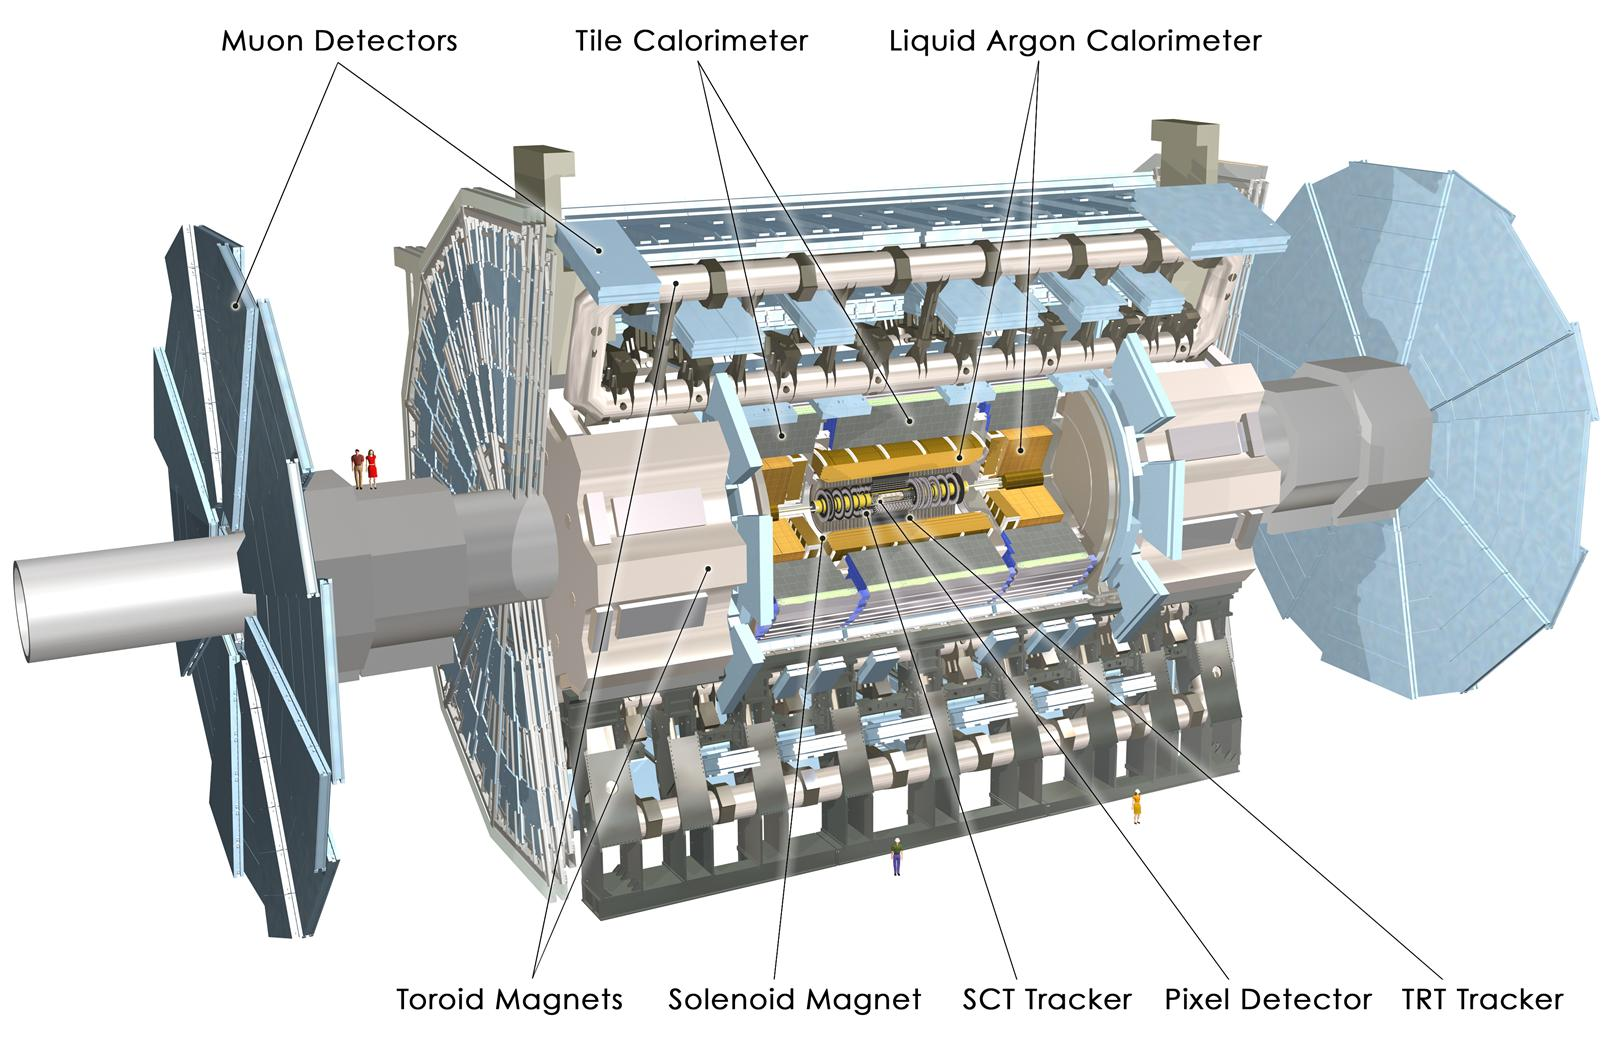
\includegraphics[width=0.8\textwidth]{./figures/atlas/overview.jpg}
  \caption[Overview of the ATLAS detector]{Overview of the ATLAS
    detector~\cite{atlas_detector}. Shown is the inner detector consisting of
    pixel, microstrip (SCT), transition radiation tracker (TRT) and solenoid;
    the calorimeter system consisting of LAr and Tile sampling calorimeters and
    the muon spectrometer consisting of tracking chambers and air-core toroids.}
  \label{fig:atlas_detector}
\end{figure}

In the ATLAS experiment a right-handed coordinate system is used to describe
positions in the detector. The origin of the coordinate system is located at the
nominal interaction point, with the $z$-axis pointing along the beam axis, the
$x$-axis towards the centre of the LHC ring and the $y$-axis upwards. The $x$-
and $y$-axes span the transverse plane. Spherical
coordinates~$(r, \varphi, \theta)$ are commonly used, with the azimuthal
angle~$\varphi$ being measured in the transverse plane and the polar
angle~$\theta$ with respect to the beam axis.

Due to the unknown longitudinal momentum of colliding partons in the
proton--proton collisions, the momentum of final state particles only balances
in the transverse plane. Therefore, transverse quantities for momentum and
energy are defined as
\begin{align*}
  p_\text{T} &= |\mathbf{p}| \sin\theta & E_\text{T} &= E \sin\theta \eqdot
\end{align*}
In addition, the unknown boost along the $z$-axis motivates the definition of
the pseudorapidity
\begin{align*}
  \eta &= -\ln\left[ \tan\left( \frac{\theta}{2} \right) \right] \eqcomma
\end{align*}
such that differences in~$\eta$ are Lorentz-invariant in the massless limit, and
the angular distance
\begin{align*}
  \Delta R &= \sqrt{\left(\Delta\eta\right)^2 + \left(\Delta\varphi\right)^2} \eqcomma
\end{align*}
where $\Delta \eta$ and $\Delta \varphi$ are the differences in pseudorapidity
and azimuthal angle, respectively.

In the following a brief description of the detector subsystems is given. In
increasing radial distance from the beam axis, the systems are:
\begin{description}
\item[Inner Detector] The inner detector (ID) consists of several layers of
  pixel detectors, silicon microstrip detectors and straw chambers. The ID is
  embedded in a \SI{2}{\tesla} axial magnetic field, bending the trajectories of
  charged particles in the transverse plane, thus allowing transverse momentum
  measurements. Hits of charged tracks in the active layers of the ID are
  reconstructed as so called space points, which are used to perform tracking
  and vertexing. The straw tubes of the Transition Radiation Tracker (TRT) offer
  tracking at large radii as well as electron identification via high-threshold
  hits originating from transition radiation of electrons crossing the polymer
  material between the straws.

\item[Calorimeter System] The sampling calorimeters used in the ATLAS detector
  allow to measure the energies of photons, electrons and hadrons. The
  calorimeter system consists of an electromagnetic calorimeter with high
  granularity, designed to reconstruct energy depositions of photons and
  electrons, and the coarser hadronic calorimeter to reconstruct jets of
  hadrons.

\item[Muon Spectrometer] Muons passing the calorimeter are measured in
  high-precision tracking chambers in the magnetic field of an air-core toroid.
  The spectrometer allows to identify muons and measure their momentum from the
  curvature of reconstructed tracks in the muon system.

\item[Trigger and Data Acquisition Systems] The peak event rate of
  \SI{40}{\mega\hertz} in the ATLAS detector, mostly consisting of events not of
  immediate interest for physics research, needs to be reduced in a trigger
  system to match the limited throughput of the data acquisition systems, while
  still being sensitive to rare physics processes. The trigger of the ATLAS
  detector is divided into three levels: L1, L2 and the event filter. They
  successively reduce the rate, while having access to detector information of
  increasing granularity. After the final trigger level, the event filter, the
  rate is sufficiently small, such that events can be moved to permanent storage
  for later analysis.
\end{description}
For the reconstruction of hadronic tau decays, the tracking and calorimeter
systems are of large importance. In the following they are described in more
detail.

\section{The Inner Detector}
\label{sec:atlas_tracking}

The inner detector of the ATLAS experiment provides track reconstruction in the
high particle density environment of proton--proton collisions at the LHC. The
tracking system meets the transverse momentum and vertex resolution requirements
needed to perform physics analyses. An overview of the inner detector is shown
in Figure~\ref{fig:atlas_indet}.

\begin{figure}[htb]
  \centering
  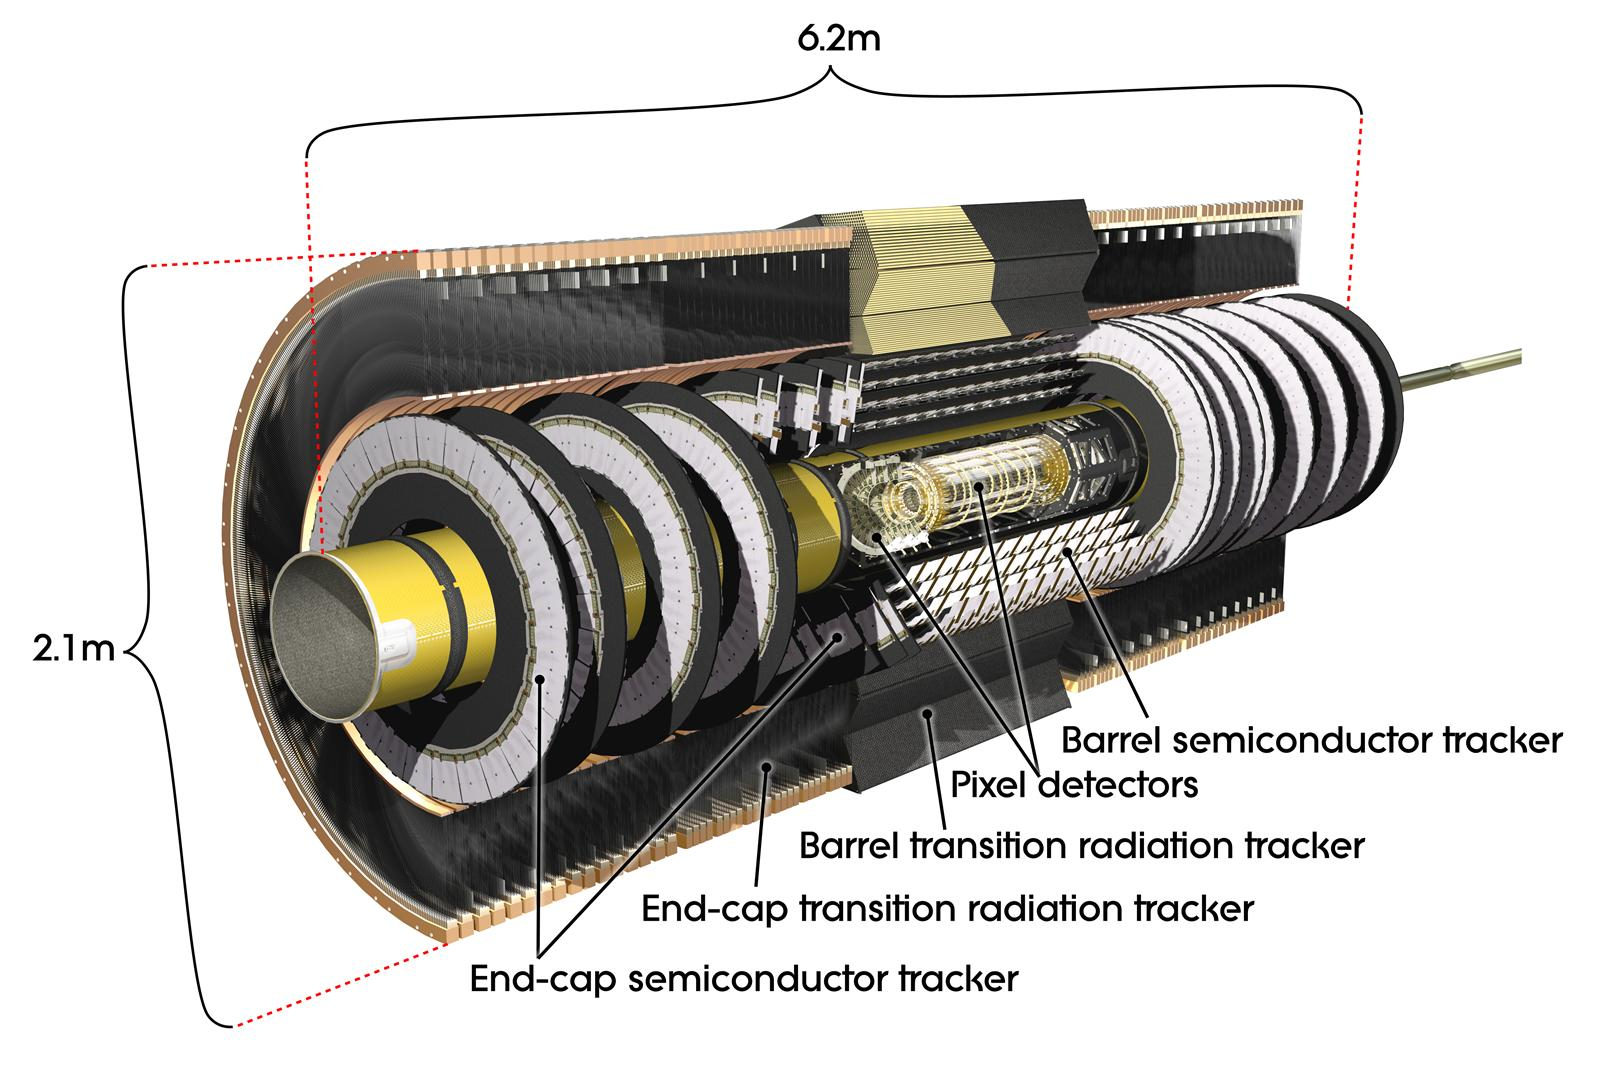
\includegraphics[width=0.75\textwidth]{./figures/atlas/inner_detector.jpg}
  \caption[Overview of the ATLAS inner detector]{Overview of the ATLAS inner
    detector~\cite{indet_fig}. Shown are pixel and microstrip detector as well
    as the Transition Radiation Tracker. The innermost pixel layer, the
    Insertable B-Layer, is not depicted.}
  \label{fig:atlas_indet}
\end{figure}

The inner detector consists of three distinct and complementary parts employing
different detector technologies. From the interaction point outwards, it
consists of: pixel detectors, silicon microstrip detectors and a transition
radiation detector using drift tubes.

The pixel detectors consist of the Insertable B-Layer (IBL), installed during
Long~Shutdown~1 at a reduced distance from the interaction point
of~$r = \SI{33.25}{\milli\metre}$~\cite{ibl_tdr}, and three additional layers
spanning radial distances from \SI{50.5}{\milli\metre} to
\SI{122.5}{\milli\metre}~\cite{atlas_detector} in the barrel of the ATLAS
detector. Additionally, three disks of pixel detectors cover the forward and
backward regions in two endcaps. The sensors of the IBL provide an intrinsic
resolution of approximately \SI{10}{\micro\metre} in the azimuthal ($r\varphi$)
direction and \SI{65}{\micro\metre} in $z$-direction~\cite{ibl_measurement}. The
other pixel layers have resolutions of \SI{10}{\micro\metre} in $r\varphi$ and
\SI{115}{\micro\metre} in $z$-direction~\cite{atlas_detector}. The high
resolution of the pixel detectors and their proximity to the interaction point
are crucial for track impact parameter measurements (cf.\
Figure~\ref{fig:impact_params}) and for primary as well as secondary vertex
reconstruction.

\begin{figure}[htb]
  \begin{subfigure}[t]{0.48\textwidth}
    \centering
    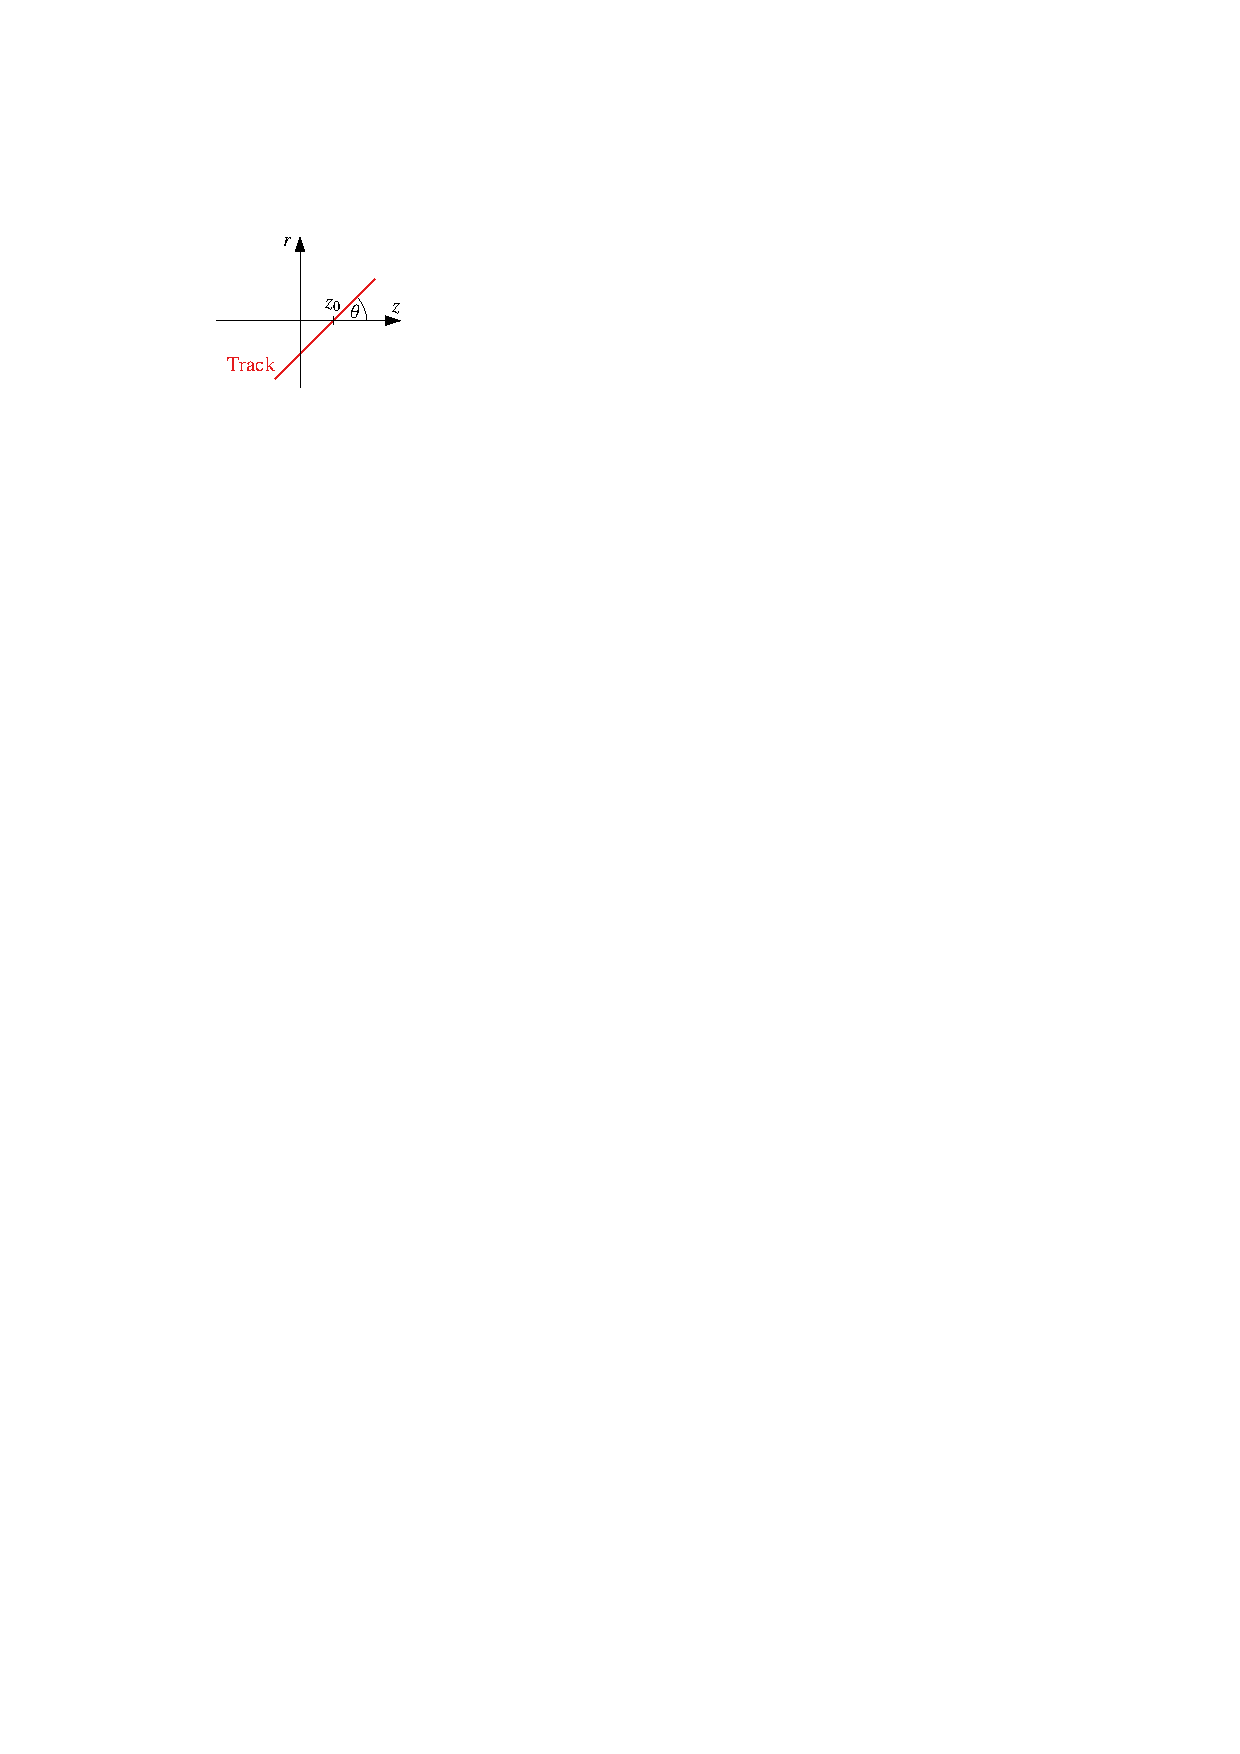
\includegraphics{./figures/atlas/impact_params_z0.pdf}
    \subcaption{Definition of the longitudinal impact parameter, $z_0$.}
    \label{fig:longitudinal_impact_param}
  \end{subfigure}\hfill
  \begin{subfigure}[t]{0.48\textwidth}
    \centering 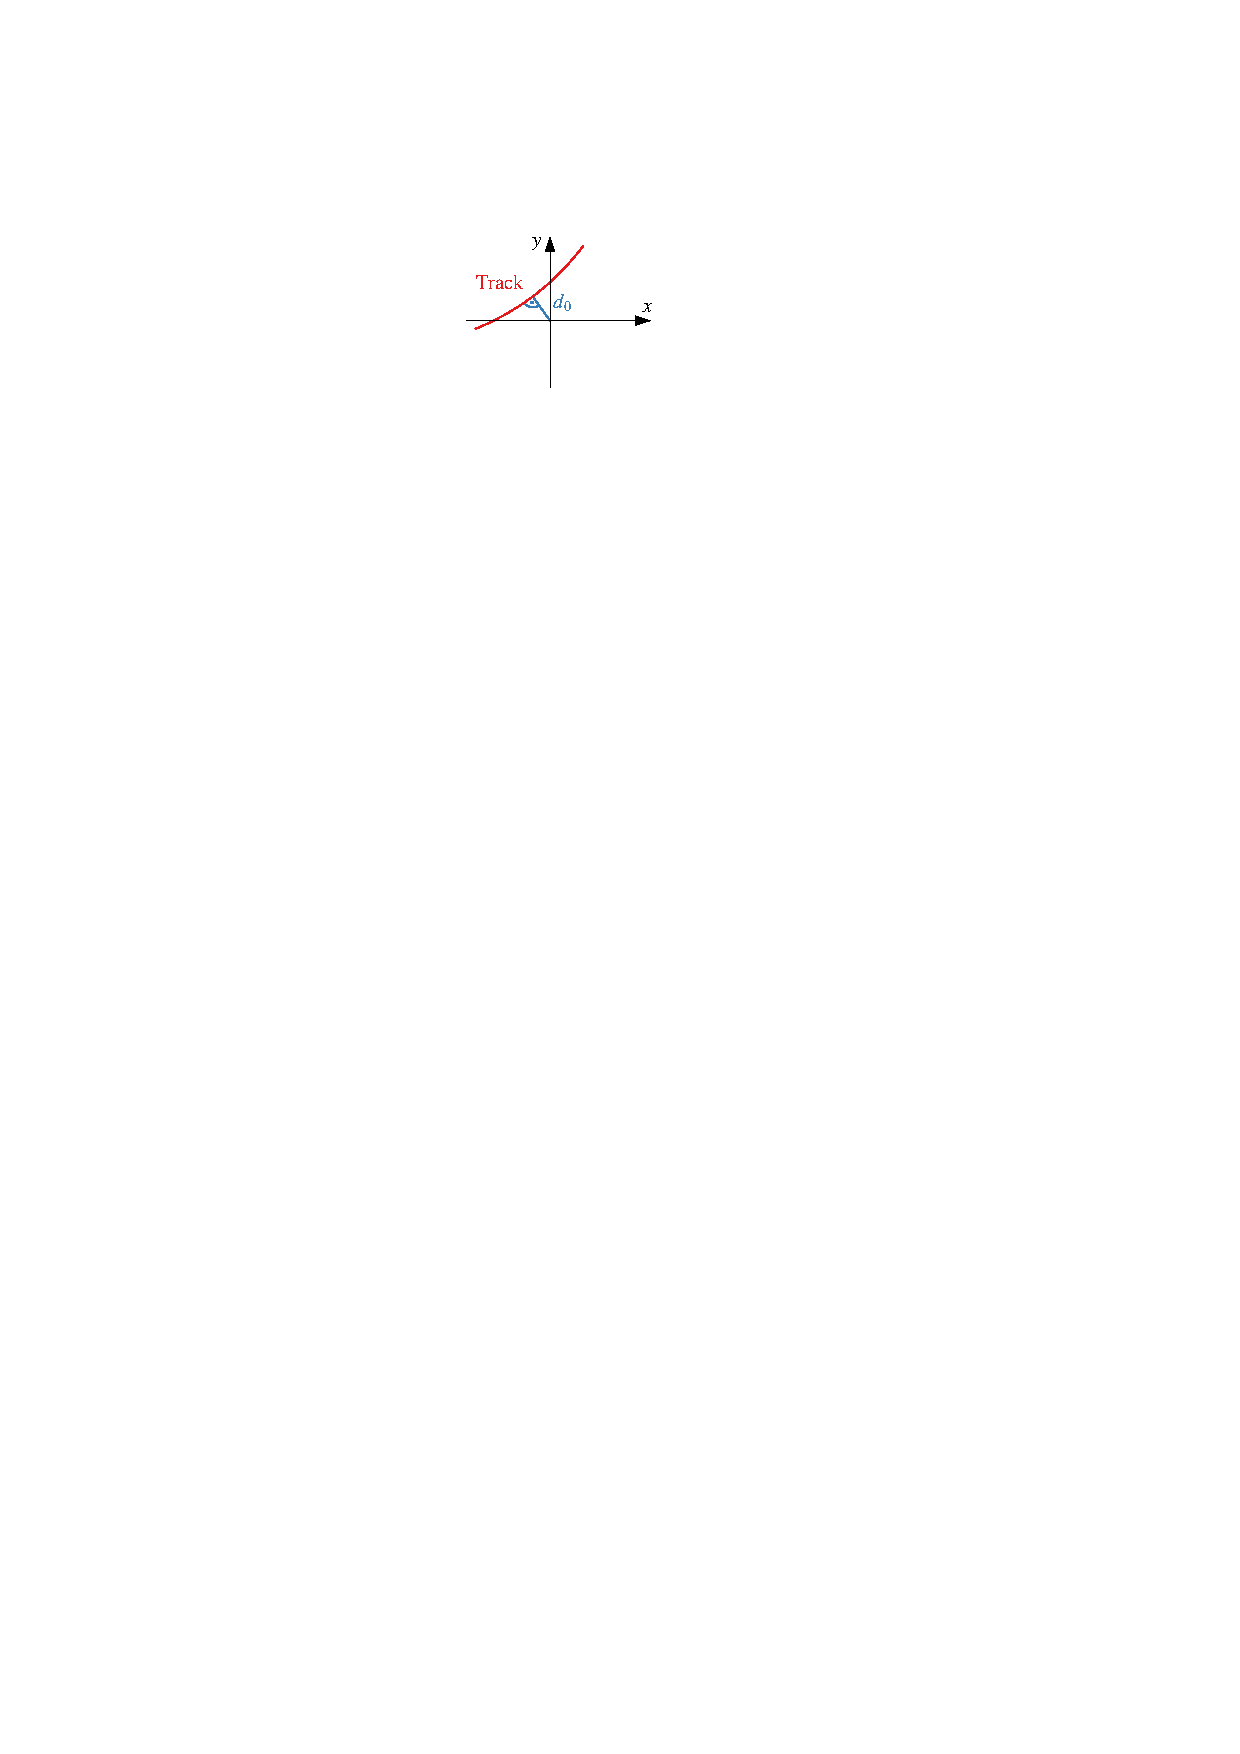
\includegraphics{./figures/atlas/impact_params_d0.pdf}
    \subcaption{Definition of the transverse impact parameter, $d_0$. The sign
      of $d_0$ depends on the angular momentum of the track w.r.t.\ the origin.}
    \label{fig:transverse_impact_param}
  \end{subfigure}
  \caption[Definition of track impact parameters]{Definition of track impact
    parameters at the perigee with respect to the origin.}
  \label{fig:impact_params}
\end{figure}

The Semiconductor Tracker (SCT) is a silicon microstrip detector with four
barrel layers covering the intermediate radial range from
$r = \SI{299}{\milli\metre}$ to \SI{514}{mm}~\cite{atlas_detector}. In the
endcaps, the SCT consists of nine disks perpendicular to the beam axis. The
intrinsic resolution of the SCT sensors is \SI{17}{\micro\metre} in $r\varphi$
and \SI{580}{\micro\metre} in axial (radial) direction for the barrel
(disks)~\cite{atlas_detector}. The semiconductor tracking detectors provide a
pseudorapidity coverage of approximately~$|\eta| < 2.5$.

Track measurement at large radial ranges of $r = \SI{554}{\milli\metre}$ to
\SI{1082}{\milli\metre} are provided by the TRT consisting of drift tubes with a
diameter of \SI{4}{\milli\metre} aligned with the beam
axis~\cite{atlas_detector}. As a result, they only provide azimuthal
measurements with an intrinsic resolution of
\SI{130}{\micro\metre}~\cite{atlas_detector}. With a large number of 73 (160)
straw planes in the barrel (endcap) it provides tracking and electron
identification over a pseudorapidity range
of~$|\eta| < 2.0$~\cite{atlas_detector}.

Charged-particle tracks are reconstructed from space points using sophisticated
pattern-recognition and tracking algorithms. After reconstruction, several
representations can be used to define tracks. In the ATLAS detector, tracks are
often represented at the perigee with respect to a reference point, which is
commonly the primary vertex or the beamspot. In this representation tracks are
unambiguously defined by the transverse and longitudinal impact parameters,
$d_0$ and $z_0$ (cf.\ Figure~\ref{fig:impact_params}), the azimuthal and polar
angles of the track momentum vector at the perigee, $\varphi$ and $\theta$, as
well as the ratio of charge and momentum of the track, $q / p$.

% See \url{https://twiki.cern.ch/twiki/bin/view/AtlasProtected/InDetTrackingDC14#Impact_parameters_z0_d0_definiti}

\section{The Calorimeter System}
\label{sec:atlas_calo}

The ATLAS calorimeter system, shown in Figure~\ref{fig:atlas_calo}, employs
sampling calorimeters to measure the energy depositions of charged and neutral
particles in the calorimeter material. With separate calorimeters for the
barrel, endcap and forward region, it
covers~\mbox{$|\eta| < 4.9$}~\cite{atlas_detector}. The calorimeter is divided
into two parts, the electromagnetic (EM) and the hadronic calorimeter, which are
further subdivided into longitudinal samplings of varying thickness and
granularity, thus allowing the measurement of longitudinal and transverse shower
shapes. The EM calorimeter has a thickness of more than 22 to 24 radiation
lengths\footnote{The radiation length~$X_0$ is the mean distance a high-energy
  electron passes through matter, until it loses all but~$e^{-1}$ of its initial
  energy due to bremsstrahlung.} depending on the detector
region~\cite{atlas_detector}, which is sufficient to contain most
electromagnetic showers from electrons and photons. The combined thickness of EM
and hadronic calorimeter is approximately ten interaction lengths\footnote{The
  interaction length~$\lambda$ is the mean distance a high-energy hadron passes
  through matter, until it performs an inelastic collision with a
  nucleon.}~\cite{atlas_detector}, reducing punch-through of hadrons into the
muon spectrometer and allowing to reconstruct the missing transverse energy.

\begin{figure}[htb]
  \centering
  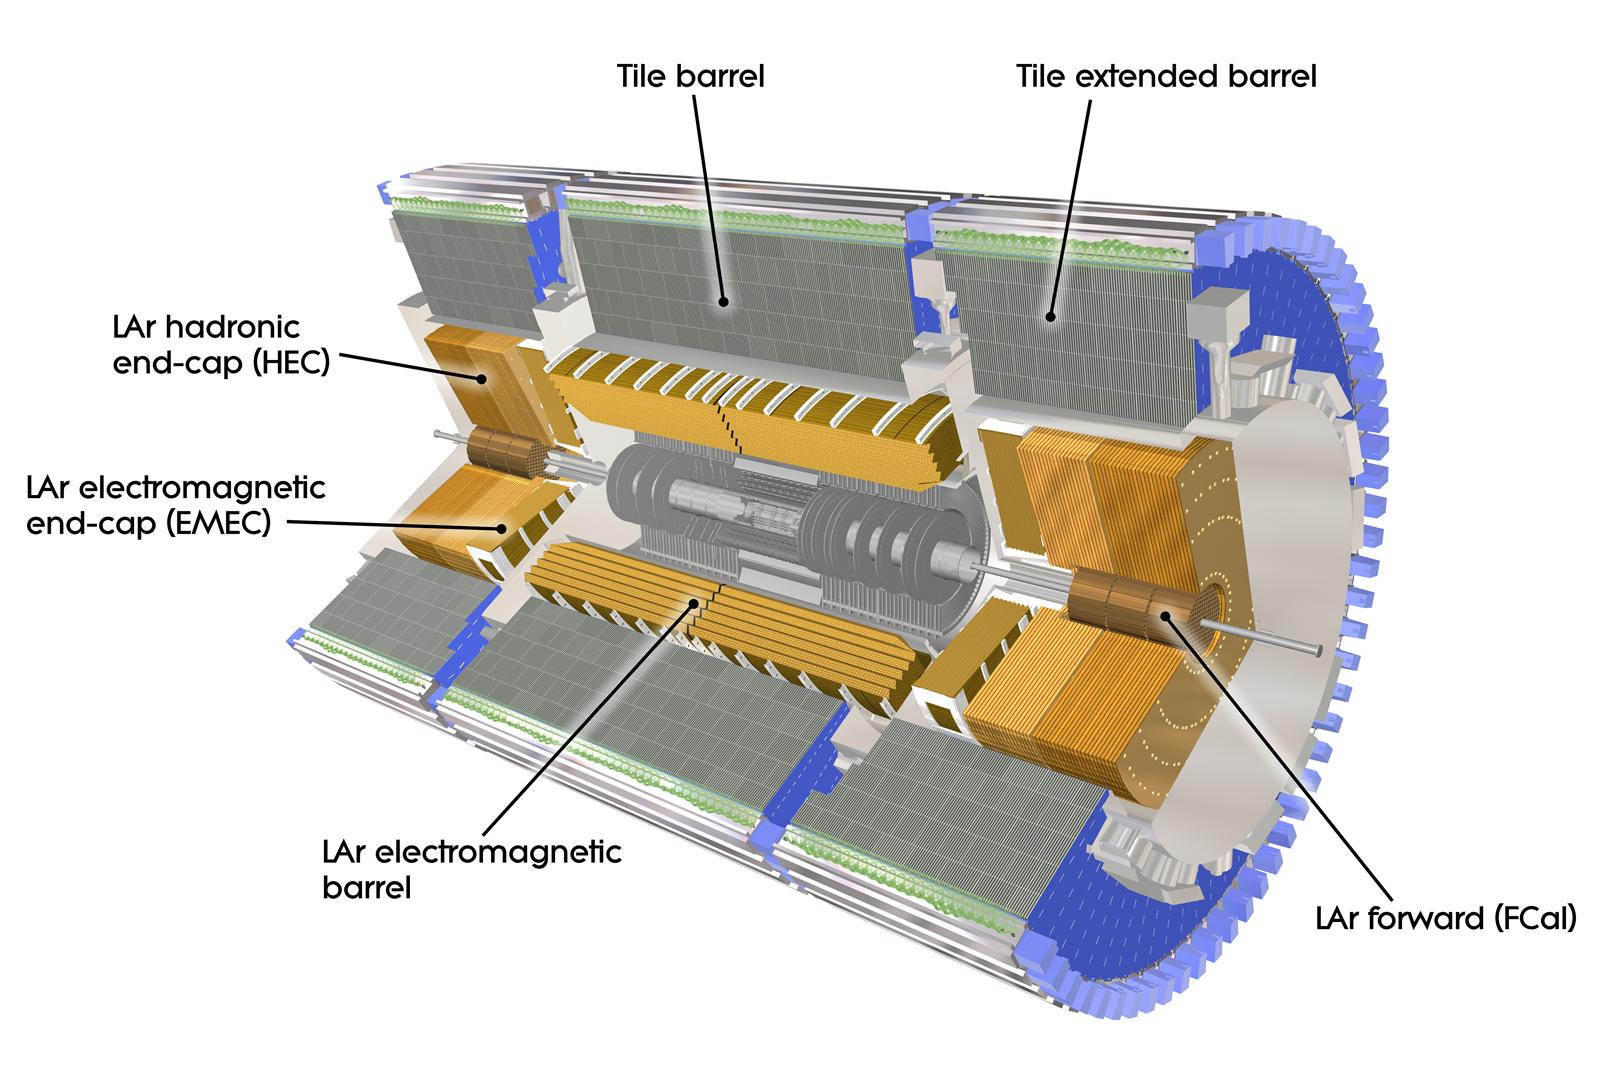
\includegraphics[width=0.8\textwidth]{./figures/atlas/calorimeter.jpg}
  \caption[Overview of the ATLAS calorimeter system]{Overview of the ATLAS
    calorimeter system~\cite{calo_fig}.}
  \label{fig:atlas_calo}
\end{figure}

The EM calorimeter uses liquid-argon (LAr) as the active material and lead
absorber plates. It is divided into a barrel (EMB) and two endcaps (EMEC),
covering the regions~$|\eta| < 1.475$ and $1.375 < |\eta| < 3.2$,
respectively~\cite{atlas_detector}. With the exception of the transition region
between barrel and endcap, $1.35 < |\eta| < 1.5$, and the forward region,
$|\eta| > 2.5$, the LAr EM calorimeter consists of three longitudinal
samplings~\cite{atlas_detector}. The following description focuses on the
region~$|\eta| < 2.5$ used for high-precision measurements, while also excluding
the transition region. The innermost sampling of the EM calorimeter (EM1), also
called the strip layer, is finely segmented in $\eta$-direction with a cell
segmentation of~$\Delta\eta \times \Delta\varphi = 0.025/8 \times 0.1$ with
decreasing $\eta$-granularity in the EMEC~\cite{atlas_detector}. The second and
third layer (EM2 and EM3) have a granularity of~$0.025 \times 0.025$
and~$0.050 \times 0.025$ in~$\Delta\eta \times \Delta\varphi$,
respectively~\cite{atlas_detector}. The thickness of the three layers
at~$\eta = 0$ is approximately~$4.5 X_0$, $17 X_0$ and $1.5 X_0$ for EM1, EM2
and EM3, respectively~\cite{atlas_detector}. As a result, high-energy electrons
and photons deposit a most of their energy in EM2. An active LAr layer precedes
the EM calorimeter in the region $|\eta| < 1.8$ to correct for energy losses
upstream of the calorimeter system~\cite{atlas_detector}.

For hadron calorimetry the ATLAS experiment uses two different calorimeter types
in the barrel and endcap regions. In the barrel, a sampling calorimeter based on
steel absorbers and plastic scintillating tiles, the so called tile calorimeter,
is used. It is separated into a barrel part, $|\eta| < 1.0$, and two extended
barrels, $0.8 < |\eta| < 1.7$ (cf.\ Figure~\ref{fig:atlas_calo}). Similar to the
LAr EM calorimeter, the tile calorimeter is segmented into three longitudinal
samplings. The lateral segmentation of these layers is~$0.1 \times 0.1$ in the
first two layers and~$0.2 \times 0.1$ in the last layer~\cite{atlas_detector}.
The hadronic endcap calorimeter (HEC), located behind the EMEC, uses LAr as the
active material and copper absorbers. The HEC provides a pseudorapidity coverage
of $1.5 < |\eta| < 3.2$, partially overlapping the tile extended barrel, with
four longitudinal samplings. The granularity in the region~$|\eta| < 2.5$ is
$0.1 \times 0.1$~\cite{atlas_detector}.

\subsection{Topological Cell Clustering}

In the ATLAS experiment a topological cell clustering algorithm is used to
reconstruct three-dimensional energy depositions in the calorimeter system,
while suppressing noise from calorimeter cells not topologically connected to
cells with significant signal strength. The TopoCluster
algorithm~\cite{atlas_topoclustering} used in the ATLAS experiment operates on
cells of the calorimeter calibrated at the electromagnetic energy scale,
therefore not accounting for the different calorimeter response to hadronic
showers. The cluster formation is seeded by the cell of largest signal
significance~\cite{atlas_topoclustering}
\begin{align*}
  \varsigma_\text{cell}^\text{EM} = \frac{E_\text{cell}^\text{EM}}{\sigma_\text{noise,cell}^\text{EM}} \eqcomma
\end{align*}
where~$E_\text{cell}^\text{EM}$ is the cell signal
and~$\sigma_\text{noise,cell}^\text{EM}$ the estimated noise of the cell, if it
passes a seed threshold of~$|\varsigma_\text{cell}^\text{EM}| > 4$. The cluster
is expanded by including neighbouring cells in the same and adjacent layers of
the calorimeter that pass a cell significance threshold
of~$|\varsigma_\text{cell}^\text{EM}| > 2$. If a neighbouring cell is a seed
cell or a cell associated to another cluster passing
the~$|\varsigma_\text{cell}^\text{EM}| > 2$ threshold, both clusters are merged.
The process is repeated until the last cell passing the threshold has been
included. Afterwards, all adjacent cells are included into the cluster
independent of their signal significance to account for signals close to the
noise level~\cite{atlas_topoclustering}. If a cluster has multiple local maxima,
it is split in all three spatial dimensions to more accurately reflect the
substructure of the cluster. After cluster splitting, cells at the interface of
two clusters can be shared between them according to an assigned weight to each
cluster.

The geometrical shape and distribution of cell signals in a TopoCluster is
characterised by so called cluster moments. The $n$-th moment of a cell
variable~$v_\text{cell}$ is given by \cite{atlas_topoclustering}
\begin{align*}
  \langle v_\text{cell}^n \rangle = \frac{\sum_{i \mid E_{\text{cell,}i}^\text{EM} > 0} w_{\text{cell,}i} \, E_{\text{cell,}i}^\text{EM} \, v_{\text{cell,}i}^n}{\sum_{i \mid E_{\text{cell,}i}^\text{EM} > 0} w_{\text{cell,}i} \, E_{\text{cell,}i}^\text{EM}} \eqcomma
\end{align*}
where $w_{\text{cell,}i}$ is the weight of the cell in the cluster and
out-of-time signals, $E_\text{cell}^\text{EM} < 0$, are not considered. An
example is the first moment of the Cartesian coordinates of a cell centre,
defining the barycentre of a cluster.

\subsection{Local Hadronic Calibration}
\label{sec:local_hadronic_calib}

The calorimeters of the ATLAS detector are non-compensating, meaning their
response differs for electromagnetic and hadronic showers originating from
particles of the same energy. The local hadronic calibration (LC), described in
Ref.~\cite{atlas_topoclustering}, provides a calibration for clusters
reconstructed with the TopoCluster algorithm without prior assumption of the
particle that created it. The LC scale accounts for the non-compensating nature
of the calorimeters, out-of-cluster energy and dead
material~\cite{atlas_topoclustering}.

The calibration procedure begins with clusters at the electromagnetic energy
scale. Cluster moments determined by the TopoCluster algorithm allow to
discriminate between clusters created by electromagnetic and hadronic energy
deposits. Depending on a likelihood~$\mathcal{P}_\text{clus}^\text{EM}$,
characterising the probability of a cluster to originate from an electromagnetic
shower, a hadronic calibration is applied to the cells of a cluster. This
accounts for the non-compensation of the calorimeter on a cluster-by-cluster
basis. Additional calibration factors are applied to account for signal loss due
to clustering. Due to the inherent noise suppression of the TopoCluster
algorithm, cells with small signal contributions can be lost during clustering.


factor for hadronic showers is applied to the cluster to correct the
non-compensation.

Additional calibrations factors are applied to account for signal loss due to
cells being omitted from the cluster due to the noise suppression of the
TopoCluster algorithm and dead material.

%%% Local Variables:
%%% mode: latex
%%% TeX-master: "mythesis"
%%% End:

% ~ 3-4 pages
\chapter{Reconstruction and Energy Calibration of Hadronic Tau Lepton Decays}
\label{sec:reconstruction}

% TauBuilder config:
% https://gitlab.cern.ch/atlas/athena/blob/master/Reconstruction/tauRec/python/TauRecBuilder.py
%
% AlgHolders:
% https://gitlab.cern.ch/atlas/athena/blob/master/Reconstruction/tauRec/python/TauAlgorithmsHolder.py
%
This chapter describes the offline reconstruction of hadronic tau decays used in
the ATLAS experiment. It summarises the reconstruction as given in Refs.\
\cite{atlas:taurec:run1, atlas:taurec:run2}, while also including recent changes
to the reconstruction algorithms. The recent changes are compiled from
documentation available in the tau reconstruction packages of the ATLAS software
framework~\textsc{Athena}~\cite{athena}. The introduction of a charged-particle
track selection and classification using multivariate methods~\cite{duschinger}
has the largest impact on the work presented in this thesis.

% JetSeedBuilder:
% https://gitlab.cern.ch/atlas/athena/blob/master/Reconstruction/tauRecTools/src/JetSeedBuilder.cxx
Candidates for \tauhadvis are seeded by jets formed by the anti-$k_t$ jet
algorithm~\cite{antikt} using a distance parameter of $R = 0.4$ on
three-dimensional clusters of calorimeter cells called \emph{TopoClusters}. The
clusters are calibrated using a local hadronic calibration (LC) to account for
the non-compensating nature of the calorimeter, dead material and out-of-cluster
energy~\cite{local_hadronic_calib}. To seed a \tauhadvis candidate the jet has
to satisfy~$p_\text{T} > \SI{10}{\GeV}$ and is required to fall in the
acceptance range of the tracking system~$|\eta| < \num{2.5}$.
% At this step tau $p_\mathrm{T}, \eta, \varphi, m$ ($m$: invariant mass) are
% set to the ones of the jet seed -- what does this mean? Read up on jet algs

\section{Vertex Association}
\label{sec:reco_vertex_assoc}
% TauVertexFinder:
% https://gitlab.cern.ch/atlas/athena/blob/master/Reconstruction/tauRecTools/src/TauVertexFinder.cxx
%
% Vertex association: Tracks matched unambiguously to jets via ghost-matching by
% adding all tracks into constituent list for the jet algorithm but setting
% their energy infinitesimally small (such that the result of the jet algorithm
% is not affected due to IR-safety) and rerunning the algorithm.
% \url{https://twiki.cern.ch/twiki/bin/view/AtlasProtected/JetGhostMatching}
%
% Tracking CP recommendations
% \url{https://twiki.cern.ch/twiki/bin/view/AtlasProtected/TrackingCPPreRecsSummer2017#Track_to_Vertex_Association}
In events with multiple primary vertices the tau production vertex has to be
identified. For this reconstructed charged-particle tracks that are matched to
the jet via ghost-matching~\cite{ghost_matching} are used.
% via ghost-matching\footnote{Tracks matched unambiguously to calorimeter jets
% by adding the tracks with infinitesimal energy to the constituent list
% and rerunning the jet algorithm.}
Tracks lying in a cone with radius~$\Delta R < 0.2$ with respect to the jet
axis, fulfilling~$p_\text{T} > \SI{1}{\GeV}$ and basic track quality
criteria\footnote{The specific requirements are: number of pixel
  hits~$N_\text{pixel} \geq 2$, number of silicon
  hits~$N_\text{Si} = N_\text{pixel} + N_\text{SCT} \geq 7$. Dead sensors on the
  trajectory are also counted.} are selected for vertex association.
% and lie in a cone with
% radius~$\Delta R < 0.2$ with respect to the jet axis are selected. Tracks that
% fulfil $p_\text{T} > \SI{1}{\GeV}$ and basic track quality criteria\footnote{The
%   specific requirements are: number of pixel hits~$N_\text{pixel} \geq 2$,
%   number of silicon hits~$N_\text{Si} = N_\text{pixel} + N_\text{SCT} \geq 7$.
%   Dead sensors on the trajectory are also counted.} are used for vertex
% association.
The primary vertex maximising the so called \emph{Jet Vertex
  Fraction}~(JVF)
\begin{align*}
  \text{JVF} = \frac{p_\text{T}\text{-sum of selected tracks assigned to the vertex}}{p_\text{T}\text{-sum of selected tracks}}
\end{align*}
% \begin{align*}
%   \mathrm{JVF} = \frac{\sum_\text{Vtx.\ \& TJVA} p_\mathrm{T}}
%                                            {\sum_\text{TJVA} p_\mathrm{T}}
% \end{align*}
is associated to the \tauhadvis candidate.
% \footnote{Impact parameter based association with the
%   primary vertex. $|d_0| < \SI{2.5}{mm}$ with respect to beamline and
%   $|(\Delta z_0) \sin\theta| < \SI{3}{mm}$. $\Delta z_0$ is the longitudinal
%   distance of vertex and track}

% TauAxisSetter:
% https://gitlab.cern.ch/atlas/athena/blob/master/Reconstruction/tauRecTools/src/TauAxisSetter.cxx
After the primary vertex is found, the preliminary four-momentum of the
\tauhadvis candidate is calculated.
% Assuming constituents have zero mass.
For this the barycentre of cluster energy at LC scale in the jet is determined.
The four-momentum of each jet constituent in the coordinate system of the
associated vertex, falling within a cone of~$\Delta R < 0.2$ with respect to the
barycentre, is summed. This defines the visible tau momentum at LC scale and the
tau axis. The \tauhadvis \pt at LC scale is used as a baseline for further
energy calibrations.

\section{Track Selection and Classification}
\label{sec:reco_track_sel_classif}
% TauTrackFinder:
% https://gitlab.cern.ch/atlas/athena/blob/master/Reconstruction/tauRecTools/src/TauTrackFinder.cxx
%
% TauTrackClassifier:
% https://gitlab.cern.ch/atlas/athena/blob/master/Reconstruction/tauRecTools/Root/TauTrackClassifier.cxx
Tracks reconstructed in the inner detector are associated with a \tauhadvis
candidate if they are in a cone of size~$\Delta R < 0.4$ with respect to the tau
axis.
% The tracks are classified into core, wide, and other tracks: If the tracks
% fail track selection (pt > 1GeV, IPd0Max = 1mm, IPz0Max = 1.5mm, nHitPix >= 2,
% nHitSi >= 7) they are classified as 'other'.
%
% If the tracks are within the 0.2 cone they are called 'core' tracks otherwise
% if they fall into the 0.2 - 0.4 annulus they are classified as 'wide'.
%
% Loose track selection for charged pions according to TrackingCP:
% pt > 400 MeV (This cut is already applied at track reco)
% |eta| < 2.5
% NSi >= 7
% N^sh_mod <= 1 (Number of shared models = N^sh_Pix + N^sh_SCT / 2)
% N^hole_Si <= 2
% N^hole_Pix <= 1
%
% Dirk's talk in TauCP:
% https://indico.cern.ch/event/615208/contributions/2481630/attachments/1415563/2167141/TauCP_TrackClassificationTaskforce_20170220.pdf
For each reconstructed track a multi-class classification is performed
categorising them into one of four track categories: \emph{charged},
\emph{conversion}, \emph{isolation} and \emph{fake}. The \emph{charged} category
captures tracks likely originating from charged pions of the tau decay.
\emph{Conversion} tracks are created by long-lived secondary particles from
converted photons or hadronic interactions. \emph{Isolation} tracks are from
primary particles not originating from the tau decay and \emph{fake} tracks from
combinations of unrelated space points in the inner detector.

The multi-class classification is performed by using three Boosted Decision
Trees~(BDT) organised into two stages. In the first stage a single BDT performs
binary classification of tracks into one of two preliminary categories:
charged/conversion and isolation/fake. The second stage uses two BDTs to
separate the preliminary categories into the four final track categories. The
BDTs employ information on track momentum, impact parameters, number of hits in
the ID, high-threshold hits in the TRT, etc. \todo{Schematic of BDT setup -- ben}

The track classification is used to reconstruct the charge of the \tauhadvis by
summing the charge of all \emph{charged} tracks. The number of \emph{charged}
tracks also defines whether a \tauhadvis candidate is from a 1- or 3-prong
decay. The classification algorithm is optimised to reconstruct \tauhadvis with
the correct number of \emph{charged} tracks, such that the reconstruction
efficiency, which is the fraction of hadronic tau decays that are reconstructed
as a 1- or 3-prong \tauhadvis candidate, is maximised. Analyses often require
\tauhadvis to have one or three \emph{charged} tracks leading to a significant
reduction in candidates from quark- or gluon-initiated jets, which typically
have a larger track multiplicity. Using the \emph{charged} classification a
derived track category is defined to calculate isolation variables. The
\emph{modified isolation} category consists of tracks not classified as
\emph{charged} and passing track selection criteria:\todo{Why not use isolation
  tracks?}
\begin{align*}
  &p_\text{T} > \SI{1}{\GeV} & &d_0^\text{PV} < \SI{1}{mm} & &|z_0^\text{PV} \sin\theta| < \SI{1.5}{mm} \\
  &N_\text{pixel} \geq 2 & &N_\text{Si} \geq 7 \eqcomma
\end{align*} \todo{define silicon hits}
where $d_0^\text{PV}$ ($z_0^\text{PV}$) is the transverse (longitudinal) impact
parameter with respect to the associated primary vertex and $N_\text{pixel}$
($N_\text{Si}$) the number of pixel (silicon) hits including dead sensors on the
trajectory. Tracks in the \emph{modified isolation} category are used to
calculate discriminants, e.g.\ the momentum fraction of isolation tracks, for
tau identification.

% \begin{figure}[htb]
%   \centering
%   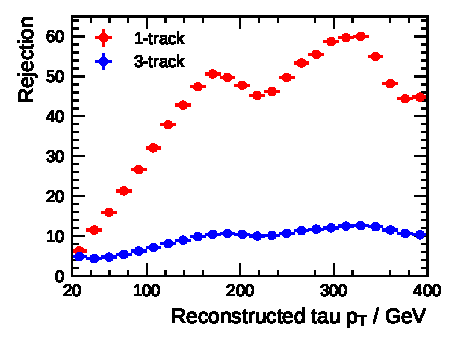
\includegraphics{./figures/bdt_perf/mva_tracking_rejection.pdf}
%   \caption{Rejection due to MVA tracking. Rejection of tau candidates from
%     dijets after baseline tau selection.}
%   \label{fig:mva_tracking_rejection}
%   \todo[inline]{Ticks are fucked. Increasing rejection with pt \textrightarrow
%     increasing multiplicity of jets with higher pt. Might be a problem with
%     weighting scheme?}
% \end{figure}

% Tau Tracks: tracks from the direct tau decay (pions)
%
% Conversion Tracks: tracks from conversions, hadronic interactions, 'long'
% living particles MVA Tracking input (barcode > 200k -- secondary particles)
%
% Isolation Tracks: mainly tracks from the underlying event (barcode < 10k but
% not tau tracks)
%
% Fake Tracks: not truth matched (10k < barcode < 200k) (includes pilup?)
%
% barcode < 200k -- primary particles
%
% variables: jetseed pt, track eta, z0SinThetaTJVA, rConvII, dRJetSeedAxis, d0,
% qOverP, nInnermostPixelHits, nPixelSharedHits, nSCTSharedHits, eProbabilityHT,
% nPixHits, nSiHits
% Impact params: reject conversion (d0), isolation and fake tracks (z0)
% Pixel, Si-Hits: rejection against conversions (missing hits)
% shared hits: intent is to recover merged tracks
% eProbabilityHT: Conversion tracks
% qOverP, dR: IT, FT

\section{Energy Calibration}
\label{sec:reco_energy_calib}
% TauCalibrateLC:
% https://gitlab.cern.ch/atlas/athena/blob/master/Reconstruction/tauRecTools/Root/TauCalibrateLC.cxx
%
% 5 eta bins: [0.0, 0.3, 0.8, 1.3, 1.6, 2.4]
% pile-up slopes for 1P and 3P for each eta bin
% mean pile-up for 1P and 3P
% A calibration function for 1P and 3P for each bin
%
% Offset calculated as
% offset = slope * (reco. num of PU vertices - average number of PU vertices)
% energyLC = ptDetectorAxis()
% if energyLC - offset <= 0: set offset to 0
% energyPUCorr = energyLC - offset
% calibConst = func(nProng, eta; energyPUCorr)
% if calibConst <= 0: calibConst = 1.0
% energyFinal = energyPUCorr / calibConst
%
The visible momentum measurement of the tau decay at LC scale is not optimised
to accurately reflect the true visible momentum. Additional corrections for
energy contributions due to pile-up, energy depositions outside of the
$\Delta R < 0.2$ cone and detector responses in different regions need to be
taken into account. Therefore, an energy calibration is applied to the
reconstructed object to reduce bias and improve the resolution of the energy
measurement. The calibration is applied to the \tauhadvis \pt at LC scale which
is related to the visible energy~$E_\text{vis}$ given the mass and
pseudorapidity of the \tauhadvis candidate.

The visible transverse momentum at LC scale~$p_\text{T}^\text{LC}$ increases
linearly with the number of reconstructed primary vertices~$N_\text{PV}$
\todo{Plot?}. Therefore, the pile-up contribution to the transverse momentum is
estimated by~\cite{atlas:taurec:run2, calo_tes}
\begin{align*}
  p_\text{T}^\text{pileup}(N_\text{PV}, |\eta|, n_\text{p}) &= A(|\eta|, n_\text{p}) \times N_\text{PV} \eqcomma
\end{align*}
where $A$ is the average pile-up contribution per reconstructed vertex,
parametrised in bins of~$|\eta|$ and separately for 1- and multi-prong
decays~$n_\text{p}$. The pile-up correction is of the order of~\SI{0.1}{\GeV}
per vertex.
% A is roughly of the order of 0.1 GeV per vertex
Subsequently, the momentum is corrected for the detector response to obtain the
visible transverse momentum at the tau energy scale~\cite{atlas:taurec:run2,
  calo_tes}
\begin{align*}
  p_\text{T}^\text{TES} &= \frac{p_\text{T}^\text{LC} - p_\text{T}^\text{pileup}}
                          {\mathcal{R}\left(p_\text{T}^\text{LC} - p_\text{T}^\text{pileup}, |\eta|, n_\text{p}\right)} \eqcomma
\end{align*}
with the detector response~$\mathcal{R}$ \todo{Plot?}. The detector response is
computed using a fit of an empirical function to Gaussian means of
the~\mbox{$(p_\text{T}^\text{LC} - p_\text{T}^\text{pileup}) / p_\text{T,
    vis}^\text{true}$} distribution in different
$p_\text{T}^\text{LC} - p_\text{T}^\text{pileup}$ bins. The response
function~$\mathcal{R}$ is determined in five bins of $|\eta|$ and separately for
1- and multi-prong decays. It varies between \num{0.9} to \num{1.2} for 1-prong
and \num{0.8} to \num{1.0} for multi-prong decays. More sophisticated energy
calibrations for hadronic tau decays exist, further improving the energy
resolution. They are not discussed here, as only LC- and TES-calibrated taus are
used in this thesis. \todo{Plot of energy resolution}

\section{Shot Reconstruction}
\label{sec:shot_reco}

Reconstructing individual photons originating from neutral pions in hadronic tau
decays can be useful for various applications like the classification of the tau
decay mode. The photons from the $\pi^0$-decays are highly collimated and
therefore often deposit their energy in a single \emph{TopoCluster}. The fine
$\eta$-segmentation of the strip layer allows individual photons to be detected
using local maxima of cell energy~\cite{yuen, atlas:taurec:decaymodes}. The
reconstructed objects are called \emph{shots}.

% TauShotFinder
% https://gitlab.cern.ch/atlas/athena/blob/master/Reconstruction/tauRecTools/src/TauShotFinder.cxx
The reconstruction of shots uses calorimeter cells in EM1 in a cone
of~$\Delta R < 0.4$ with respect to the tau axis that
fulfil~$E_\text{T} > \SI{100}{\MeV}$. A shot is seeded by cells with a local
maximum of transverse energy in $\eta$.
% The neighboring cells are required to have smaller $E_\text{T}$.
If multiple seed cells are adjacent in~$\varphi$, the seed is merged with the
neighboring cell of the largest transverse energy. In this case the
four-momentum of the shot is set by summing the transverse energies and forming
the $E_\text{T}$-weighted angular position of both cells. Otherwise the shot
four-momentum is set to the four-momentum of the seed cell.

The number of photons~$N_\text{photons}$ in a shot is determined by its
transverse energy. If the transverse energy of the shot exceeds a detector
region dependent threshold of \num{300} to \SI{430}{\GeV}, a single photon is
counted. Otherwise, no photon is counted to reduce contributions of shots not
originating from photons. For large transverse momenta of the neutral pion the
strip layer cannot resolve individual photons, therefore shots exceeding
transverse energies of \SI{10}{\GeV} are counted twice.
% Bins: ($0, 0.8, 1.39, 1.51, 1.8, \infty$)
% Thresholds: \{430 MeV, 300 MeV, crack, 330 Mev, 350 MeV\}

%%% Local Variables:
%%% mode: latex
%%% TeX-master: "mythesis"
%%% End:

% ~ 6 pages
\chapter{Machine Learning}
\label{sec:ml}

Machine learning is the study of algorithms that learn structure from data
(called training data) and can subsequently be used to make predictions on
unseen data. Examples for such algorithms are Boosted Decision Trees and Neural
Networks which are able to model nonlinear problems without the need to supply
an explicitly derived rule-set or functional form. They often offer superior
performance compared to linear models or simple cut-based approaches at the cost
of interpretability. Machine learning techniques are widely used in particle
physics, e.g.\ for the reconstruction of hadronic tau decays in the ATLAS
experiment. There they are used for tau identification, track classification,
decay mode classification, and energy calibration.

The focus of this chapter lies on supervised learning, which is concerned with
learning models from labelled data, meaning the explanatory variables as well as
the dependent variable or class is available during training. This domain
includes regression for modelling a continuous response and classification for
assigning class labels (e.g.\ signal or background) to an example with
associated input variables. This chapter gives an overview of the classification
techniques used in this thesis starting with a brief description of Boosted
Decision Trees that are used in Chapter~\ref{sec:bdt} for rejection of tau
candidates originating from quark- and gluon-initiated jets. A comprehensive
summary on Recurrent Neural Networks, that are used for tau identification in
Chapter~\ref{sec:rnn} and decay mode classification in
Chapter~\ref{sec:decaymode}, is given. The chapter is concluded with an overview
of the software frameworks used in this thesis.

\section{Boosted Decision Trees}
\label{sec:bdt_ml}

Boosted Decision Trees consist of an ensemble of decision trees that is created
by a meta-algorithm called Boosting. In Section~\ref{sec:ml_decision_trees} the
decision tree algorithm is presented. A brief overview of Boosting algorithms is
given in Section~\ref{sec:ml_boosting}. The description focuses on binary
classification tasks aiming to discriminate between two distinct classes,
hereafter called signal and background.

\subsection{Decision Trees}
\label{sec:ml_decision_trees}

\begin{figure}[htb]
  \centering
  \begin{subfigure}[t]{0.4\textwidth}
    \centering
    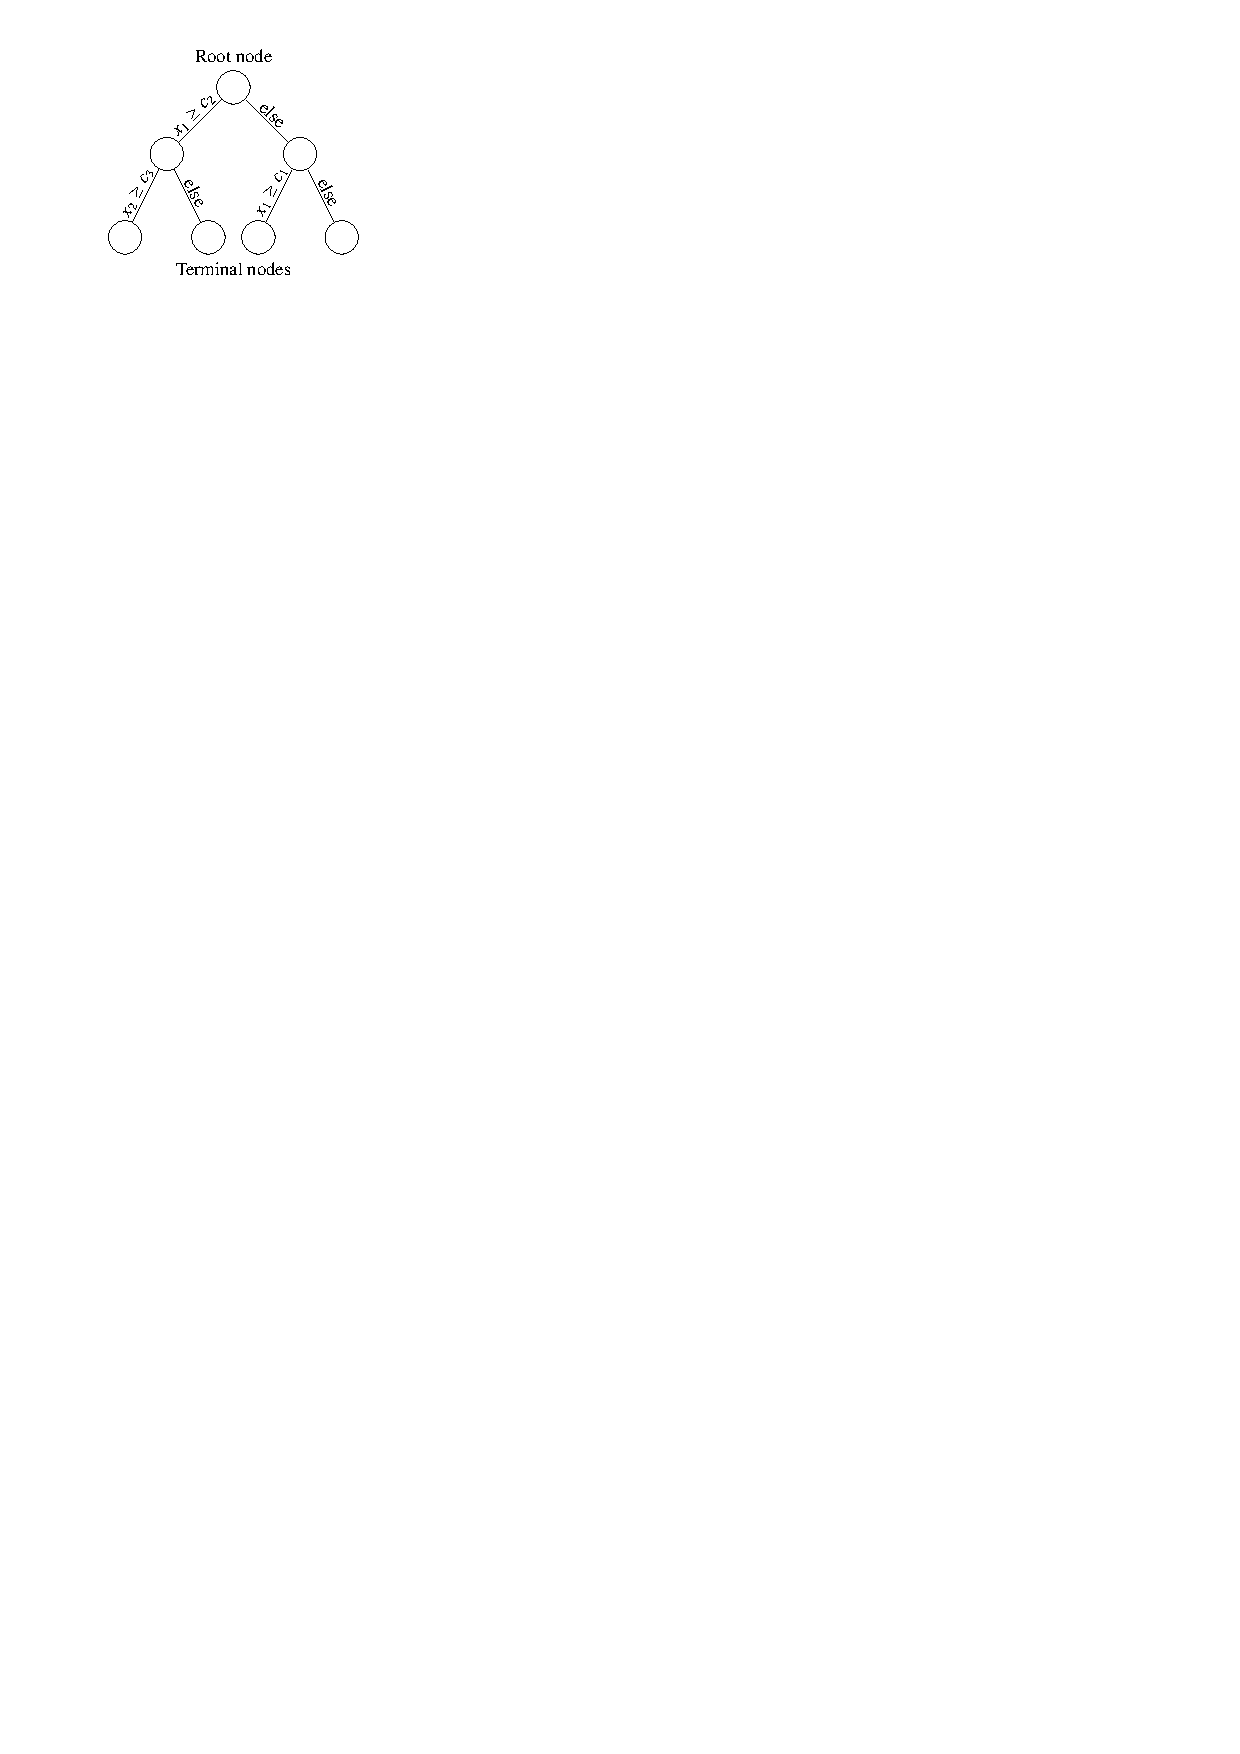
\includegraphics{./figures/theory/decision_tree.pdf}
    \subcaption{Binary tree structure of decision trees.}
    \label{fig:decision_tree_binary_tree}
  \end{subfigure}\hspace*{2em}
  \begin{subfigure}[t]{0.4\textwidth}
    \centering
    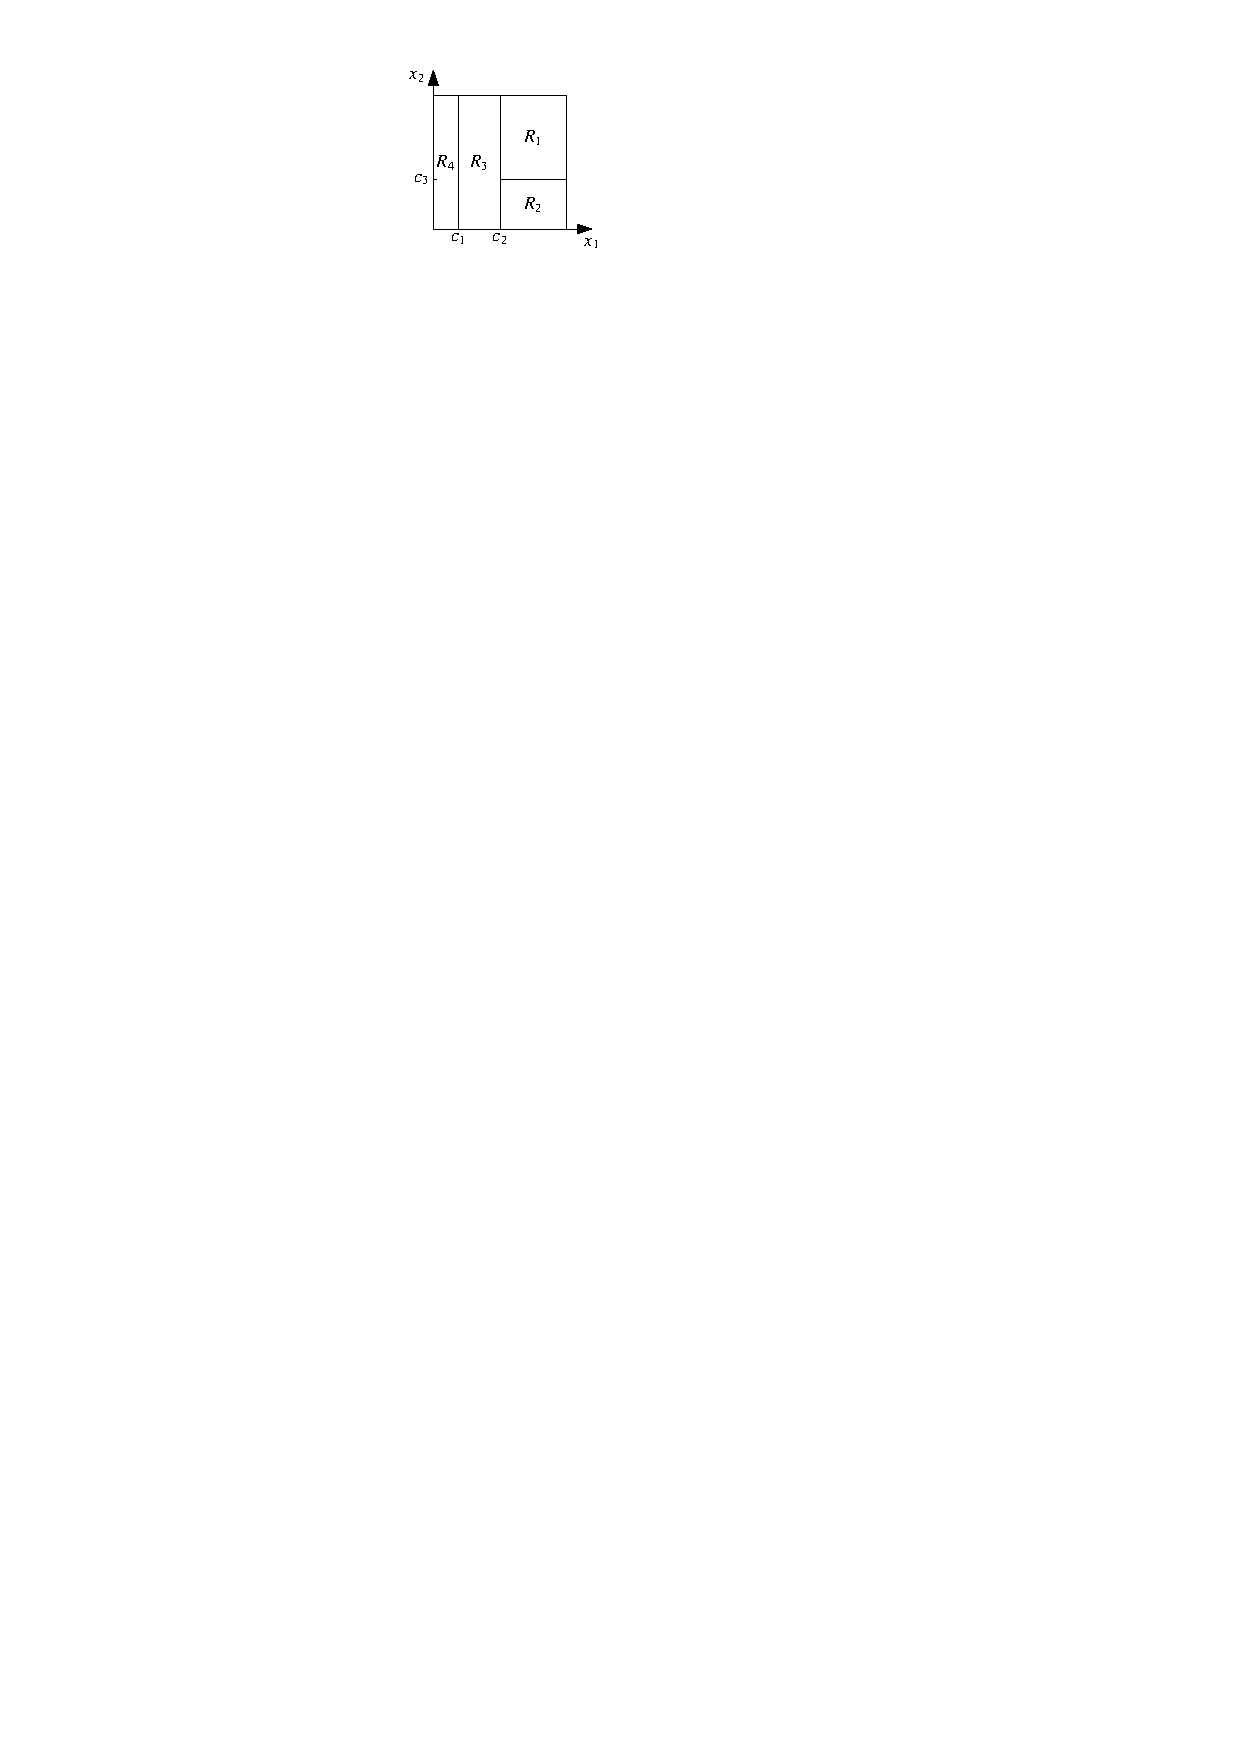
\includegraphics{./figures/theory/decision_tree_partition.pdf}
    \subcaption{Partitioning of the space spanned by the input variables $x_1$
      and $x_2$ into subregions~$R_i$.}
    \label{fig:decision_tree_partition}
  \end{subfigure}
  \caption[Structure of a decision tree]{Structure of a decision tree with
    depth~$d_\text{tree} = 2$ and two input variables $x_1$, $x_2$. Adapted from
    Ref.~\cite{esl}.}
  \label{fig:decision_tree}
\end{figure}

A decision tree is a tree-based model that recursively partitions the space
spanned by the input variables into disjoint subregions by applying binary
splits on the coordinate axes until a stopping criterion is met. Frequently used
criteria include limiting the maximum depth of the tree or requiring a minimum
number of training examples in a subregion considered for further splitting.
Figure~\ref{fig:decision_tree_binary_tree} shows the binary tree structure of a
decision tree. The root node of the tree contains the entire dataset which is
subsequently split into two nodes by a condition on a single input variable. The
terminal nodes contain disjoint subsamples of the dataset with input variables
falling into the distinct regions of the variable space depicted in
Figure~\ref{fig:decision_tree_partition}. Events falling into a subregion are
assigned the probability of being signal given by the fraction of signal events
(i.e.\ the signal purity) of the training data in this region.
% Each terminal node is assigned the
% majority class of the subset of training data contained within it. An
% alternative method to gauge the confidence of the decision is to assign the
% signal purity.
% The subregions of the variable space defined by the terminal nodes Formally:
% majority class minimises classification error, signal purity minimises
% log-loss

A decision tree is grown using a greedy optimisation method, where each node is
split on the variable and value that gives the largest improvement according to
a chosen impurity measure. Commonly used for binary classification trees is the
Gini impurity given by
\begin{align*}
  I_\text{G}(p) = 2 p (1 - p)
\end{align*}
where $p$ is the signal or background purity~\cite{esl}. The best split is
chosen such that the mean of the Gini impurities of the resulting nodes,
weighted by the sum of event weights in each node, is minimised.
% Gini index: Probability to assign the correct label to a randommly picked
% observation when randomly assigning according to the distribution of labels in
% the sample

\subsection{Boosting}
\label{sec:ml_boosting}

Boosting describes a family of machine learning meta-algorithms that are used to
build ensembles of a base learner, aiming to improve the overall predictive
power compared to a single model. The ensembles can be viewed as an additive
expansion in a set of basis functions given by the base learner \cite{esl}.
Boosting is commonly used in conjunction with decision trees giving rise to so
called Boosted Decision Trees.

Adaptive Boosting (AdaBoost) is a boosting algorithm that forms a weighted sum
of a base classifier, where each classifier is trained on data that is
reweighted such that training examples that were previously incorrectly
classified contribute with larger weight than examples that were correctly
classified. A generalisation of this method is called Gradient Boosting which
minimises the expected value of an arbitrary differential loss function, which
is a function penalising errors of the model, during boosting. Gradient Boosting
reproduces the AdaBoost algorithm if the exponential loss function
\begin{align*}
  L\left(y, f(\mathbf{x})\right) = \exp\left(- y f(\mathbf{x})\right)
\end{align*}
with input variables $\mathbf{x}$ of the training example, the true class
encoded as~$y \in \{ -1, 1 \}$ and the model
response~$f(\mathbf{x}) \in [-1, 1]$, is used~\cite{esl}. For general loss
functions no convenient methods for minimising the loss exist and a gradient
descent algorithm is used. A full mathematical description of the algorithm is
omitted and can be found in Refs.~\cite{friedman_gbm, esl}. In this thesis
gradient boosting with the loss function
\begin{align*}
  L\left(y, f(\mathbf{x})\right) = \log\left( 1 + \exp(- 2 y f(\mathbf{x})) \right)\eqcomma
\end{align*}
is used, which is empirically shown to be less susceptible to noise and
outliers, i.e.\ examples with large negative margins~$y f(\mathbf{x})$, than
\emph{AdaBoost} \cite{esl, schapire_boosting}.
% The reason is that the
% exponential loss applies a larger penalty to training examples with large
% negative margins~$y f(x)$, e.g.\ outliers.
%
% (called \emph{LogitBoost}~\cite{logitboost})

\section{Artificial Neural Networks}
\label{sec:nn}

Artificial neural networks encompass a large set of models that can be used as
approximations to a wide variety of nonlinear functions~\cite{hornik}. They can
be thought of as rules to compute a
mapping~\mbox{$\mathbb{R}^n \rightarrow \mathbb{R}^m$} between a set of
$n$~input variables and $m$~desired responses. The central idea is to repeatedly
compute intermediate representations of the inputs by applying transformations
and combining the final representation in a linear or logistic regression model.
Neural networks are typically organised into different layers defining the
transformation that is applied on the layer inputs. Multiple layers connected
according to a computational graph form a network. This scheme allows for great
flexibility in building different models making neural networks prevalent in
many areas of machine learning research~\cite{goodfellow_dl}.

The following sections introduce concepts needed to understand the models used
for the classification tasks in this thesis. Matrices are denoted using
uppercase and vectors using lowercase bold symbols, e.g.\ input
variables~$\mathbf{x}$ and weight matrices~$\mathbf{W}$.

\subsection{Feedforward Neural Networks}
\label{sec:nn_feedforward}
Feedforward neural networks are networks in which information flows strictly in
the forward direction, disallowing feedback loops between input and output of a
single layer. An example of simple feedforward neural networks are the so called
multi-layer perceptrons. They consist of a number of input neurons $\mathbf{x}$,
which are used to pass the discriminating variables to the network, and an
output layer with neuron activations~$\mathbf{y}$ after applying a nonlinear
activation function to the values of the neurons. The input and output layers
are connected by one or more intermediate hidden layers.
\begin{figure}[htb]
  \centering
  \begin{minipage}[t]{0.55\textwidth}
    \centering
    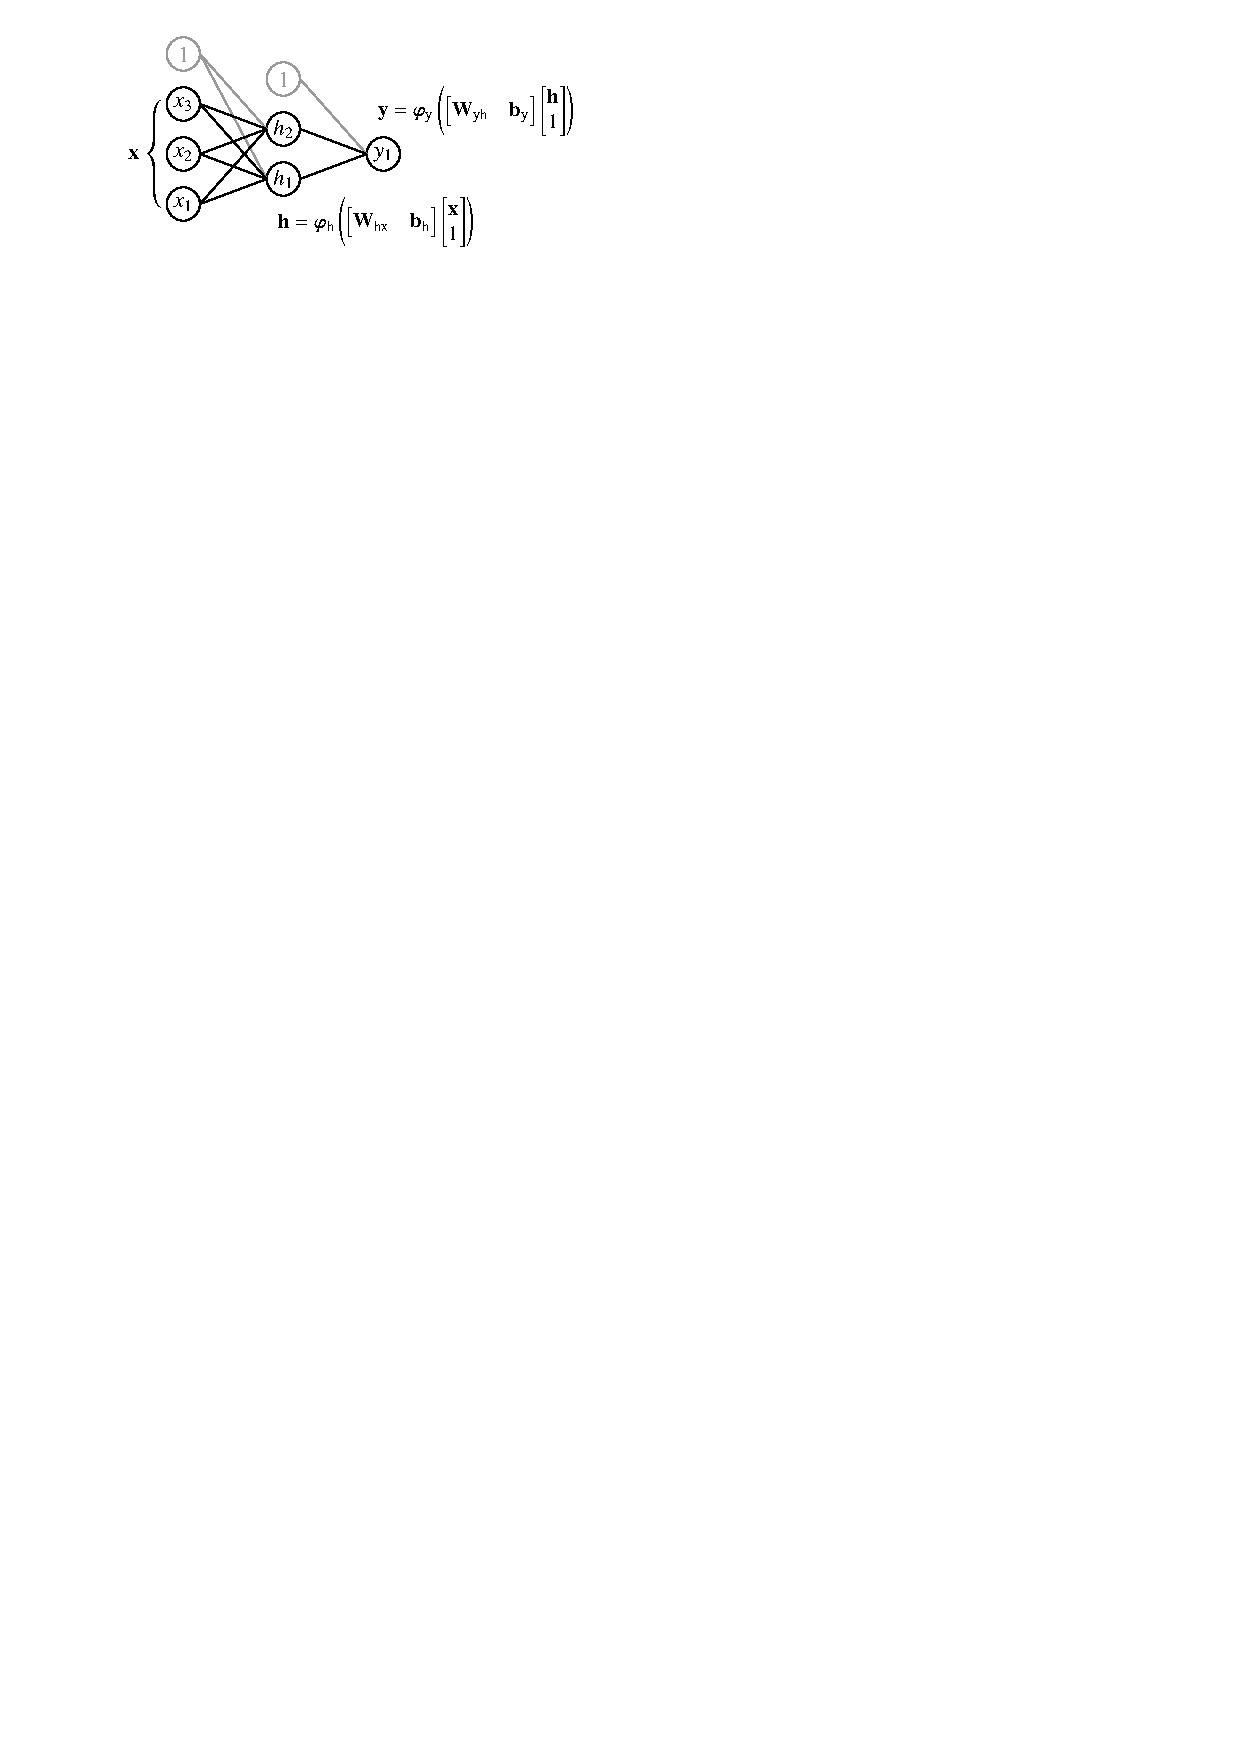
\includegraphics{./figures/theory/mlp.pdf}
    \captionof{figure}[Multi-layer perceptron]{Multi-layer perceptron with
      input layer~$\mathbf{x}$, hidden layer~$\mathbf{h}$ and output
      layer~$\mathbf{y}$. Activations are given after applying an element-wise
      activation function~$\bm{\varphi}$. Block matrix notation is used to
      indicate how biases~$\mathbf{b}$ can be absorbed into a single weight
      matrix.}
    \label{fig:multi_layer_perceptron}
  \end{minipage}\hfill
  \begin{minipage}[t]{0.4\textwidth}
    \centering
    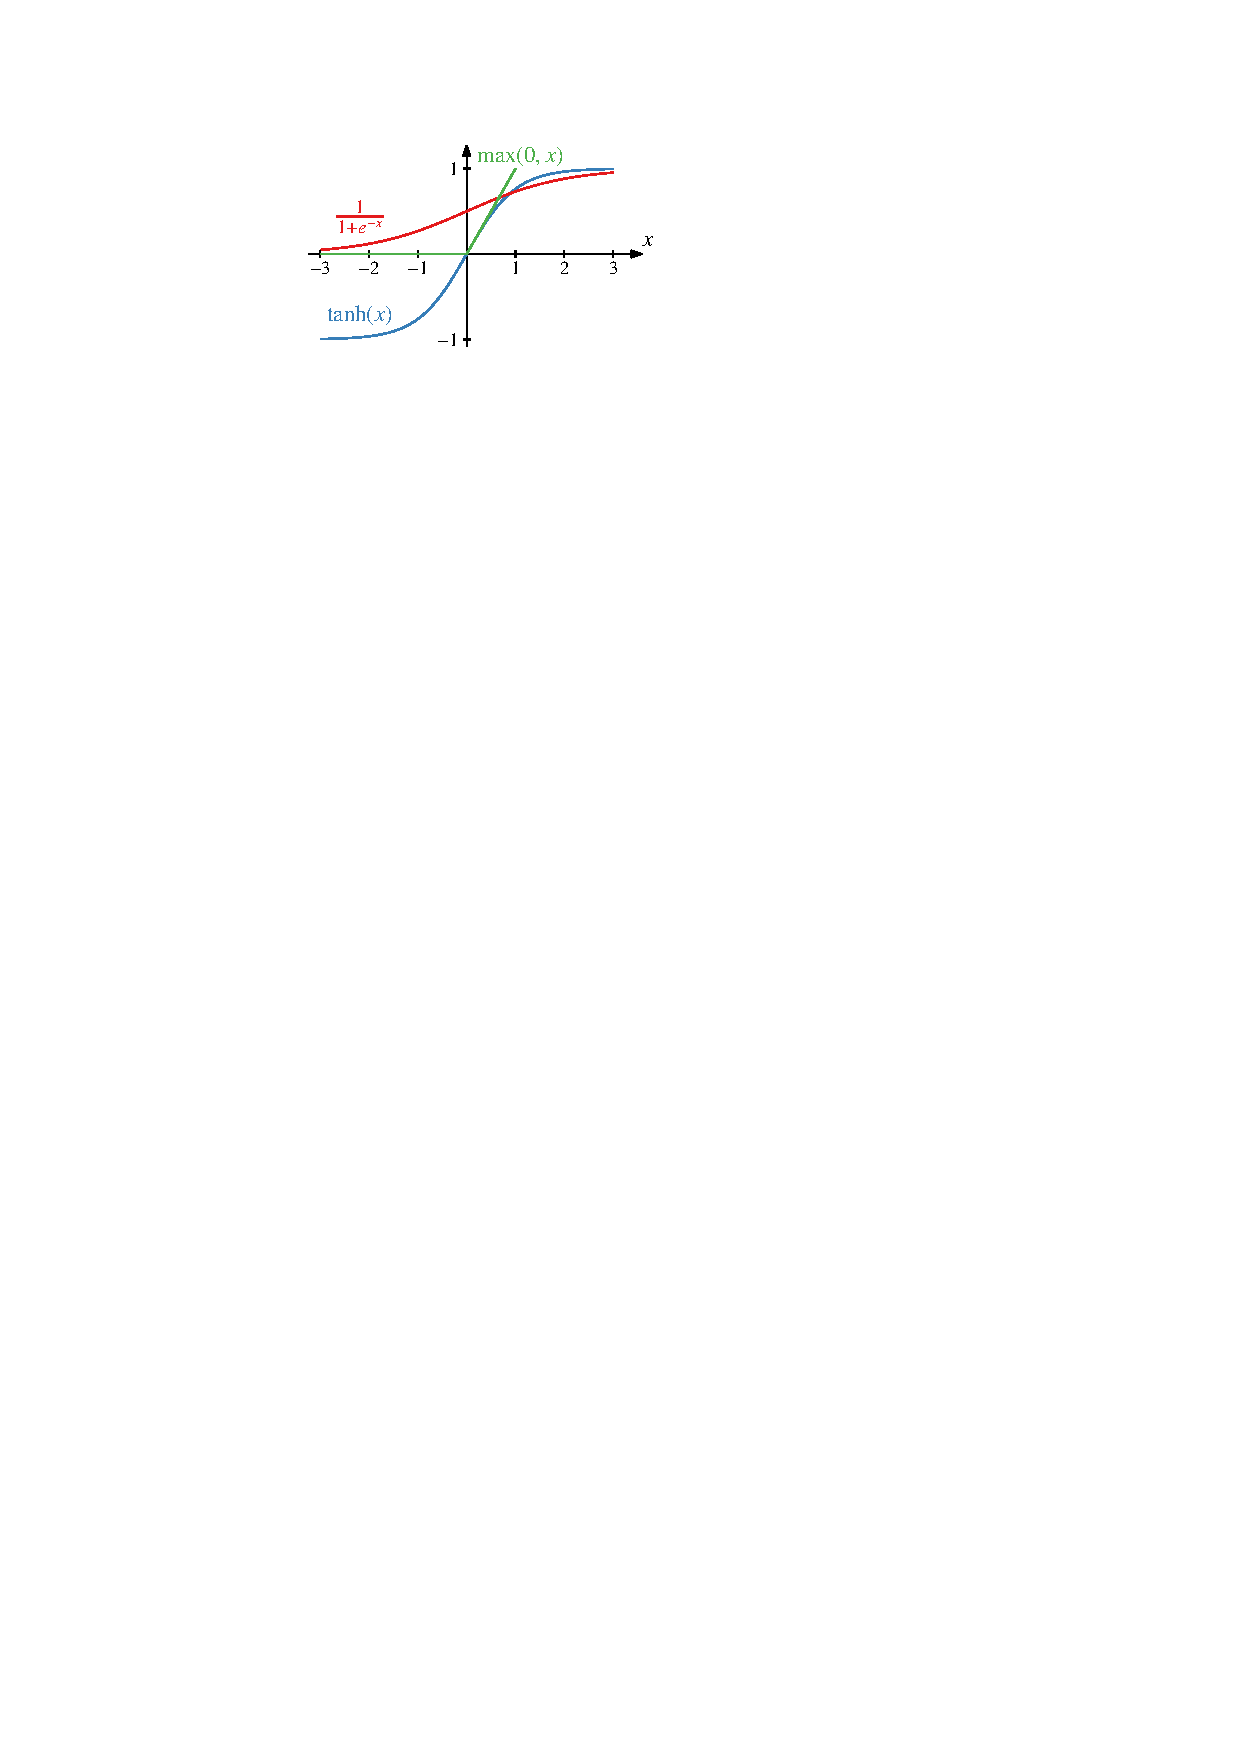
\includegraphics{./figures/theory/activation_functions.pdf}
    \captionof{figure}[Activation functions]{Commonly used activation
      functions: logistic function (red), hyperbolic tangent (blue) and
      rectified linear unit (green).}
    \label{fig:activation_functions}
  \end{minipage}
\end{figure}
In Figure~\ref{fig:multi_layer_perceptron} a multi-layer perceptron with a
single hidden layer is shown. Two layers are connected by an affine
transformation and subsequent application of an element-wise, nonlinear and
differentiable activation function~$\bm{\varphi}$. These layers are called dense
or densely-connected layers, as each neuron is connected to every other neuron
in the neighboring layer. The weight of each connection between two neurons is
determined by weight matrices~$\mathbf{W}$.
% \begin{align*}
%   &\mathbf{h} = \bm{\varphi}_{\text{h}}(\mathbf{W}_{\text{hx}} \mathbf{x} + \mathbf{b}_{\text{h}})
%   &\mathbf{y} = \bm{\varphi}_{\text{y}}(\mathbf{W}_{\text{yh}} \mathbf{h} + \mathbf{b}_{\text{y}}) \eqcomma
% \end{align*}
The number of neurons in the hidden layers as well as activation functions are
hyperparameters, which are parameters that have to be set prior to training of
the model. The sizes of the input and output layers are constrained by the
number of input variables and the number of desired outputs, respectively.
Moreover, the activation function of the output layer is constrained by the
underlying task. For binary classification the logistic function
\begin{align*}
  \sigma(x) = \frac{1}{1 + e^{-x}}
\end{align*}
is applied to a single output neuron~$x$ giving the probability of an event
being of the positive class (e.g.\ signal). For multi-class classification the
number of output neurons is chosen to equal the number of classes to be
distinguished and the softmax function \cite{esl, bishop}
\begin{align*}
  \varphi_i(\mathbf{x}) = \frac{e^{x_i}}{\sum_j e^{x_j}}
\end{align*}
is chosen as the activation function, where~$\varphi_i(\mathbf{x})$ is the
activation of the $i$-th neuron and $x_i$ its value before activation. The
softmax function ensures that the sum of all activations in a layer equals to
one, such that they can be interpreted as class probabilities. Activation
functions that are commonly used for the intermediate layers are depicted in
Figure~\ref{fig:activation_functions}.

Thus far, neural networks are viewed as nonlinear parametric functions mapping
input variables~$\mathbf{x}$ to a response~$\mathbf{y}$ without regarding the
choice of parameters (i.e.\ weights and biases of each layer). The model
parameters are determined using gradient descent by minimising an objective
function (training of the model). The objective function penalises errors in the
predictions of the model and is commonly called the loss function. Categorical
cross-entropy is generally used for multi-class classification differentiating
between $K$~classes. For an event belonging to a class~$k \in \{1, \dots, K\}$
it is defined as \cite{esl, bishop}
\begin{align*}
  L\left(k, \mathbf{p}(\mathbf{x}) \right) = - \log\left( p_k(\mathbf{x}) \right) \eqcomma
\end{align*}
where~$\mathbf{p}(\mathbf{x}) = \mathbf{y}(\mathbf{x})$ is the probabilistic
interpretation of the model with class probabilities~$p_k$ after softmax
activation and discriminating variables~$\mathbf{x}$. For binary classification
it is sufficient to give the predicted probability~$p$ for the positive class
such that the binary cross-entropy can be written as
\begin{align*}
  L(t, p(\mathbf{x})) = -t \, \log(p(\mathbf{x})) - (1 - t) \, \log(1 - p(\mathbf{x})) \eqcomma
\end{align*}
with the binary indicator~$t$ encoding the true class (0 for the negative and 1
for the positive class). For a subset of events with weights~$w_i$ the
loss~$\mathcal{L}$ is defined as
\begin{align*}
  &\mathcal{L} = \frac{\sum_i w_i L_i}{\sum_j w_j}
    \qquad \text{with} \qquad
    L_i = L\left(k_i, \mathbf{p}(\mathbf{x}_i)\right) \eqdot
\end{align*}
In case of the cross-entropy $\mathcal{L}$ can be interpreted as the negative
log-likelihood of the network parameters given the observed subset of data and
assuming the distribution of classes follows a (generalised) \textsc{Bernoulli}
distribution \cite{bishop}.

The task of finding the parameters of the model minimising the expected loss on
a set of training data is solved using stochastic gradient descent. This
requires information on the gradient of the loss~$\mathcal{L}(\bm{\theta})$ with
respect to the model parameters~$\bm{\theta}$, while keeping the training
examples fixed. Each layer in the computational graph making up the network has
a well-defined derivative such that by repeatedly applying the chain rule for
partial derivatives the gradient $\nabla_{\bm{\theta}} \mathcal{L}(\bm{\theta})$
can be calculated symbolically. This procedure is generally known as error
backpropagation~\cite{bishop, lecun-backprop}. Knowing the gradient of the loss
an iterative optimisation method called mini-batch stochastic\footnote{The
  gradient of the loss on the full training sample is approximated by the
  gradient on a mini-batch.} gradient descent is employed. Initially the weights
are randomised to small values and biases set to zero. The set of training
examples is divided into subsets of fixed size called mini-batches. In an
iterative procedure the parameters are updated according to
\begin{align*}
  \bm{\theta}_{t+1} = \bm{\theta}_t - \eta \, \nabla_{\bm{\theta}} \mathcal{L}(\bm{\theta}_t) \eqcomma
\end{align*}
where $\eta > 0$ is called the learning rate and
$\nabla_{\bm{\theta}} \mathcal{L}(\bm{\theta}_t)$ is the gradient evaluated on
the mini-batch. One pass over all mini-batches is called an epoch and typically
multiple epochs are required to train a model. In practice, the loss on an
independent validation set is observed and the procedure is stopped when the
validation loss stops decreasing.
% \todo[inline]{Find more references; Large penalties to predictions that are far
%   off; Perfect classifiers have loss of zero (can always be reached with complex
%   models); Cross validation?}

\subsection{Recurrent Neural Networks}
\label{sec:rnn_theory}
Events reconstructed in particle detectors can contain a variable number of
reconstructed objects of the same type e.g.\ particle tracks or clusters in the
calorimeter. The rigid structure of feedforward neural networks does not offer a
general method to classify events with variable numbers of objects. Recurrent
neural networks~(RNN) provide an approach to sequence classification by
introducing so called cyclical connections within layers in which units are
connected to themselves. These recurrent connections allow decisions to be made
in the context of the sequence (e.g.\ obeying constraints due to momentum
conservation) by making the network able to store information on previous
objects \cite{graves}.

The \textsc{Elman} network is introduced and will be extended to the long
short-term memory~(LSTM) architecture used in this thesis. Biases are omitted in
the following description as they can be absorbed into the weight matrices.

\subsubsection{Simple Recurrent Networks}
\label{sec:simple_recurrent_networks}
\begin{figure}[htb]
  \centering
  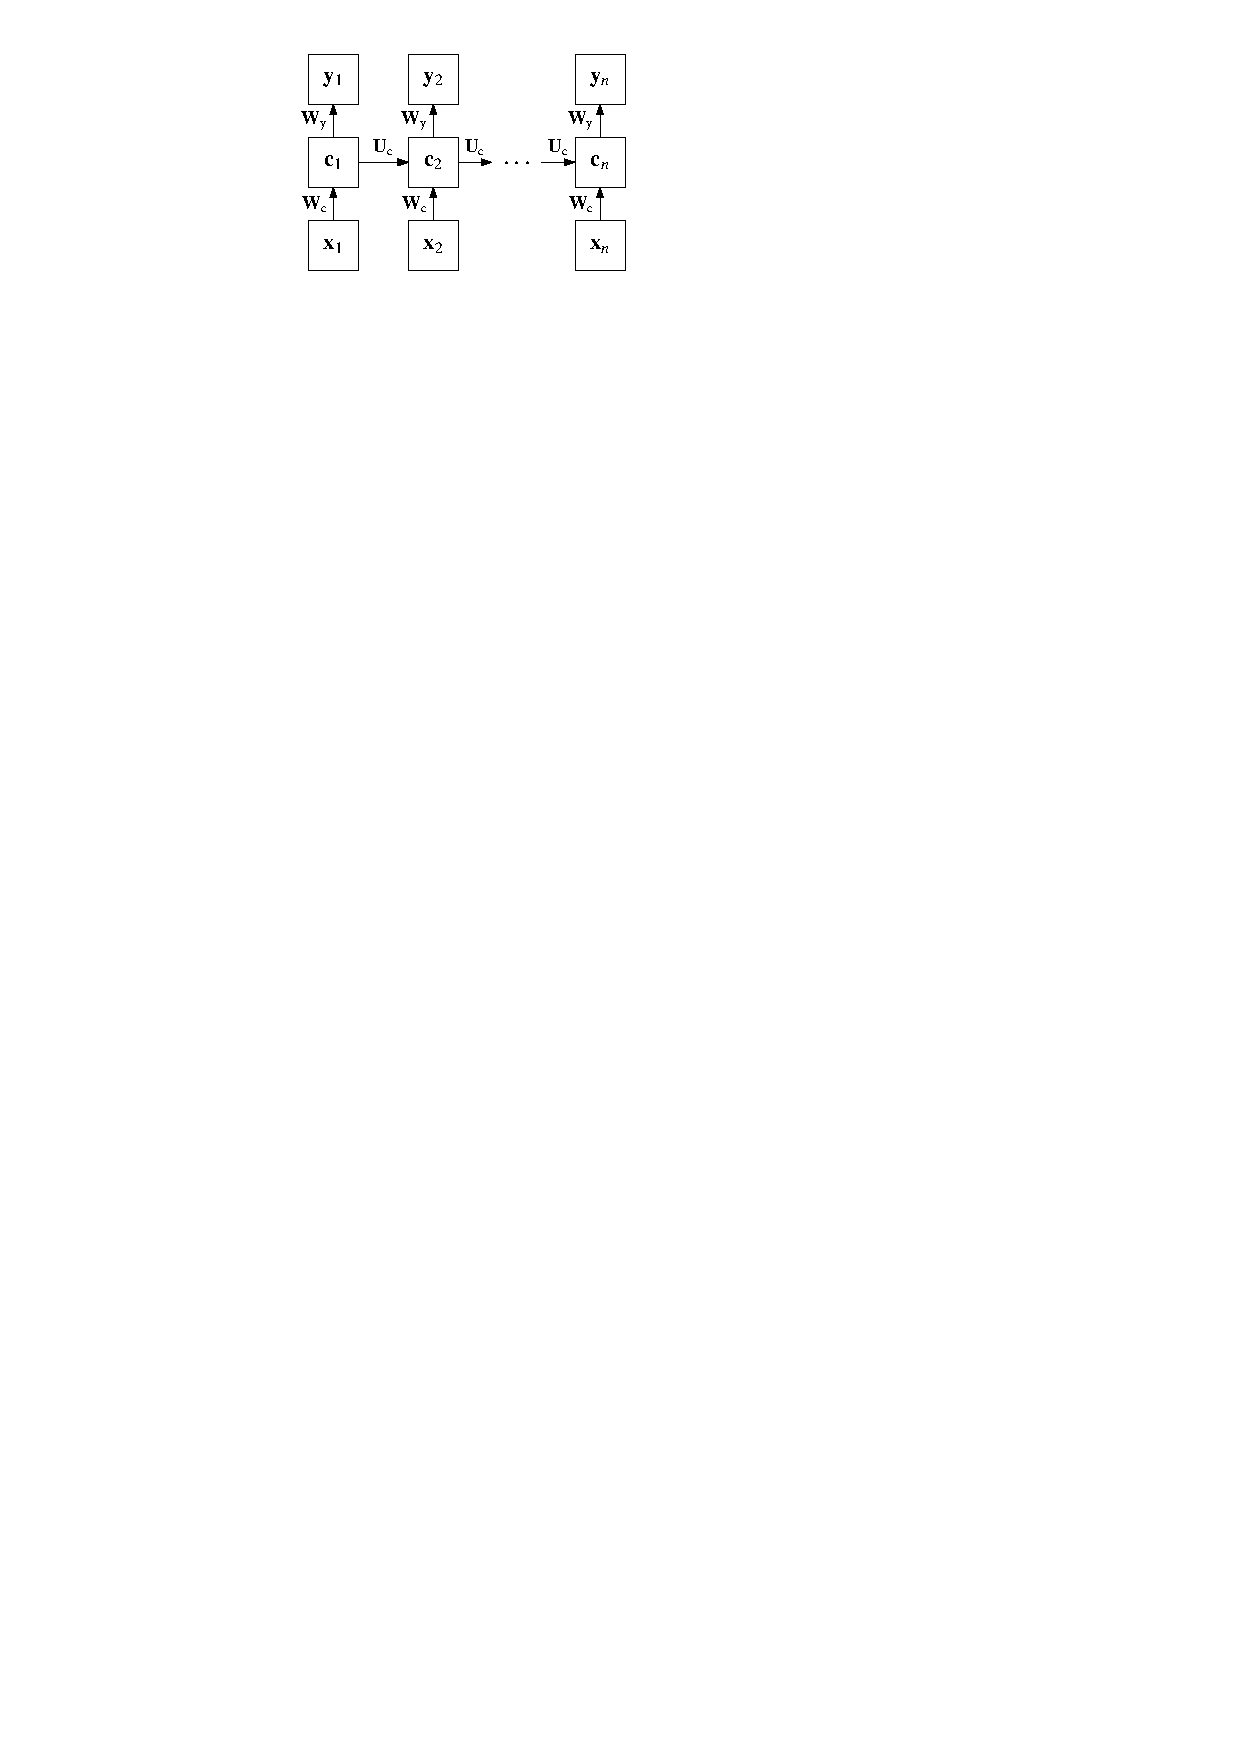
\includegraphics{./figures/theory/elman_rnn.pdf}
  \caption[\textsc{Elman} network]{\textsc{Elman} network in compact form with
    a recurrent connection and after unfolding the network in time. The black
    square indicates a delay of one time step. Applications of nonlinear
    activation functions are omitted. Adapted from
    Ref.~\cite{lecun_bengio_hinton_DL}.}
  \label{fig:schematic_elman_rnn}
  %\footnote{Nomenclature originates from RNNs being used to predict quantities as a function of time.}
\end{figure}

Recurrent neural networks are able to map a sequence of input variables to a
sequence of outputs. Both sequences can contain an arbitrary number of objects.
An example of a Simple Recurrent Network is the \textsc{Elman}
network~\cite{elman} depicted in Figure~\ref{fig:schematic_elman_rnn}. After
unfolding the network in time it can be represented as a feedforward network
with weights shared between time steps. The input
sequence~$\left( \mathbf{x}_i \right)_{i=1}^n$ is processed one element at a
time. The sequence of cell states~$\mathbf{c}_t$ and outputs~$\mathbf{y}_t$ are
computed by iteratively applying the rule
\begin{align*}
  \mathbf{c}_t &= \bm{\varphi}_{\text{c}}\Big( \mathbf{W}_{\text{c}} \mathbf{x}_{t} + \mathbf{U}_{\text{c}} \mathbf{y}_{t-1} \Big)
  &\mathbf{y}_t &= \bm{\varphi}_{\text{y}}\Big( \mathbf{W}_{\text{y}} \mathbf{c}_{t} \Big)
\end{align*}
with weights~$\mathbf{W}$, recurrent weights~$\mathbf{U}$ and activation
functions~$\bm{\varphi}$, while incrementing the time step~$t$~\cite{elman,
  graves}. The initial cell state is often set to $\mathbf{c}_0 = \mathbf{0}$
but the particular choice can differ between implementations. All weights are
shared between time steps, which allows sequences of arbitrary length to be
processed by the network. The cell state~$\mathbf{c}_t$ at each time step~$t$ is
updated using the external input~$\mathbf{x}_t$ as well as the cell
state~$\mathbf{c}_{t-1}$ of the previous time step, forming the recurrent
connection. This allows a memory of previous inputs to persist in the internal
state of the network, thus enabling the output~$\mathbf{y}_t$ to depend on the
history of the sequence. As Simple Recurrent Networks process the input sequence
in a predefined direction, only the past information can influence the output at
a specific time step, making the order of the input sequence important. An
architecture allowing the context (past and future) to influence the output at a
given time~$t$ are so called bidirectional RNNs.

The evaluation of the gradient for the training process follows the same
principles used for feedforward neural networks but now also considering that
the chain rule has to be applied for each time step and that the weights between
time steps are shared (called backpropagation through
time~\cite{williams_zipser}). After unfolding the network in time, the training
is analogous to that of feedforward neural networks.

In this thesis RNNs are used for the classification of a sequence of
reconstructed objects in its entirety as opposed to classifying each element in
the sequence. For this task the full output sequence of the recurrent network is
not needed, such that only the output of the last time step is used. Simple
Recurrent Networks like the \textsc{Elman} network show that the gradient signal
decays with each time step making it difficult to learn structure spanning over
multiple time steps in the input sequence. This is known as the vanishing
gradient problem~\cite{hochreiter, lecun_bengio_hinton_DL}. The following
section will present an extension to this architecture enabling the network to
learn long-term dependencies.
% \todo{This is due to the repeated
%   application of the activation function e.g.\ $\tanh$ in the recurrent
%   connection leading to a exponential decay of the gradient -- also affects
%   feedforward networks}.

\subsubsection{Long Short-Term Memory}
\label{sec:lstm}
The long short-term memory (LSTM) network developed in Ref.~\cite{lstm} solves
the vanishing gradient problem by introducing multiplicative gates, which
perform an element-wise multiplication of gate activations and inputs, thereby
controlling the flow of information in the network. In
Figure~\ref{fig:schematic_lstm} a schematic depiction of an unfolded LSTM at
time~$t$ is shown.
\begin{figure}[htb]
  \centering
  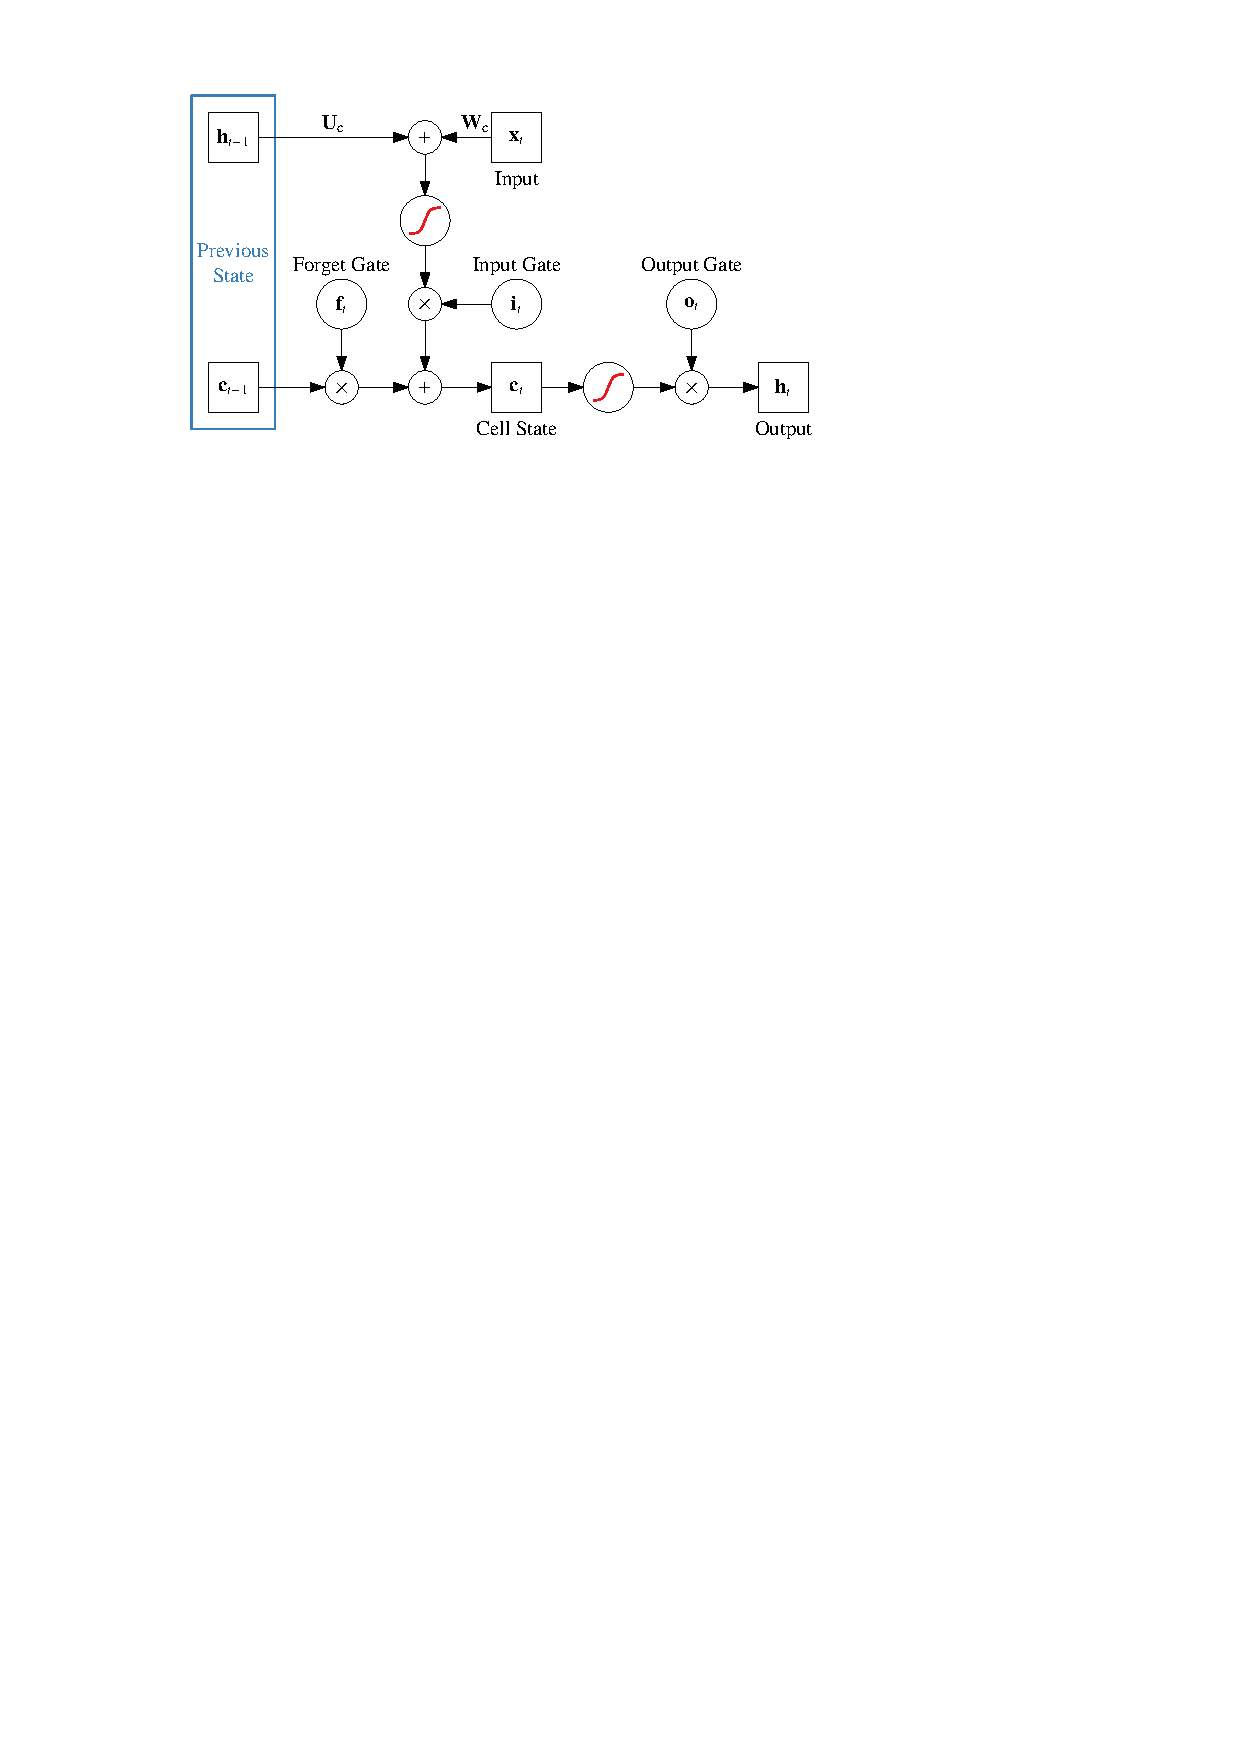
\includegraphics{./figures/theory/LSTM.pdf}
  \caption[LSTM-cell]{LSTM-cell unfolded in time at a fixed time step~$t$. Nodes
    with~$\times$ ($+$) multiply (add) their inputs element-wise, while ones
    containing a sigmoid shape apply a nonlinear activation function. The
    dependency of the gate vectors $\mathbf{i}_t$, $\mathbf{o}_t$ and
    $\mathbf{f}_t$ on input~$\mathbf{x}_t$ and output~$\mathbf{y}_{t-1}$ is
    omitted.}
  \label{fig:schematic_lstm}
\end{figure}
The LSTM represents a differentiable memory cell with three gates called the
input, output and forget gate. The gate vectors, controlling the information
flow, are given by \cite{goodfellow_dl, graves}
\begin{align*}
  \mathbf{i}_{t} &= \bm{\sigma}\left( \mathbf{W}_{\text{i}} \mathbf{x}_{t} + \mathbf{U}_{\text{i}} \mathbf{y}_{t-1} \right) &
  \mathbf{o}_{t} &= \bm{\sigma}\left( \mathbf{W}_{\text{o}} \mathbf{x}_{t} + \mathbf{U}_{\text{o}} \mathbf{y}_{t-1} \right) &
  \mathbf{f}_{t} &= \bm{\sigma}\left( \mathbf{W}_{\text{f}} \mathbf{x}_{t} + \mathbf{U}_{\text{f}} \mathbf{y}_{t-1} \right)
\end{align*}
with separate weights~$\bm{W}$ and recurrent weights~$\bm{U}$ for each gate. The
element-wise logistic function~$\bm{\sigma}$ is used to map the gate activations
into the interval $[0, 1]$. Notably, the gate activations depend on the
input~$\mathbf{x}_t$ at time~$t$ as well as the output~$\mathbf{y}_{t-1}$ of the
LSTM at the previous time step. How the gating controls the flow of information
in an LSTM can be understood by looking at the update of the cell
state~$\mathbf{c}$ with each time step \cite{graves, goodfellow_dl}
\begin{align*}
  \mathbf{c}_{t} &= \mathbf{f}_{t} \circ \mathbf{c}_{t-1}
                   + \mathbf{i}_{t} \circ \bm{\varphi}_{\text{c}}(
                   \mathbf{W}_{\text{c}} \mathbf{x}_{t}+ \mathbf{U}_{\text{c}}
                   \mathbf{y}_{t-1} ) \eqcomma
\end{align*}
where $\circ$ denotes the element-wise product of two column vectors and the
activation function~$\bm{\varphi}_c$ is the hyperbolic tangent in the
implementation \cite{keras} used in this thesis. Similar to the Simple Recurrent
Networks the initial cell state $\mathbf{c}_0$ and output $\mathbf{y}_0$ are set
to $\mathbf{0}$. The input gate controls how much information from the
input~$\mathbf{x}_t$ and previous output~$\mathbf{y}_{t-1}$ is taken into the
cell state, thereby reducing the inclusion of irrelevant information. A main
feature of the LSTM architecture is the direct connection of cell states between
two successive time steps via the forget gate which solves the vanishing
gradient problem~\cite{lstm, graves}. The forget gate enables the network to
gradually reset its internal state once stored information has become
irrelevant. Finally the output~$\mathbf{y}_t$ is calculated using \cite{graves,
  goodfellow_dl}
\begin{align*}
  \mathbf{y}_{t} &= \mathbf{o}_{t} \circ \bm{\varphi}_{\text{y}}(\mathbf{c}_{t}) \eqcomma
\end{align*}
where~$\bm{\varphi}_\text{y}$ is the hyperbolic tangent. The activation of the
output gate determines how much of the cell state is presented at the output of
the network. Overall, the multiplicative gating of the LSTM allows information
to persist in its internal state over a long period of time, with gates
resembling the write, read and reset gates of conventional memory cells.
Alternative architectures to LSTMs exist (e.g.\ Gated Recurrent Units) but were
not investigated in this thesis.

\section{Technical Setup}
\label{sec:tech_setup}

In this thesis the Toolkit for Multivariate Data Analysis~(TMVA)~\cite{tmva} is
used for the BDT-based studies on tau identification in Chapter~\ref{sec:bdt}.
This framework is extensively used for evaluating multivariate algorithms for
the reconstruction of hadronic tau lepton decays in the ATLAS experiment.

The neural network based studies in chapters~\ref{sec:rnn}
and~\ref{sec:decaymode} use the \textsc{keras} framework~\cite{keras} which
offers implementations of commonly used layers (i.e.\ the rules to compute the
forward pass as well as the symbolic derivatives for backpropagation), loss
functions and optimisers. Moreover, it takes care of the necessary bookkeeping
when building neural networks. The \textsc{theano} backend~\cite{theano} is used
in \textsc{keras} performing fast computation of mathematical expressions for
training and evaluation of the networks. For the preprocessing of the data, the
\textsc{numpy} \cite{numpy} and \textsc{scipy} \cite{scipy} packages are used.
The training of the neural networks uses the \textsc{Adam} optimiser~\cite{adam}
which is a stochastic gradient descent algorithm with adaptive learning rates
offering quick convergence with little parameter tuning. The layers used in this
thesis are (\textsc{keras} naming convention): \texttt{Dense} for
densely-connected layers; \texttt{LSTM}; \texttt{Merge} for concatenating
outputs from multiple layers and \texttt{Masking} to skip time steps in
recurrent networks with a predefined default value. The Dense and LSTM layers
use biases which were previously omitted.

%%% Local Variables:
%%% mode: latex
%%% TeX-master: "mythesis"
%%% End:

% ~ 12 pages
\chapter{Identification of Hadronically Decaying $\tau$-Leptons (BDT)}
\label{sec:bdt}

\section{Features of Hadronically Decaying Tau Leptons}
\label{sec:features_tau_decay}

Features of hadronically decaying $\tau$-leptons vs. Quark/Gluon initiated jets:
\begin{itemize}
\item Low multiplicity (QCD jets usually have a lot of tracks)
\item Isolated tracks and narrow showers
\item Measurable decay length with proper lifetime of
  $\tau = \SI{290.3 +- 0.5}{\femto\second}$ \cite{pdg} and following from that
  $c \tau = \SI{87.0 +- 0.2}{\micro\metre}$ with $\beta \gamma = 10$ which
  corresponds to a roughly \SI{18}{\giga\electronvolt} tau the mean decay length
  is of the order of a millimetre and allows secondary vertex reconstruction or
  employing the impact parameter for 1-prong taus (sub-millimetre resolution).
\item Invariant mass bounds for decay products
\end{itemize}


\section{Event Simulation, Reweighting and Preselection}
\label{sec:bdt_eventsim}

\todo{Signal}
For training and performance evaluation simulated data is used. For tau
performance trainings and tunings a sample created by the process
$\gamma^* \rightarrow \tau \tau \, \text{(hadr.)}$ is used, where at
generator-level leptonic decays of the tau is disabled. Moreover interference
with and on-/ off-shell production of the $\mathrm{Z}^0$ boson is disabled. The
reason for not using a sample employing the Drell--Yan process including
interference and on- / off-shell production of the $\mathrm{Z}^0$ boson is that
the tau polarisation changes for di-tau invariant masses close to the
$\mathrm{Z}$-mass whereas unpolarised taus are desired. Moreover the di-tau mass
spectrum is smooth and decreasing without increased statistics close to the
$\mathrm{Z}$ mass which is not needed for performance studies.

\todo{Background} The background for the identification studies is given by
dijet samples up to \SI{1800}{\giga\electronvolt} (JZ1W - JZ6W). \todo{Finish
  this}

Baseline tau selection:
\begin{itemize}
\item $p_\text{T} > \SI{20}{\giga\electronvolt}$ (sufficient for most analyses)
\item Exclude calorimeter transition region $1.37 < |\eta| < 1.52$
\item Require tracker acceptance region $|\eta| < 2.5$
\item One or three reconstructed tracks
\item Truth-matching for signal events ($p_\text{T}$, $\eta$ and
  $N_\text{track}$ selection also at truth-level)
\end{itemize}

Size of the pre-production samples after baseline tau selection:
\begin{itemize}
\item Signal: 13.3 M (1P: 10.5 M, 3P: 2.8 M)
\item Background: 22.1 M (1P: 6.6 M, 3P: 15.5 M)
\end{itemize}

\todo{Interesting plots: pt spectra, mu-distribution}

\todo{Reweighting}

A full summary of the datasets is given in appendix \todo{Reference}.

\section{Description of the Tau-Identification Procedure}
\label{sec:bdt_tauid}

\subsection{Features (Predictors, Dependent Variables, Input Variables)}
\label{sec:bdt_features}

Input variables
\begin{itemize}
\item Central energy fraction $f_\text{cent}$ (1P, 3P)
\item etOverPtLeadTrk $f_\text{leadtrack}^{-1}$ (1P, 3P)
\item innerTrkAvgDist $R_\text{track}^{0.2}$ (1P, 3P)
\item absipSigLeadTrk $\left| S_\text{leadtrack} \right|$ (1P)
\item SumPtTrkFrac $f_\text{iso}^\text{track}$ (1P)
\item ChPiEMEOverCaloEME $f_\text{EM}^\text{track-HAD}$ (1P, 3P)
\item EMPOverTrkSysP $f_\text{track}^\text{EM}$ (1P, 3P)
\item ptRatioEflowApprox $p_\text{T}^\text{EM+track} / p_\text{T}$ (1P, 3P)
\item mEflowApprox $m_\text{EM+track}$ (1P, 3P)
\item dRmax $\Delta R_\text{max}$ (3P)
\item trFlightPathSig $S_\text{T}^\text{flight}$ (3P)
\item massTrkSys $m_\text{track}$ (3P)
\end{itemize}

Setup
\begin{itemize}
\item NTrees: 100
\item MaxDepth: 8
\item AdaBoostBeta: 0.2
\item MinNodeSize: 0.1
\item nCuts: 200
\item UseYesNoLeaf: False
\item PruneMethod: NoPruning
\end{itemize}
Previous setup (incl. explanation \& plots of input variables)

Transformations? highly skewed and long-tailed distributions

\section{Hyperparameter Optimisation}
\label{sec:bdt_hyperparam}

TMVA \cite{tmva}.

Quickly describe previous setup.

Before proceeding to feature selection a reliable hyperparameter setup has to be
found.

Pick the best-performing BDT \& a good compromise between 'overtraining' and
performance.

Optimised for tight efficiency w/o subsampling:
\begin{itemize}
\item \textbf{Best performance 1P:} MaxDepth: 16, MinNodeSize: 0.01, NTrees:
  400, Shrinkage: 0.05, ratio: 0.997 \textrightarrow alg 244
\item \textbf{Compromise 1P:} MaxDepth: 8, MinNodeSize: 0.1, NTrees: 400,
  Shrinkage: 0.1, sumsampling: 50\%, ratio: 0.977 \textrightarrow alg 321
\item \textbf{Best performance 3P:} MaxDepth: 16, MinNodeSize: 0.01, NTrees:
  400, Shrinkage: 0.4, ratio: 0.998 \textrightarrow 259
\item \textbf{Compromise 3P:} MaxDepth: 6, MinNodeSize: 0.1, NTrees: 800,
  Shrinkage: 0.4, ratio: 0.964 \textrightarrow alg 327
\end{itemize}

\subsection{Boosting Algorithm}
\label{sec:bdt_boosting}
AdaBoost \textrightarrow GradBoost

\begin{figure}[ht]
  \begin{subfigure}[t]{0.48\textwidth}
    \centering
    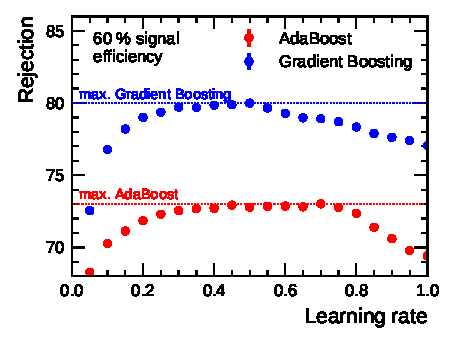
\includegraphics{./figures/bdt_perf/boosting.pdf}
    \subcaption{Impact of the boosting algorithm. $N_\text{trees} = 100$,
      $d_\text{tree} = 8$, $f_\text{node}^\text{min} = \SI{0.1}{\percent}$ and
      varying the learning rate $\beta$~(\emph{AdaBoost}) and $\eta$~(Gradient
      Boosting) respectively.}
    \label{fig:bdt_boosting_alg}
  \end{subfigure}\hfill
  \begin{subfigure}[t]{0.48\textwidth}
    \centering
    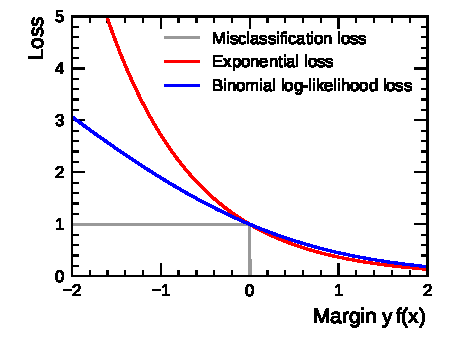
\includegraphics{./figures/theory/boosting_loss.pdf}
    \subcaption{Loss function vs.\ margin \cite{esl}}
    \label{fig:boosting_loss}
  \end{subfigure}
  \caption{Loss function investigation}
\end{figure}

\todo{Plot of the 'margin' $y f(x)$ for exponential and binomial log-likelihood?}

\subsection{Exhaustive Grid Search}
\label{sec:bdt_grid_search}

\begin{align*}
  N_\mathrm{trees} &\in \{25, 50, 100, 200, 400, 800\} &
  d_\mathrm{tree} &\in \{4, 6, 8, 12, 16\} \\
  \eta &\in \{0.05, 0.1, 0.2, 0.4\} &
  f_\mathrm{node}^\mathrm{min} &\in \{\SI{0.01}{\percent}, \SI{0.1}{\percent},\SI{1.0}{\percent}\} \\
  f_\text{bag} &\in \{\text{None}, \SI{50}{\percent} \}
\end{align*}
Total of $6 \times 5 \times 4 \times 3 \times 2 = 720$

Explain why for 1-prong a subsampling model is better than for 3-prong. The
1-prong case seems to be limited by background statistics while the 3-prong case
is limited by signal statistics. Could the reason for the preferred subsampling
models in the 1-prong case be the low statistics for the background? Why?

Reasons for using the 'less overtrained' example:
\begin{itemize}
\item More robust to potential decreases in number of training examples for
  future tunings
\item BDT fits statistical fluctuations (why is this bad when we see an overall
  improvement in performance? how does this fit in with the NN studies where
  this is often the case?)
\end{itemize}

TMVA Grid Search
XGBoost (?)
Comparison with previous setup

\begin{figure}[ht]
  \begin{subfigure}[t]{0.48\textwidth}
    \centering
    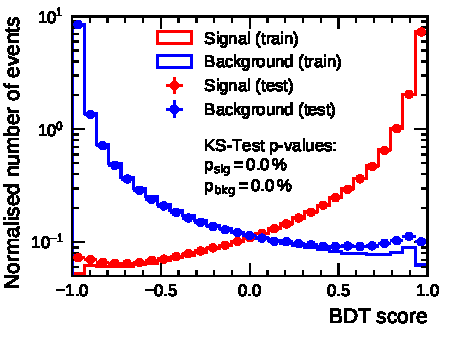
\includegraphics{./figures/bdt_perf/scores/grid_1p0304.pdf}
    \subcaption{Overtrained example (BDT A):
      \mbox{$N_\text{Trees} = 800$},
      \mbox{$d_\text{Tree} = 16$},
      \mbox{$\nu = 0.05$, $f_\text{min.}^\text{Node} = \SI{0.01}{\percent}$},
      no bagging
    }
  \end{subfigure}\hfill
  \begin{subfigure}[t]{0.48\textwidth}
    \centering
    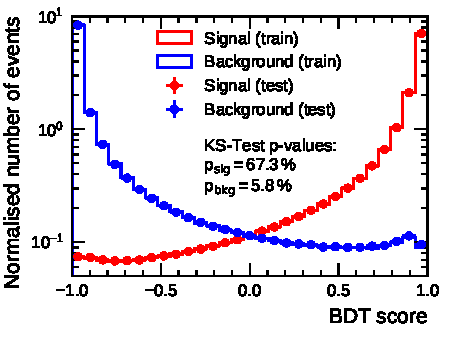
\includegraphics{./figures/bdt_perf/scores/grid_1p_subsampling0269.pdf}
    \subcaption{Good training (BDT B):
      \mbox{$N_\text{Trees} = 400$},
      \mbox{$d_\text{Tree} = 8$},
      \mbox{$\nu = 0.1$, $f_\text{min}^\text{Node} = \SI{0.1}{\percent}$},
      \mbox{$f_\text{bag} = \SI{50}{\percent}$}
    }
  \end{subfigure}
  \caption{'Overtraining' visible on the edges of the BDT score distribution}
  \label{fig:bdt_1p_scores}
\end{figure}

\begin{figure}[ht]
  \begin{subfigure}[t]{0.48\textwidth}
    \centering
    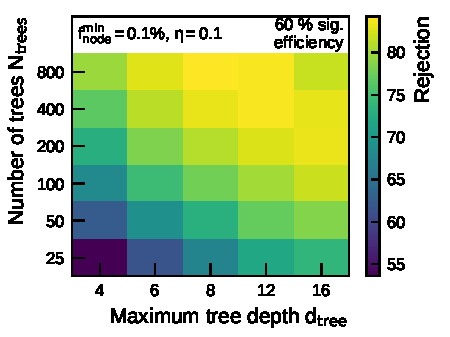
\includegraphics{./figures/bdt_perf/gridsearch_1p/scan_MaxDepth_NTrees.pdf}
    \subcaption{Bla}
  \end{subfigure}\hfill
  \begin{subfigure}[t]{0.48\textwidth}
    \centering
    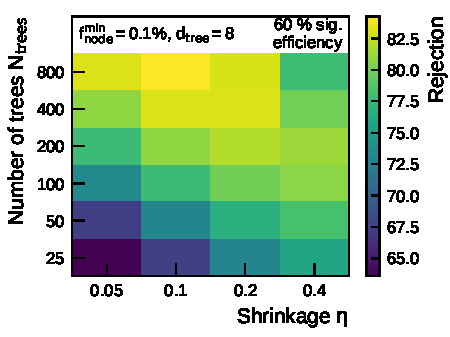
\includegraphics{./figures/bdt_perf/gridsearch_1p/scan_Shrinkage_NTrees.pdf}
    \subcaption{Blabla}
  \end{subfigure}
  \begin{subfigure}[t]{0.48\textwidth}
    \centering
    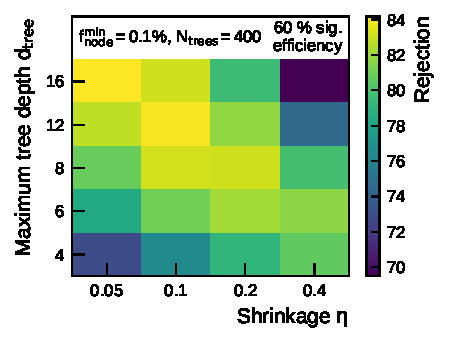
\includegraphics{./figures/bdt_perf/gridsearch_1p/scan_Shrinkage_MaxDepth.pdf}
    \subcaption{Blablabla}
  \end{subfigure}\hfill
  \begin{subfigure}[t]{0.48\textwidth}
    \centering
    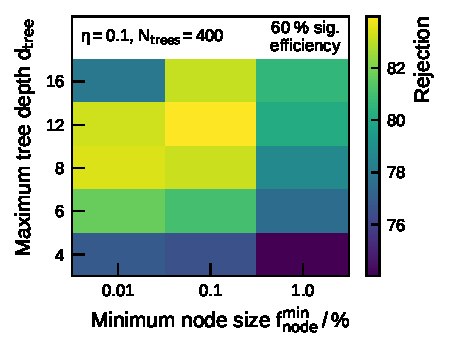
\includegraphics{./figures/bdt_perf/gridsearch_1p/scan_MinNodeSize_MaxDepth.pdf}
    \subcaption{Blablablabla}
  \end{subfigure}
  \caption{Rejection as a function of the hyperparameters. Uses
    \SI{50}{\percent} subsampling.}
  \label{fig:hyperparameter_scan}
\end{figure}

Description of what is seen in the scan:
\begin{itemize}
\item Strong dependence of $N_\text{trees}$ and $d_\text{tree}$: low number
  shallow trees leads to underfitting; high number of deep trees starts to
  degrade performance due to overfitting
\item Strong dependence of shrinkage and number of trees: Very narrow maximum in
  feature space - shrinkage has to be tuned for the number of trees. Significant
  overfitting in high shrinkage high ntree region.
\item Maximum tree depth vs shrinkage: Deep trees need low shrinkage to avoid
  overfitting and vice versa for underfitting.
\item Maximum tree depth vs minnodesize: Critical parameter to set correctly. If
  set too large severe underfitting is observed. For small minimum node sizes
  one has to be careful to not set the tree depth too high since minimum node
  size is the depth limiter in most cases. One tuning strategy could be to set
  the tree depth to very large values and just limit using minimum node size but
  this would require fine tuning for different sample sizes.
\end{itemize}

\begin{figure}[ht]
  \centering
  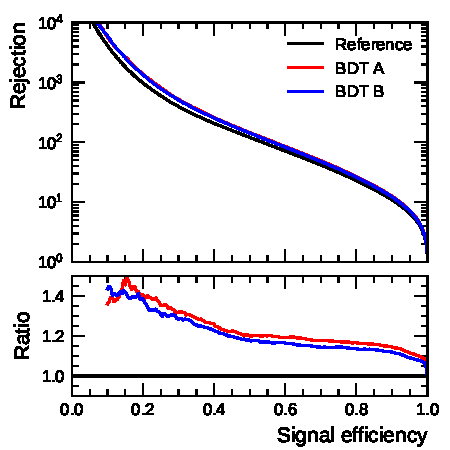
\includegraphics{./figures/bdt_perf/roc/bdt_1p_comparison.pdf}
  \caption{\emph{ROC}-Curve for 1-prong.}
  \label{fig:bdt_1p_roc}
\end{figure}



\subsection{Working Points}
\label{sec:bdt_working_points}

Working points (Gammatautau -- Ztautau)

Signal efficiencies 1P (3P):
\begin{itemize}
\item Very Loose: 95\% (95\%)
\item Loose: 85\% (75\%)
\item Medium: 75\% (60\%)
\item Tight: 60\% (45\%)
\end{itemize}

\section{Feature Selection}
\label{sec:bdt_feature_selection}

\subsection{Variable Importance}
\label{sec:bdt_var_importance}

Variable correlations, importance (dropped variables) \& dependence with
$p_\mathrm{T}$ (2D Hist - including pt), Variable Transformations (instead
of cutting out outliers), Partial Dependence, Including $p_\mathrm{T}$

\section{Identification Performance on Simulated Data}
\label{sec:bdt_perf}

\subsection{Performance in Simulation}
\label{sec:bdt_perf_sim}

Impact on (reconstructed) decay modes (?)

\subsubsection{Performance on Quark- / Gluon-initiated Jets}
\label{sec:bdt_perf_quark_gluon}

Impact of Quark / Gluon initiated jets on Tau-ID (i.e. performance of ID
on Quark / Gluon jets)

\subsection{Performance on Data}
\label{sec:bdt_perf_data}

Performance on TAUP4 (?)

% -------------------------------------------------------------------------- %
\begin{itemize}
\item Description \& Plots of the input variables
  \begin{itemize}
  \item How does etOverPtLeadTrk differ from EMPOverTrkSysP for 1-prong taus?
  \end{itemize}

\item Preselection
  \begin{itemize}
  \item $p_\mathrm{T} > \SI{20}{\GeV}$ (reconstructed \& truth)
  \item $| \eta | < 2.5$ (reconstructed \& truth)
  \item $| \eta | \notin \left[ 1.37, 1.52 \right]$ (reconstructed \& truth)
  \item truth-matched taus
  \end{itemize}

\item Train baseline for comparison (with default outlier removal)
  \begin{itemize}
  \item NTrees 100 (explain)
  \item MinNodeSize 0.1 (explain)
  \item BoostType AdaBoost (explain)
  \item SeparationType GiniIndex (explain)
  \item PruneMethod NoPruning
  \item UseYesNoLeaf False (explain)
  \item AdaBoostBeta 0.2 (explain)
  \item DoBoostMonitor True
  \item nCuts 200 (explain)
  \item MaxDepth 8 (explain)
  \end{itemize}

\item Switch from AdaBoost to GradBoost (Explain why we don't do a full
  optimization of the AdaBoost vs GradBoost setup)

\item Variable transformations (log, clamp, uniformization)
  \begin{align}
    &\text{SumPtTrkFrac:} &\log(x + 10^{-4}) \\
    &\text{absipSigLeadTrk:} &\min(x, 30) \\
    &\text{mEflowApprox:} &\log(x) \\
    &\text{centFrac:} &\min(x, 1) \\
    &\text{innerTrkAvgDist:} &- \\
    &\text{ptRatioEflowApprox:} &\min(x, 4) \\
    &\text{EMPOverTrkSysP:} &\log(\max(10^{-3}, x)) \\
    &\text{etOverPtLeadTrk:} &\log(\max(0.1, x)) \\
    &\text{ChPiEMEOverCaloEME:} &\max(-4, \min(x, 5)) \\
    &\text{trFlightPathSig:} &\log(\max(0.01, x)) \\
    &\text{massTrkSys:} &\log(x) \\
    &\text{dRmax:} &-
  \end{align}

\item Variable importance (Google: Variable Importance Measures)
  \begin{itemize}
  \item Drop-one test
  \item Partial dependence (can we use a two way partial dependence plot to
    show interaction of pt and another variable?)
    \url{http://scikit-learn.org/stable/modules/ensemble.html#interpretation}
  \end{itemize}

\item $p_\mathrm{T}$-dependency 2D histograms of (centFrac / innerTrkAvgDist --
  worse \& SumPtTrkFrac -- should get better) (Plot 'variable separation' vs.
  pt)

\item Performance on gluon / quark initiated jets

\item Cross check with data (jets only)?

\end{itemize}

%%% Local Variables:
%%% mode: latex
%%% TeX-master: "mythesis"
%%% End:

\chapter{RNN}
\label{sec:rnn}

\begin{itemize}
\item Track-RNN
  \begin{itemize}
  \item Replace $\Delta R_\mathrm{JS}$ with $\Delta \eta$ and $\Delta \varphi$
    (try extrapolated \& non-extrapolated)
  \item Replace pt asymmetry with $pt_\mathrm{JS}$
  \item Do a validation loss vs.\ number of tracks scan
  \item Validation loss vs.\ sample size
  \end{itemize}

\item Cluster-RNN
  \begin{itemize}
  \item
  \end{itemize}

\item Combined-RNN
  \begin{itemize}
  \item
  \end{itemize}
\end{itemize}


%%% Local Variables:
%%% mode: latex
%%% TeX-master: "mythesis"
%%% End:

% ~ 8-10 pages
\chapter{Decay Mode Classification of Hadronically Decaying $\tau$-Leptons}
\label{sec:decaymode}

In this chapter the sequence learning techniques developed for
tau-identification are applied to the problem of decay mode classification of
hadronic tau lepton decays. In the following the decay modes containing one
charged hadron $h^\pm$ with one $h^\pm \pi^0$ or more than one neutral pion
$h^\pm \geq 2\pi^0$ as well as three charged hadrons without neutrals $3h^\pm$
or at least one neutral pion $3h^\pm \geq 1\pi^0$ shall be discriminated. The
hadron $h^\pm$ includes charged pions as well as kaons while decays over
intermediate $\text{K}^0$ are omitted. These five decay modes make up the
majority of hadronic tau lepton decays (approx. \SI{92}{\percent}). Neural
networks naturally extend from binary to multi-class classification problems
making them well-suited for the discrimination of the hadronic decay modes.

At first a quick overview of the \emph{Tau Particle Flow}-algorithm is given,
which is used to reconstruct neutral and charged decay products. Subsequently a
neural network is developed that uses the reconstructed decay products to
classify the decay mode into one of five categories. Finally the network is
extended by including additional information from conversion tracks, cluster
moments and shot information. In the following the notation established in
\cite{atlas:taurec:decaymodes} will be adopted.

\todo[inline]{Signature of the decay modes (Could be moved to
  \textit{Theoretical Background})}

\section{Tau Particle Flow}
\label{sec:tau_pflow}

The \emph{Tau Particle Flow}-algorithm is a specialised particle flow algorithm
for reconstruction of charged and neutral constituents in hadronic tau decays
with visible transverse momenta of up to \SI{100}{\giga\electronvolt}. It aims
to improve reconstruction of individual particles by optimally combining the
information in several subdetector-systems. The reconstructed objects, called
charged or neutral \emph{particle flow objects}~(PFOs), can be used to classify
the hadronic decay modes and for improving the energy resolution of the
reconstructed hadronic tau decay by employing a decay mode specific calibration.
The following description of the algorithm is based on
\cite{atlas:taurec:decaymodes} including recent changes to the reconstruction
algorithms.

Charged PFOs are reconstructed from tracks classified as \emph{charged}
according to the track classification. The charge and transverse momentum of the
reconstructed PFO is determined from the measurement in the tracking system,
which has superior energy resolution for charged pions with
$p_\text{T} < \SI{100}{\giga\electronvolt}$ compared to a calorimeter-based
measurement~\cite{atlas:taurec:decaymodes}. The $\pi^\pm$-mass hypothesis is
used to calculate the energy of the PFO. Charged hadrons initiate extensive
hadronic showers depositing most of their energy in the hadronic calorimeters
(incl.\ EM3) \todo{Motivation for this sentence?}.

Neutral pions often deposit their energy in a single cluster in the EM
calorimeter (Presampler, EM1/EM2) caused by two collimated photons from the
$\pi^0$ decay. Therefore neutral PFOs are reconstructed by clustering all cells
in the electromagnetic part of the calorimeter within the $\Delta R < 0.4$ cone
about the tau axis \todo{Check instead of core-region?}. If a cluster is in the
proximity of a charged PFO then the energy deposition of the charged hadron in
the EM calorimeter has to be separated from the neutral pion energy. The energy
$E_{h^\pm}^{\text{EM}}$ that needs to be subtracted to remove the contribution
of the charged hadron is estimated by
\begin{align*}
  E_{h^\pm}^{\text{EM}} = E_{h^\pm}^{\text{track}} - E_{h^\pm}^{\text{HAD}} \eqcomma
\end{align*}
where $E_{h^\pm}^{\text{track}}$ is the energy of the charged PFO measured in
the tracking system and $E_{h^\pm}^{\text{HAD}}$ the energy of the charged PFO
deposited in the hadronic part of the calorimeter. $E_{h^\pm}^{\text{HAD}}$ is
calculated by matching clustered energy deposits in the HCAL to the closest
track of a charged PFO. The contribution of the charged hadron in the EM
calorimeter~$E_{h^\pm}^{\text{EM}}$ is subtracted from the closest neutral PFO
cluster if the angular distance between cluster and extrapolated track is
smaller than $\Delta R < 0.04$. \todo{Zero mass hypothesis for neutrals?}
Neutral PFOs can often be reconstructed from an incomplete subtraction of the
charged hadron energy deposition in the EM calorimeter or by pile-up. For decay
mode classification it is necessary to identify the neutral pions in all
reconstructed neutral PFOs of the tau decay. The identification exploits the
difference in shower shape of hadronic showers initiated by charged hadrons and
compact showers from photons of the $\pi^0$ decay using multivariate methods.

The number of identified neutral pions can be used for a preliminary
classification of the decay mode. The following sections will be concerned with
combining reconstructed PFOs in neural networks to achieve better classification
power. Decay mode classification employing the \emph{Tau Particle
  Flow}-algorithm is optimised for operation in the low-momentum regime due to
the decreasing momentum resolution in the tracking system as well as the
additional boost of the tau decay products leading to merging of
$\pi^0$-clusters. Therefore this chapter focuses focus on the classification of
hadronic tau lepton decays with visible transverse
momenta~$p_\text{T} < \SI{100}{\giga\electronvolt}$.

\section{General Idea}
\todo{Better name for this part}
\label{sec:pfo_general}

The charged and neutral PFOs reconstructed with the \emph{Tau Particle
  Flow}-algorithm contain information about the daughter particles of the tau
decay and can be used for decay mode classification. Properties of charged and
neutral PFOs are combined in recurrent neural networks to perform multi-class
classification. Mainly kinematic information (e.g.\ transverse momentum, angular
deviation from the tau axis) is used to describe each PFO. Moreover the
$\pi^0$-likeness in form of the neutral pion identification BDT score is
included in the classification to be able to discriminate between neutral PFOs
originating from a $\pi^0$ and remnants of the subtraction.

\begin{figure}[htb]
  \centering
  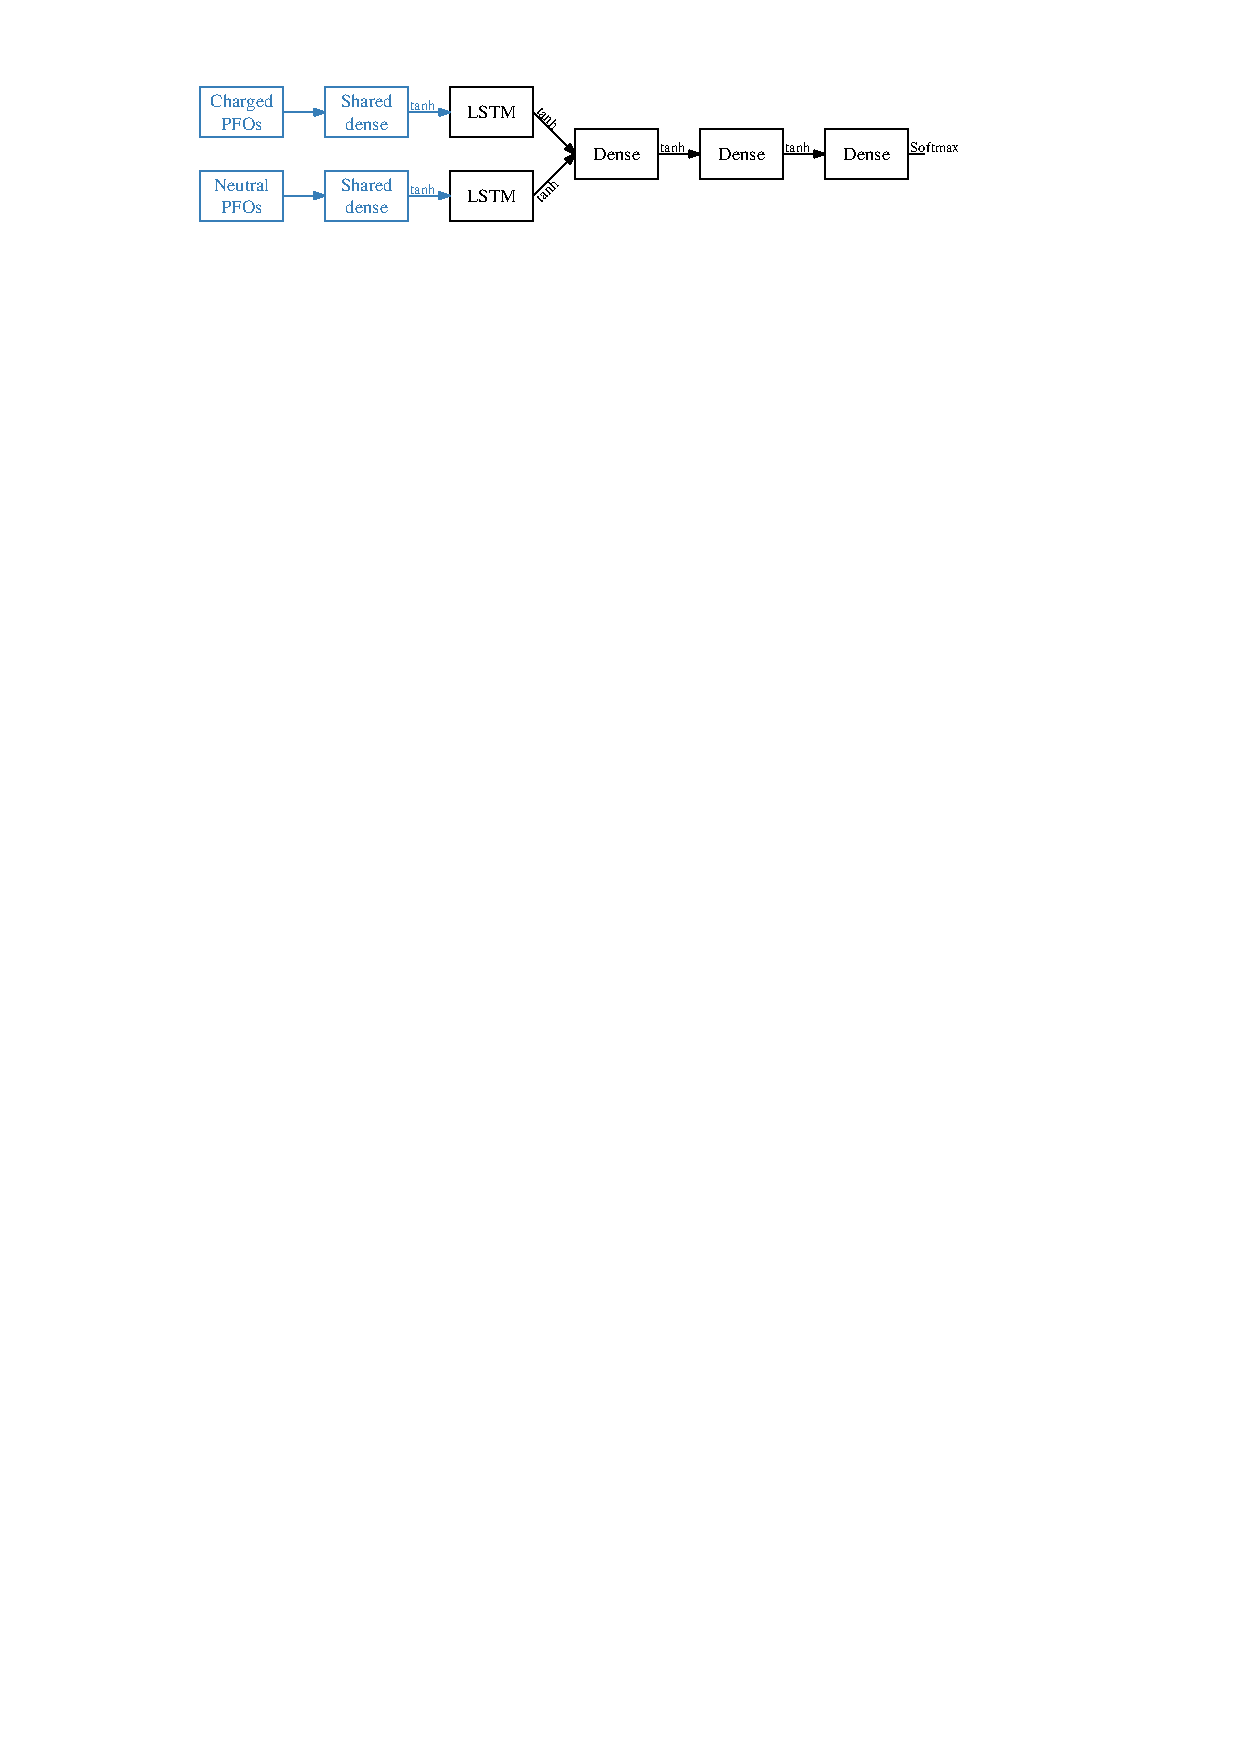
\includegraphics{./figures/decay_mode_classification/baseline_architecture.pdf}
  \caption{Architecture. Highlighted in blue are layers that operate on a sequence of inputs.}
  \label{fig:pfo_rnn_baseline_arch}
\end{figure}

The network architecture used for the decay mode classification is shown in
figure \ref{fig:pfo_rnn_baseline_arch} and is similar to the networks used for
tau-identification in the previous chapter. At the input layer the network is
split into two branches each accepting a number of charged and neutral PFOs
respectively. The shared dense layer\footnote{Applies the same transformation on
  every element of the input sequence} applies an affine transformation on the
input variables of each PFO. Afterwards the input sequences are fed into the
recurrent LSTM layer which subsequently return a single vector of activations.
The activations of both branches are then merged and passed through a network
containing three dense layers. The final dense layer has five units (the number
of decay modes to classify) which are activated by the Softmax activation
function, ensuring that the output activations sum to one.

\todo[inline]{Preselection (same as ID); Low momentum taus:
  $\SI{20}{\giga\electronvolt} < p_\text{T} < \SI{100}{\giga\electronvolt}$;
  Track requirement 1- or 3-prong; Truth decay mode}

\todo[inline]{During the classification the prongness of the decay mode is not
  constrained -- add. migrations are possible}

\section{Baseline}
\label{sec:pfo_baseline}

For training and evaluation of the model a sample containing the process
$\gamma^* \rightarrow \tau \tau \, \text{(hadr.)}$ is used (full sample
identifier in appendix~\ref{sec:app_mc16a_taus}). The baseline tau selection
given in section~\ref{sec:bdt_eventsim} is applied and the visible transverse
momentum~$p_\text{T}$ of the hadronic decay is required to be less than
\SI{100}{\giga\electronvolt} at reconstruction and generator-level. Moreover
only tau-leptons with the true decay mode being one of $h^\pm$, $h^\pm \pi^0$,
$h^\pm \geq 2\pi^0$, $3h^\pm$ or $3h^\pm \geq 1\pi^0$ and omitting decay chains
containing intermediate $\text{K}^0$.

The discrimination of the decay modes utilises kinematic quantities of the
reconstructed tau decay as well as the charged and neutral particle flow
objects:
\begin{description}
\item[Kinematic quantities of the tau decay:] The visible transverse momentum
  $p_\text{T}^\tau$ and the direction $(\varphi_\tau, \eta_\tau)$ of the
  reconstructed tau-axis. The momentum is calibrated at LC-scale
  without applying a tau-specific energy calibration.

\item[Kinematic quantities of charged and neutral PFOs:] The reconstructed
  transverse momentum $p_\text{T}^\text{PFO}$ and the signed angular distances
  to the reconstructed tau decay in transverse\footnote{The definition is
    analogous to the longitudinal case but also accounting for the periodicity
    in $\varphi$.}~$\Delta\varphi$ and longitudinal
  direction~$\Delta\eta \coloneqq \eta_\text{PFO} - \eta_\tau$. The PFO
  directions are given relative to the tau-axis to ensure that coordinates are
  comparable for different tau candidates.
\end{description}
Furthermore the variable set used for the neutral PFOs is extended using:
\begin{description}
\item[$\pi^0$ identification score $S_\text{BDT}^{\pi^0}$:] BDT-based
  discriminant combining cluster information in the electromagnetic part of the
  calorimeter to identify neutral PFOs originating from the $\pi^0$ decay.

\item[Number of shots $N_\text{shots}$:] Number of shots (cmp.\
  section~\ref{sec:shot_reco}) associated with a neutral PFO cluster. Shots are
  associated with a cluster if it contains the seed cell of the shot and the
  cluster fulfils $E_\text{T} > \SI{500}{\mega\electronvolt}$ and is within
  $\Delta R < 0.4$ to the tau axis. In cases where the cell is shared between
  multiple clusters, it is associated to the cluster to which the seed cell
  contributes with the largest weight.

  The fine segmentation of the strip layer of the EM calorimeter is used to
  count local energy maxima created by individual photons and allow to recover
  the correct number of neutrals in cases where the energy depositions of two
  neutral pions are reconstructed as a single cluster in the calorimeter.
\end{description}
\todo[inline]{Give reasons for this variable selection. \SI{1.5}{\percent}}

\todo[inline]{Preprocessing:} The transverse momenta of the reconstructed tau as
well as the PFOs are log-transformed and subsequently standardised (by
subtracting the mean and dividing by the standard deviation of the transformed
variable). The remaining kinematic variables are transformed to fall into the
the $[-1, 1]$ range. For the neutral PFO specific variables
$S_\text{BDT}^{\pi^0}$ and $N_\text{shots}$ no preprocessing is needed.

Charged and neutral PFOs are passed in ascending transverse momentum ordering to
the shared dense layers with 24 units each. The intermediate representation of
the input sequence is then passed into the LSTM layers each with 24 units and
hard sigmoid recurrent activation. The recurrent layers return a single element
containing 24 scalar values which are subsequently merged and passed through
three dense layers with 48, 32 and 5 units respectively. The outputs of the
different layers are activated using the $\tanh$ activation function with the
exception of the last dense layer, which uses \emph{Softmax} activation.

For each reconstructed tau decay the model returns one probability for each of
the five decay modes. The reconstructed decay mode is then given as the mode
with the highest probability according to the model. A different scheme for
determining the decay mode would be to require the largest mode probability to
exceed the second largest by a predefined margin. This would increase the purity
of the reconstructed modes at the expense of reducing the reconstruction
efficiency (should be evaluated on analysis-level).

In contrast to the decay mode classification algorithm currently in use at the
ATLAS experiment, no discrimination of 1- and 3-prong modes according to the
number of tracks that are classified as \emph{charged} is made. However each
charged PFO is associated with a \emph{charged} track such that the number of
tracks is indirectly available to the network. The network is not strictly
required to use this information allowing migrations of reconstructed 1-track
(3-track) hadronic tau decays to 3-prong (1-prong) modes. If this behaviour is
not desired then the decay mode can be classified as the mode with the highest
probability that is still compatible with the number of reconstructed tracks.

Reconstructed hadronic tau decays contain neutral PFOs that are not originating
from neutral pions but from other sources. Moreover it is not known how well
these PFOs are modelled in the simulation that is used to train and evaluate the
models. Therefore the neutral PFOs used in the RNN are required to pass a
$p_\text{T}$-threshold. Table \ref{tab:neut_ptcut} summarises the diagonal
efficiency of the classification for four different thresholds \todo{Requires
  retraining of the model!}.
\begin{table}[htb]
  \centering
  \begin{tabular}{SS[table-format=2.2(2)]}%,table-space-text-post = \si{\meter}]}
  \toprule
  {$p_\text{T}$-cut / \si{\giga\electronvolt}} & {Diagonal efficiency / \si{\percent}} \\
  \midrule
  {--} & 78.43 \pm 0.06 \\
  1.0 & 78.09 \pm 0.08 \\
  1.5 & 77.95 \pm 0.04 \\
  2.0 & 77.88 \pm 0.06 \\
  2.5 & 77.54 \pm 0.04 \\
  \bottomrule
\end{tabular}

%%% Local Variables:
%%% mode: latex
%%% TeX-master: "../mythesis"
%%% End:

  \caption{Impact of a neutral $p_\text{T}$-cut on the diagonal
    efficiency.}
  \todo[inline]{Motivate \SI{1.5}{\giga\electronvolt} cut.}
  \label{tab:neut_ptcut}
\end{table}
It is observed that the overall classification performance does not degrade when
no $p_\text{T}$-cut is applied, indicating that the network is able to (since
$p_\text{T}^\text{PFO}$ is an input). Moreover the accuracy does not decrease
drastically \todo{better word?} when the threshold is increased such that a
threshold can be applied if it turns out that low momentum PFOs show significant
mismodelling. For further studies the \SI{1.5}{\giga\electronvolt} threshold is
used.

\todo[inline]{Explain migration and composition matrices. Explain that the
  trainings are not 'stable' in the sense that classification power can be
  redistributed across different modes i.e.\ a decrease in one mode can be
  compensated by improvements in another.}

\begin{figure}[htb]
  \begin{subfigure}[t]{0.48\textwidth}
    \centering
    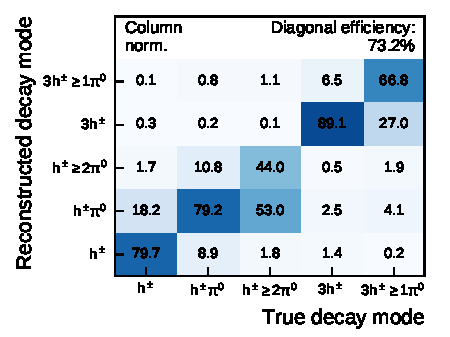
\includegraphics{./figures/decay_mode_classification/mig_mat_pantau.pdf}
    \subcaption{ATLAS default algorithm: \emph{PanTau}}
  \end{subfigure}\hfill
  \begin{subfigure}[t]{0.48\textwidth}
    \centering
    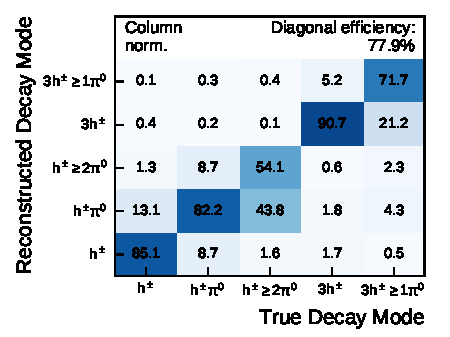
\includegraphics{./figures/decay_mode_classification/mig_mat_baseline_ptcut_1_5.pdf}
    \subcaption{PFO-RNN with neutral $p_{\text{T}}$-cut of
      \SI{1.5}{\giga\electronvolt}}
  \end{subfigure}
  \caption{Migration matrices with normalised columns showing the migration of
    the true decay modes to the reconstructed modes. }
  \todo[inline]{After reconstruction in
    $\gamma^* \rightarrow \tau \tau \, \text{hadr.}$ and omitting decays
    containing neutral kaons.}
  \label{fig:migmat}
\end{figure}


\begin{figure}[htb]
  \begin{subfigure}[t]{0.48\textwidth}
    \centering
    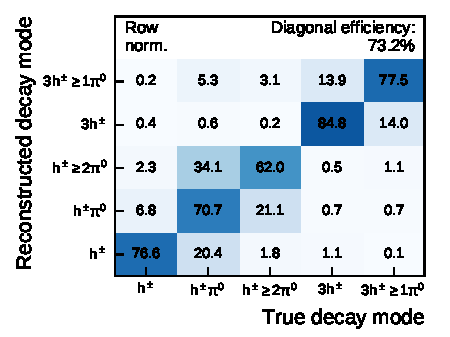
\includegraphics{./figures/decay_mode_classification/comp_mat_pantau.pdf}
    \subcaption{ATLAS default algorithm: \emph{PanTau}}
  \end{subfigure}\hfill
  \begin{subfigure}[t]{0.48\textwidth}
    \centering
    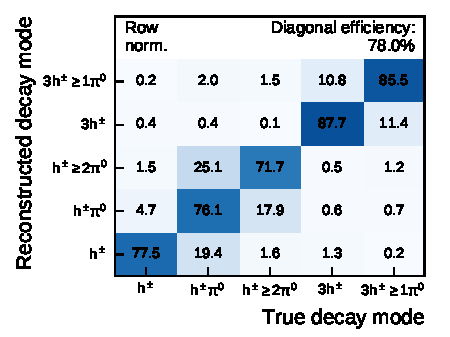
\includegraphics{./figures/decay_mode_classification/comp_mat_baseline_ptcut_1_5.pdf}
    \subcaption{PFO-RNN with neutral $p_{\text{T}}$-cut of
      \SI{1.5}{\giga\electronvolt}}
  \end{subfigure}
  \caption{Composition matrices with normalised rows showing the migration of
    the true decay modes to the reconstructed modes.}
  \label{fig:migmat}
  \todo[inline]{Check whether the 'diagonal efficiency' is correct for
    composition matrices.}
\end{figure}


\begin{figure}[ht]
  \begin{subfigure}[t]{0.48\textwidth}
    \centering
    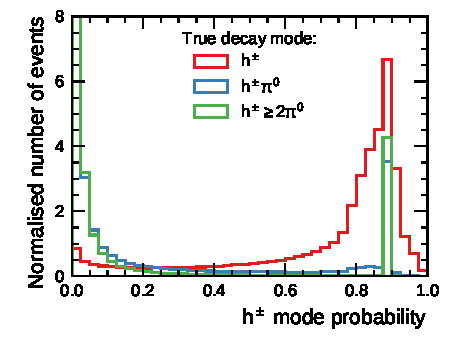
\includegraphics{./figures/decay_mode_classification/mode_proba_baseline_ptcut_1_5_only_1p/proba_1p0n.pdf}
    \subcaption{In most cases the probabilities for modes containing neutral
      pions to be classified as the $h^\pm$ mode are small. However in cases
      where no neutral PFO is reconstructed the probabilities can be large
      \SI{90}{\percent}.}
  \end{subfigure}\hfill
  \begin{subfigure}[t]{0.48\textwidth}
    \centering
    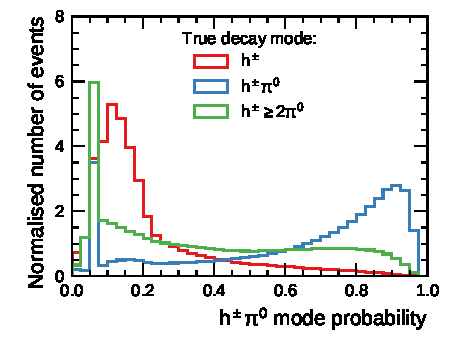
\includegraphics{./figures/decay_mode_classification/mode_proba_baseline_ptcut_1_5_only_1p/proba_1p1n.pdf}
    \subcaption{The discrimination of modes with one neutral and more than one
      neutral pion is difficult. In cases of no reconstructed neutral pions the
      probabilities can be small ($\approx \SI{5}{\percent}$)}
  \end{subfigure}
  \caption{Mode probabilities for the $h^\pm$ and $h^\pm \pi^0$ modes. While
    each tau candidate is assigned a probability for all five decay modes the
    probabilities for the 3-prong modes have been omitted.}
  \label{fig:mode_proba_ptcut}
\end{figure}

\section{Additional Information}

\begin{description}
\item[Conversion tracks] Often photons from the $\pi^0$ decay convert into
  electron-positron pairs in the material of the inner detector. Conversions can
  therefore \todo{Why? Electrons bent out of cone? Neutral PFOs fail $\pi^0$-ID?
    Will the electrons be reconstructed in neutral PFOs?} lead to an
  underestimation of the number of neutral pions. The inclusion of conversion
  tracks in the classification aims to reduce migrations to decay modes with
  fewer neutrals.

\item[Shots] Due to the boosted topology of tau decays in ATLAS (especially at
  high-$p_\text{T}$) neutral pion clusters can merge with the charged or another
  neutral pion leading to a reduction in the reconstructed number of neutrals.
  Information on nearby shots \todo{NHitsInEM1 is already in the neut.\ PFOs}
  can further improve classification.

\item[Add. cluster moments] Further improvements in classifying merged clusters
  can be achieved by using shower shape information similar to what is used for
  the $\pi^0$ identification.
\end{description}

\begin{description}
\item[Width $\langle R^2 \rangle$]
\item[$\eta$ width in EM1 $\langle (\eta - \eta_\text{cluster})^2\rangle$]
\item[Number of positive cells in EM1 $N_\text{EM1}^\text{pos}$]
\item[Core energy fraction $f_\text{core}$] Fraction of the total cluster energy
  contained in the highest energy cells of Presampler, EM1 and EM2.
\item[Energy fraction in EM2 $f_\text{EM2}$] Fraction of total cluster energy in
  EM2.
\end{description}
Longitudinal moments were not found to lead to an increase performance.


Neutral PFOs (Charged PFOs + whats listed here):
\begin{itemize}
\item $f_\text{core}$: Fraction of energy contained in the  calorimeter cells



  \texttt{ENG\_FRAC\_CORE} Fraction of energy in the three
  hottest cells in each sampling \todo{Check}
\item $f_\text{EM2} = E_\text{EM2} / E$: Energy fraction in EM2 \todo{Why not
    EM1? -- Energy fraction is highly anti-correlated with EM1 therefore only
    one is chosen.}
\end{itemize}

\begin{table}[htb]
  \centering
  \begin{tabular}{p{5cm}S[table-format=1.4(4)]S[table-format=2.2(2)]S[table-format=1.2(2)]}
  \toprule
  {Experiment} & {Loss} & {Diag.\ eff.\ / \si{\percent}} & {Diag.\ eff.\ gain (abs.) / \si{\percent}} \\
  \midrule
  Conversion tracks & 0.5186 +- 0.0013 & 79.40 +- 0.07 & 1.45 +- 0.08 \\
  Conversion tracks (extrapol.) & 0.5224 +- 0.0012 & 79.23 +- 0.06 & 1.28 +- 0.07 \\
  Shots & 0.5239 +- 0.0011 & 79.52 +- 0.06 &  1.57 +- 0.07 \\
  Neut.\ PFO cluster properties & 0.5310 +- 0.0010 & 79.07 +- 0.06 & 1.12 +- 0.07 \\
  Hadronic PFOs & 0.5433 +- 0.0007 & 78.30 +- 0.04 & 0.35 +- 0.06 \\
  Fraction of subtracted $p_\text{T}$ & 0.5466 +- 0.0005 & 78.26 +- 0.03 & 0.31 +- 0.05 \\
  $\pi^0$-BDT ordering & 0.5511 +- 0.0013 & 78.01 +- 0.07 & 0.06 +-0.08 \\
  \bottomrule
\end{tabular}

%%% Local Variables:
%%% mode: latex
%%% TeX-master: "../mythesis"
%%% End:

  \caption{Additional experiments}
  \label{tab:pfo_add_experiments}
\end{table}

\begin{align*}
  f_\text{sub} = \frac{p_{\text{T}}^{\text{cluster}} - p_{\text{T}}^{\text{PFO}}}{p_{\text{T}}^{\text{PFO}}}
\end{align*}

\todo[inline]{Try out bidirectional LSTMs and stacked ones (still not
  overfitting).Technically would allow multiple outputs: Could do Pi0 Cluster-ID
  internally. What else has been tested?}

\section{Combining Everything}

\begin{figure}[!ht]
  \begin{subfigure}{0.48\textwidth}
    \centering
    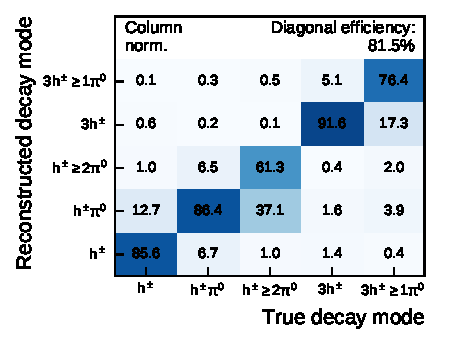
\includegraphics{./figures/decay_mode_classification/combined_sub_e_moments_shots_conv_ptcut_1_5/mig_mat.pdf}
    \subcaption{Migration matrix}
  \end{subfigure}\hfill
  \begin{subfigure}{0.48\textwidth}
    \centering
    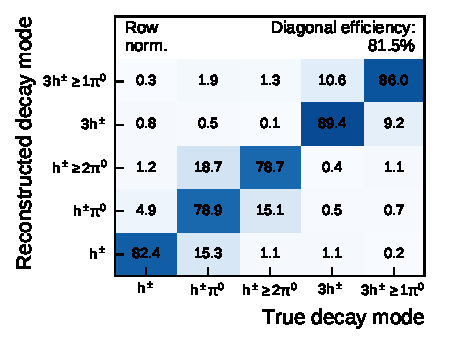
\includegraphics{./figures/decay_mode_classification/combined_sub_e_moments_shots_conv_ptcut_1_5/comp_mat.pdf}
    \subcaption{Composition matrix}
  \end{subfigure}
  \caption{Combined}
  \label{fig:decay_mode_combined}
\end{figure}

\begin{figure}[!ht]
  \begin{subfigure}{0.48\textwidth}
    \centering
    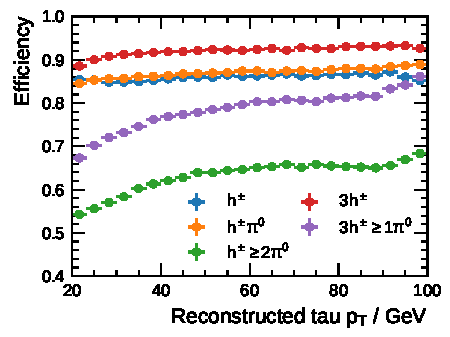
\includegraphics{./figures/decay_mode_classification/combined_sub_e_moments_shots_conv_ptcut_1_5/efficiency_profile.pdf}
    \subcaption{Efficiency profile}
  \end{subfigure}\hfill
  \begin{subfigure}{0.48\textwidth}
    \centering
    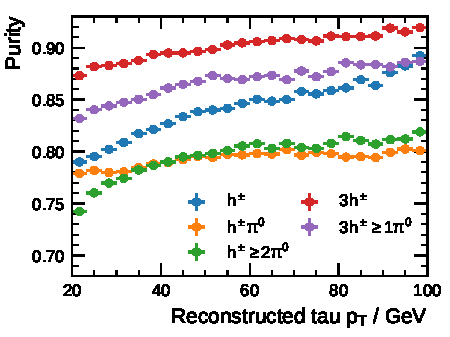
\includegraphics{./figures/decay_mode_classification/combined_sub_e_moments_shots_conv_ptcut_1_5/purity_profile.pdf}
    \subcaption{Purity profile}
  \end{subfigure}
  \caption{$p_\text{T}$-dependence of mode efficiency and purity}
  \label{fig:mode_efficiency_purity}
\end{figure}

\todo[inline]{Class probabilities (showing the non-existent peak). Improvements
  for Higgs CP measurement in
  $H \rightarrow \tau\tau \rightarrow \rho \rho 2\nu$. Performance when applying
  medium tau identification. Fluid classification -- a single PFO is not
  'causing' a particular classification result -- could use heuristic methods to
  reconstruct neutral pions after classification. Unleash on data without upper
  $p_\text{T}$ limit.}

\begin{table}[htb]
  \centering
  \begin{tabular}{
  l
  S[table-format=2.2(2)]
  S[table-format=2.1(2)]
  S[table-format=2.1, round-mode=places, round-precision=1]
  S[table-format=2.1, round-mode=places, round-precision=1]
  }
  \toprule
  {Mode} & {$\mathcal{B}$ / \si{\percent}} & {$f_\text{BR}$ / \si{\percent}} & {$f_\text{reco}$ / \si{\percent}} & { $f_\text{reco+ID}$ / \si{\percent}} \\
  \midrule
  $h^\pm$ & 11.51 +- 0.05 & 18.3 +- 0.1 & 17.552988 & 21.365416 \\
  $h^\pm \pi^0$ & 25.93 +- 0.09 & 41.3 +- 0.2 & 41.854581 & 44.779216 \\
  $h^\pm \geq 2 \pi^0$ & 10.81 +- 0.09 & 17.2 +- 0.2 & 18.663134 & 15.775690 \\
  $3 h^\pm$ & 9.43 +- 0.05 & 15.1 +- 0.1 & 14.200414 & 13.315444 \\
  $3 h^\pm \geq 1 \pi^0$ & 5.09 +- 0.05 & 8.1 +- 0.1 & 7.728881 & 4.764232 \\
  \bottomrule
\end{tabular}

%%% Local Variables:
%%% mode: latex
%%% TeX-master: "../mythesis"
%%% End:

  \caption{Mode reconstruction efficiencies. $h^\pm$ can be pion or kaon.
    Intermediate decays via neutral kaons are excluded. Branching fraction
    $\mathcal{B}$; Mode fractions of reconstructed taus passing preselection
    $f_\text{reco}$; Mode fraction of taus also passing medium tau id.}
  \todo[inline]{Do the fractions make sense? Make comparable to branching
    ratio?}
  \label{tab:mode_reco_eff}
\end{table}

\begin{figure}[!ht]
  \begin{subfigure}{0.48\textwidth}
    \centering
    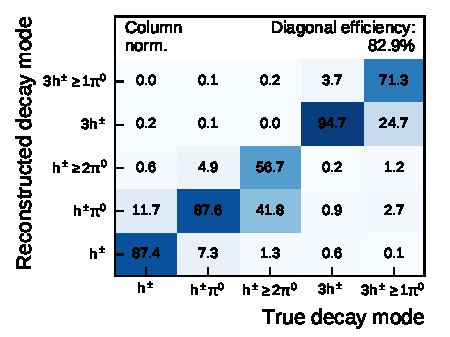
\includegraphics{./figures/decay_mode_classification/combined_sub_e_moments_shots_conv_ptcut_1_5/mig_mat_med_id.pdf}
    \subcaption{Migration matrix}
  \end{subfigure}\hfill
  \begin{subfigure}{0.48\textwidth}
    \centering
    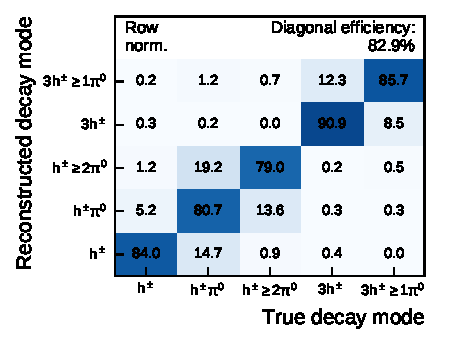
\includegraphics{./figures/decay_mode_classification/combined_sub_e_moments_shots_conv_ptcut_1_5/comp_mat_med_id.pdf}
    \subcaption{Composition matrix}
  \end{subfigure}
  \caption{Combined with medium tau id}
  \label{fig:decay_mode_combined_med_id}
\end{figure}

\clearpage
\subsection{High-$p_\text{T}$ performance}
\begin{figure}[htb]
  \begin{subfigure}{0.48\textwidth}
    \centering
    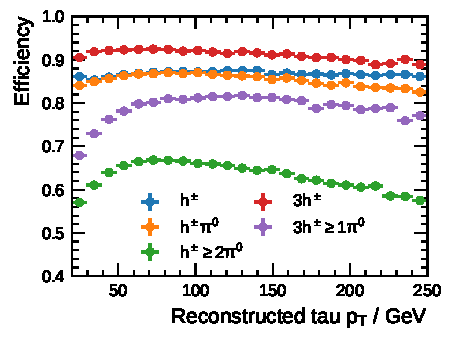
\includegraphics{./figures/decay_mode_classification/highpt/efficiency_profile.pdf}
    \subcaption{Efficiency profile}
  \end{subfigure}\hfill
  \begin{subfigure}{0.48\textwidth}
    \centering
    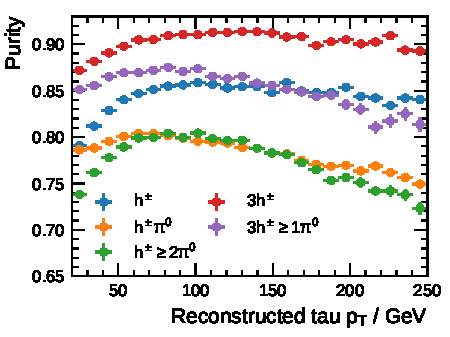
\includegraphics{./figures/decay_mode_classification/highpt/purity_profile.pdf}
    \subcaption{Purity profile}
  \end{subfigure}
  \caption{$p_\text{T}$-dependence of mode efficiency and purity}
  \label{fig:mode_efficiency_purity_highpt}
\end{figure}

\begin{figure}[htb]
  \begin{subfigure}{0.48\textwidth}
    \centering
    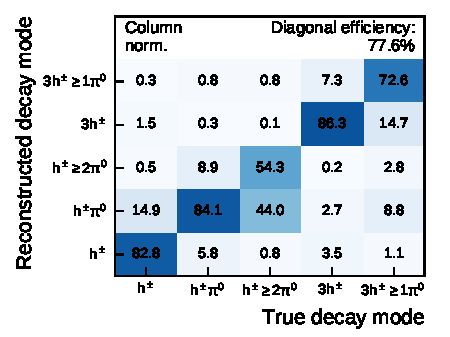
\includegraphics{./figures/decay_mode_classification/highpt/mig_mat_pt_geq_100.pdf}
    \subcaption{Migration matrix. $p_\text{T} > \SI{100}{\giga\electronvolt}$}
  \end{subfigure}\hfill
  \begin{subfigure}{0.48\textwidth}
    \centering
    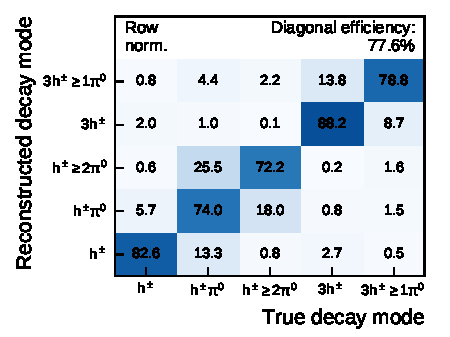
\includegraphics{./figures/decay_mode_classification/highpt/comp_mat_geq_100.pdf}
    \subcaption{Composition matrix. $p_\text{T} > \SI{100}{\giga\electronvolt}$}
  \end{subfigure}
  \caption{highpt}
  \label{fig:highpt_matrices}
\end{figure}


%%% Local Variables:
%%% mode: latex
%%% TeX-master: "mythesis"
%%% End:

% ~ 1-2 pages
\chapter{Summary and Outlook}
\label{sec:conclusion}

The performance of the reconstruction and identification algorithms for hadronic
tau lepton decays are of large importance in the ATLAS experiment. They form the
foundation for many physics analyses involving tau leptons. As a result,
improving the performance of these algorithms can lead to significant benefits
for numerous analyses.

In this thesis the tau identification algorithm currently employed in the ATLAS
experiment is optimised. The configuration of the BDT used for identification is
systematically optimised and the variable selection revised. The background
rejection is improved by \num{10} to \SI{30}{\percent} for \tauhadvis \pt below
\SI{200}{\GeV} at the fixed signal efficiency working points. For fake
\tauhadvis candidates with \pt above \SI{200}{\GeV} the rejection is improved by
up to \SI{80}{\percent}.
% No increase in inherent complexity?

A method of performing tau identification based on neural networks is presented.
For this the BDT-based identification is reproduced using a simple neural
network. Subsequently, a novel approach employing sequence learning techniques
to discriminate hadronic tau lepton decays from quark- and gluon-initiated jets
is presented. Sequences of charged-particle tracks associated with a \tauhadvis
candidate are combined in a recurrent neural network to reject fake \tauhadvis
candidates. The model presented in this thesis shows performance characteristics
similar to the optimised BDT-based identification using high-level variables,
while almost exclusively using tracking information. The background rejection of
this model exceeds (misses) the rejection of the optimised 1-prong (3-prong)
identification by \num{10} to \SI{20}{\percent}, indicating that the current
algorithm does not fully exploit the isolation information in the track system.

Similarly, the approach is applied to reconstructed clusters of energy in the
calorimeter system. The rejection of a purely cluster-based identification is
insufficient for offline tau identification. A study is presented showing the
benefits of using TopoClusters in the \emph{Global Trigger System} of the HL-LHC
to reduce the trigger rates of a ditau trigger. The target rate of
\SI{200}{\kilo\hertz} could be achieved with \tauhadvis \pt thresholds of
\SI{25}{\GeV} and ditau efficiencies of approximately \SI{90}{\percent} on the
plateau starting at true \tauhadvis \pt of \SI{40}{\GeV}.

The tau identification studies are concluded with a model combining track,
cluster and high-level variables. The model shows a significant increase in
rejection of approximately \SI{50}{\percent} for fake \tauhadvis candidates at
low \pt. The improvement in background rejection exceeds a factor of two
starting at \tauhadvis \pt of \SI{60}{\GeV} (\SI{100}{\GeV}) for the 1-prong
(3-prong) identification. Analyses with large backgrounds from quark- or
gluon-initiated jets could directly benefit from the improved background
rejection. In cases where the rejection of the current identification is
sufficient, an identification working point with higher signal efficiency can be
employed. In an exemplary analysis measuring a ditau resonance that requires two
tight \tauhadvis, the signal yield of the $\tauhad\tauhad$ channel could be
increased by approximately \SI{30}{\percent}.

Finally, the sequence learning techniques developed in this thesis are applied
to the problem of decay mode classification of hadronic tau decays. For this
constituents of the decay reconstructed with the \emph{Tau Particle Flow}
algorithm are combined in a recurrent neural network to classify the decay mode.
The network is well-suited to perform multiclass classification showing an
improvement in classification accuracy from \num{73.2} to \SI{78.0}{\percent},
thus reducing the number of misclassified decays by almost \SI{20}{\percent}.
The model is extended by including conversion track, shot and neutral PFO
cluster information further improving the accuracy to \SI{81.0}{\percent} and
reducing the misclassifications by approximately \SI{30}{\percent}. The
improvement in classification accuracy could improve the energy calibrations
used for hadronic tau decays, leading to more accurate mass reconstruction of
tau resonances improving the signal extraction process in analyses. For future
measurements of the \cp nature of the Higgs boson it allows to select hadronic
decay modes more efficiently and with higher purity.

Continued work on the algorithms presented in this thesis is planned. While the
studies on the BDT-based identification are largely implemented in the ATLAS
reconstruction framework, the models based on neural networks still allow for
further optimisations. The network architectures allow for countless variations
that could further improve the performance of the identification. The validation
of the network performance on collision data is still pending. Potential
differences in simulation and data could be resolved by training the tau
identification using background samples collected with dijet triggers, which was
done for the identification in Run 1. The infrastructure necessary to evaluate
the models in the ATLAS reconstruction framework is actively being worked on,
such that the models presented in this thesis could be available to analyses of
Run~2 collision data.

%%% Local Variables:
%%% mode: latex
%%% TeX-master: "mythesis"
%%% End:

% Uncomment the following command to get references per chapter.
% Put it inside the file or change \include to \input if you do not want the references
% on a separate page
% \printbibliography[heading=subbibliography]

%------------------------------------------------------------------------------
% Use biblatex for the bibliography
% Add bibliography to Table of Contents
% Comment out this command if your references are printed for each chapter.
\printbibliography[heading=bibintoc]

%------------------------------------------------------------------------------
% Include the following lines and comment out \printbibliography if
% you use BiBTeX for the bibliography.
% If you use biblatex package the files should be specified in the preamble.
% \KOMAoptions{toc=bibliography}
% {\raggedright
%   \bibliographystyle{../refs/atlasBibStyleWithTitle.bst}
%   % \bibliographystyle{unsrt}
%   \bibliography{./thesis_refs,../refs/standard_refs-bibtex}
% }

%------------------------------------------------------------------------------

\appendix
\addtocontents{toc}{\protect\setcounter{tocdepth}{1}}
% \part*{Appendix}
% Add your appendices here - don't forget to also add them to \includeonly above
%------------------------------------------------------------------------------
\chapter{Auxiliary Information}
\label{sec:app}
%------------------------------------------------------------------------------

\begin{itemize}
\item MC Samples (Preprod, MC16A)
\item BDT ID studies \texttt{bdt\_tauid}
\item RNN ID studies \texttt{rnn\_tauid}
\item RNN Decay Mode studies \texttt{rnn\_decay\_mode\_classif}
\end{itemize}

\todo[inline]{Tables of layers, i.e.\ keras output for model-summary.}

\section{Auxiliary Figures}

\begin{figure}[htpb]
  \centering
  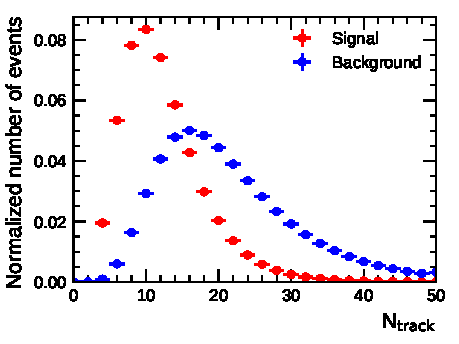
\includegraphics{./figures/rnn/ntrk_3p.pdf}
  \caption{Number of tracks for 3-prong taus}
  \label{fig:total_tracks_3p}
\end{figure}

\begin{figure}[htpb]
  \centering
  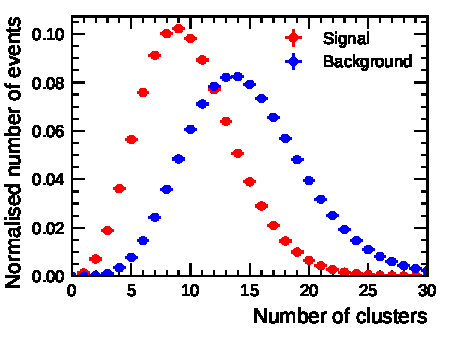
\includegraphics{./figures/rnn/ncls_3p.pdf}
  \caption{Number of clusters for 3-prong taus}
  \label{fig:total_clusters_3p}
\end{figure}

\section{MC Dijet Slices}
Truth $p_\mathrm{T}$ of jet given by anti-$k_\mathrm{T}$ jet algorithm with distance parameter $R=0.6$:
\begin{itemize}
\item[JZ0W] 0 - 20 GeV
\item[JZ1W] 20 - 60 GeV
\item[JZ2W] 60 - 160 GeV
\item[JZ3W] 160 - 400 GeV
\item[JZ4W] 400 - 800 GeV
\item[JZ5W] 800 - 1300 GeV
\item[JZ6W] 1300 - 1800 GeV
\item[JZ7W] 1800 - 2500 GeV
\item[JZ8W] 2500 - 3200 GeV
\end{itemize}

\url{https://svnweb.cern.ch/cern/wsvn/atlasoff/Generators/MC15JobOptions/trunk/share/DSID361xxx/MC15.361021.Pythia8EvtGen_A14NNPDF23LO_jetjet_JZ1W.py}


\url{https://svnweb.cern.ch/cern/wsvn/atlasoff/Generators/MC15JobOptions/trunk/common/Filters/JetFilterAkt6.py}


\url{https://svnweb.cern.ch/cern/wsvn/atlasoff/Generators/MC15JobOptions/trunk/common/Filters/JetFilter_JZX_Fragment.py}

\todo[inline]{Why is JZ0W not used}

\subsection{Preproduction Taus}
\label{app:preprod_taus}

\begin{lstlisting}[basicstyle=\small\ttfamily, breaklines=true]
  mc16_13TeV.425200.Pythia8EvtGen_A14NNPDF23LO_Gammatautau_MassWeight.merge.AOD.e5468_s2997_r9064_r8996
\end{lstlisting}

19974000 events

\subsection{MC16A Taus}
\label{app:mc16a_taus}

\begin{lstlisting}[basicstyle=\small\ttfamily, breaklines=true]
  mc16_13TeV.425200.Pythia8EvtGen_A14NNPDF23LO_Gammatautau_MassWeight.merge.AOD.e5468_s3126_r9364_r9315
\end{lstlisting}

29998000 events

\subsection{Preproduction Dijets}
\label{app:preprod_dijets}
For the tau identification studies the momentum slices (JZ1W to JZ6W) are
combined without cross section weighting as the sizes of the generated slices
are chosen such that high momentum candidates are enhanced. A cross section
reweighting would significantly reduce the weights of high momentum slices with
a large number of simulated events compared to the low momentum slices (JZ1W -
JZ2W) where only a small number of events are simulated.

\begin{lstlisting}[basicstyle=\small\ttfamily, breaklines=true]
  mc16_13TeV.361021.Pythia8EvtGen_A14NNPDF23LO_jetjet_JZ1W.merge.AOD.e3569_s2997_r9064_r8996
  mc16_13TeV.361022.Pythia8EvtGen_A14NNPDF23LO_jetjet_JZ2W.merge.AOD.e3668_s2997_r9064_r9078
  mc16_13TeV.361023.Pythia8EvtGen_A14NNPDF23LO_jetjet_JZ3W.merge.AOD.e3668_s2997_r9064_r8996
  mc16_13TeV.361024.Pythia8EvtGen_A14NNPDF23LO_jetjet_JZ4W.merge.AOD.e3668_s2997_r9064_r9078
  mc16_13TeV.361025.Pythia8EvtGen_A14NNPDF23LO_jetjet_JZ5W.merge.AOD.e3668_s2997_r9064_r8996
  mc16_13TeV.361026.Pythia8EvtGen_A14NNPDF23LO_jetjet_JZ6W.merge.AOD.e3569_s2997_r9064_r9078
\end{lstlisting}

JZ1W: 2020000 events \\
JZ2W: 1994000 events \\
JZ3W: 7801500 events \\
JZ4W: 7973500 events \\
JZ5W: 7948500 events \\
JZ6W: 1981000 events \\

\subsection{Upgrade Samples}
Gammatautau (extended layout \cite{itk_layout_slides}):
\begin{lstlisting}[basicstyle=\small\ttfamily, breaklines=true]
  mc15_14TeV.361247.PowhegPythia8EvtGen_AZNLOCTEQ6L1_Ztautau_new.recon.AOD.e4805_s2987_s2999_r8820
  mc15_14TeV.301040.PowhegPythia8EvtGen_AZNLOCTEQ6L1_DYtautau_120M180.recon.AOD.e5323_s2987_s2999_r8820
  mc15_14TeV.301041.PowhegPythia8EvtGen_AZNLOCTEQ6L1_DYtautau_180M250.recon.AOD.e5323_s2987_s2999_r8820
  mc15_14TeV.301042.PowhegPythia8EvtGen_AZNLOCTEQ6L1_DYtautau_250M400.recon.AOD.e5323_s2987_s2999_r8820
  mc15_14TeV.301043.PowhegPythia8EvtGen_AZNLOCTEQ6L1_DYtautau_400M600.recon.AOD.e5323_s2987_s2999_r8820
  mc15_14TeV.301044.PowhegPythia8EvtGen_AZNLOCTEQ6L1_DYtautau_600M800.recon.AOD.e5323_s2987_s2999_r8820
  mc15_14TeV.301045.PowhegPythia8EvtGen_AZNLOCTEQ6L1_DYtautau_800M1000.recon.AOD.e5323_s2987_s2999_r8820
  mc15_14TeV.301046.PowhegPythia8EvtGen_AZNLOCTEQ6L1_DYtautau_1000M1250.recon.AOD.e5323_s2987_s2999_r8820
  mc15_14TeV.301047.PowhegPythia8EvtGen_AZNLOCTEQ6L1_DYtautau_1250M1500.recon.AOD.e5323_s2987_s2999_r8820
  mc15_14TeV.301048.PowhegPythia8EvtGen_AZNLOCTEQ6L1_DYtautau_1500M1750.recon.AOD.e5323_s2987_s2999_r8820
  mc15_14TeV.301049.PowhegPythia8EvtGen_AZNLOCTEQ6L1_DYtautau_1750M2000.recon.AOD.e5323_s2987_s2999_r8820
  mc15_14TeV.301050.PowhegPythia8EvtGen_AZNLOCTEQ6L1_DYtautau_2000M2250.recon.AOD.e5323_s2987_s2999_r8820
  mc15_14TeV.301051.PowhegPythia8EvtGen_AZNLOCTEQ6L1_DYtautau_2250M2500.recon.AOD.e5323_s2987_s2999_r8820
  mc15_14TeV.301052.PowhegPythia8EvtGen_AZNLOCTEQ6L1_DYtautau_2500M2750.recon.AOD.e5323_s2987_s2999_r8820
  mc15_14TeV.301053.PowhegPythia8EvtGen_AZNLOCTEQ6L1_DYtautau_2750M3000.recon.AOD.e5323_s2987_s2999_r8820
  mc15_14TeV.301054.PowhegPythia8EvtGen_AZNLOCTEQ6L1_DYtautau_3000M3500.recon.AOD.e5323_s2987_s2999_r8820
  mc15_14TeV.301055.PowhegPythia8EvtGen_AZNLOCTEQ6L1_DYtautau_3500M4000.recon.AOD.e5323_s2987_s2999_r8820
  mc15_14TeV.301056.PowhegPythia8EvtGen_AZNLOCTEQ6L1_DYtautau_4000M4500.recon.AOD.e5323_s2987_s2999_r8820
  mc15_14TeV.301057.PowhegPythia8EvtGen_AZNLOCTEQ6L1_DYtautau_4500M5000.recon.AOD.e5323_s2987_s2999_r8820
  mc15_14TeV.301058.PowhegPythia8EvtGen_AZNLOCTEQ6L1_DYtautau_5000M.recon.AOD.e5323_s2987_s2999_r8820
\end{lstlisting}

Ztautau: 300000
120M180: 150000\\
180M250: 150000\\
250M400: 150000\\
400M600: 147300\\
600M800: 50000\\
800M1000: 50000\\
1000M1250: 50000\\
1250M1500: 50000\\
1500M1750: 49900\\
1750M2000: 50000\\
2000M2250: 49900\\
2250M2500: 50000\\
2500M2750: 50000\\
2750M3000: 50000\\
3000M3500: 50000\\
3500M4000: 50000\\
4000M4500: 50000\\
4500M5000: 50000\\
5000M: 49900

Dijets (extended layout):
\begin{lstlisting}[basicstyle=\small\ttfamily, breaklines=true]
  mc15_14TeV.147910.Pythia8_AU2CT10_jetjet_JZ0W.recon.AOD.e2403_s2987_s2999_r8820
  mc15_14TeV.147911.Pythia8_AU2CT10_jetjet_JZ1W.recon.AOD.e2403_s2987_s2999_r8820
  mc15_14TeV.147912.Pythia8_AU2CT10_jetjet_JZ2W.recon.AOD.e2403_s2987_s2999_r8820
  mc15_14TeV.147913.Pythia8_AU2CT10_jetjet_JZ3W.recon.AOD.e2403_s2987_s2999_r8820
  mc15_14TeV.147914.Pythia8_AU2CT10_jetjet_JZ4W.recon.AOD.e2403_s2987_s2999_r8820
  mc15_14TeV.147915.Pythia8_AU2CT10_jetjet_JZ5W.recon.AOD.e2403_s2987_s2999_r8820
  mc15_14TeV.147916.Pythia8_AU2CT10_jetjet_JZ6W.recon.AOD.e2403_s2987_s2999_r8820
  mc15_14TeV.147917.Pythia8_AU2CT10_jetjet_JZ7W.recon.AOD.e2403_s2987_s2999_r8820
\end{lstlisting}

JZ0W:999500\\
JZ1W:962300\\
JZ2W:999500\\
JZ3W:985400\\
JZ4W:50000\\
JZ5W:49650\\
JZ6W:50000\\
JZ7W:50000


\clearpage
\section{Tau-ID Variables}

\subsection{1-prong}
\begin{figure}[!ht]
  \begin{subfigure}{0.5\textwidth}
    \centering
    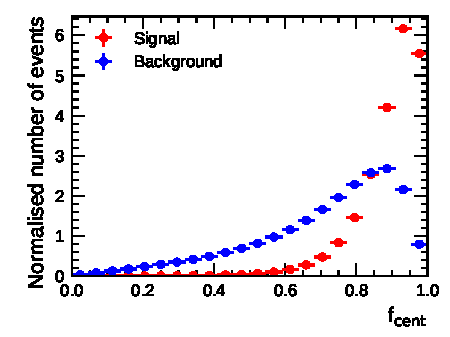
\includegraphics{./figures/baseline_bdt_vars/1p/centFrac.pdf}
  \end{subfigure}%
  \begin{subfigure}{0.5\textwidth}
    \centering
    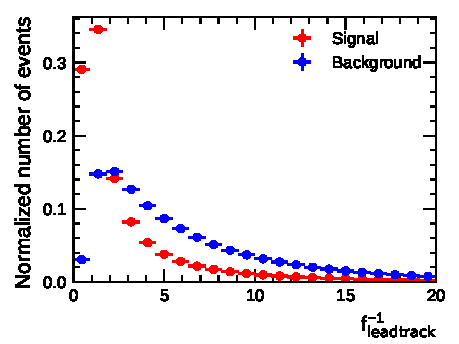
\includegraphics{./figures/baseline_bdt_vars/1p/etOverPtLeadTrk.pdf}
  \end{subfigure}
  \begin{subfigure}{0.5\textwidth}
    \centering
    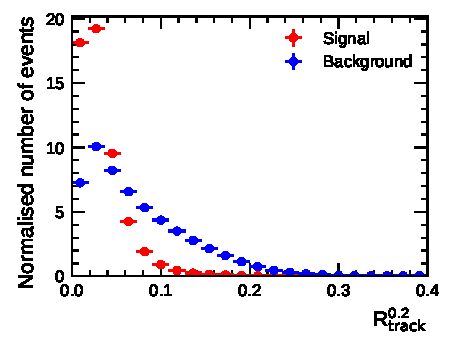
\includegraphics{./figures/baseline_bdt_vars/1p/innerTrkAvgDist.pdf}
  \end{subfigure}%
  \begin{subfigure}{0.5\textwidth}
    \centering
    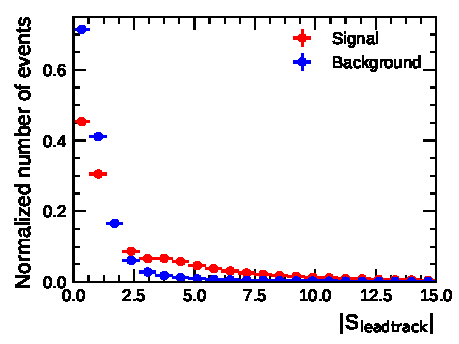
\includegraphics{./figures/baseline_bdt_vars/1p/absipSigLeadTrk.pdf}
  \end{subfigure}
  \begin{subfigure}{0.5\textwidth}
    \centering
    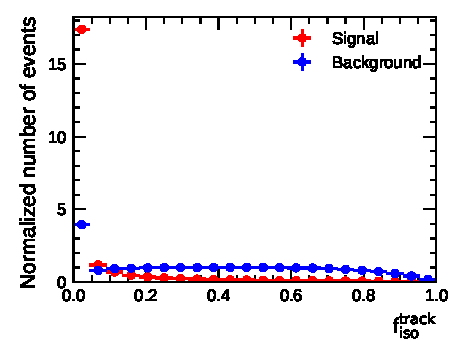
\includegraphics{./figures/baseline_bdt_vars/1p/SumPtTrkFrac.pdf}
  \end{subfigure}%
  \begin{subfigure}{0.5\textwidth}
    \centering
    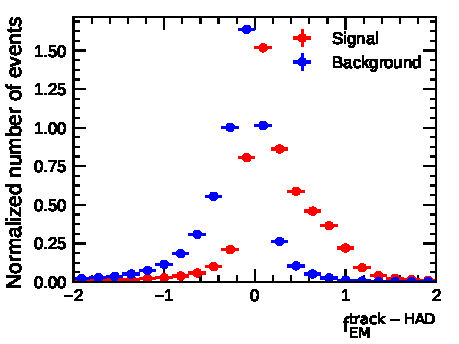
\includegraphics{./figures/baseline_bdt_vars/1p/ChPiEMEOverCaloEME.pdf}
  \end{subfigure}
  \caption{Variables used in Tau-ID BDT. \mytodo{Rename innerTrkAvgDist x-label}}
  \label{fig:bdt_vars_1p_overlays}
\end{figure}

\begin{figure}[!ht]\ContinuedFloat
  \begin{subfigure}{0.5\textwidth}
    \centering
    \includegraphics{./figures/baseline_bdt_vars/1p/EMPOverTrkSysP.pdf}
  \end{subfigure}%
  \begin{subfigure}{0.5\textwidth}
    \centering
    \includegraphics{./figures/baseline_bdt_vars/1p/ptRatioEflowApprox.pdf}
  \end{subfigure}
  \begin{subfigure}{0.5\textwidth}
    \centering
    \includegraphics{./figures/baseline_bdt_vars/1p/mEflowApprox.pdf}
  \end{subfigure}
  \caption[]{Variables used in Tau-ID BDT}
\end{figure}

\clearpage
\subsection{3-prong}

\begin{figure}[!ht]
  \begin{subfigure}{0.5\textwidth}
    \centering
    \includegraphics{./figures/baseline_bdt_vars/3p/centFrac.pdf}
  \end{subfigure}%
  \begin{subfigure}{0.5\textwidth}
    \centering
    \includegraphics{./figures/baseline_bdt_vars/3p/etOverPtLeadTrk.pdf}
  \end{subfigure}
  \begin{subfigure}{0.5\textwidth}
    \centering
    \includegraphics{./figures/baseline_bdt_vars/3p/innerTrkAvgDist.pdf}
  \end{subfigure}%
  \begin{subfigure}{0.5\textwidth}
    \centering
    \includegraphics{./figures/baseline_bdt_vars/3p/dRmax.pdf}
  \end{subfigure}
  \begin{subfigure}{0.5\textwidth}
    \centering
    \includegraphics{./figures/baseline_bdt_vars/3p/trFlightPathSig.pdf}
  \end{subfigure}%
  \begin{subfigure}{0.5\textwidth}
    \centering
    \includegraphics{./figures/baseline_bdt_vars/3p/SumPtTrkFrac.pdf}
  \end{subfigure}%
  \caption{Variables used in Tau-ID BDT\mytodo{rename innerTrkAvgDist x-label}}
  \label{fig:bdt_vars_3p_overlays}
\end{figure}

\begin{figure}[!ht]\ContinuedFloat
  \begin{subfigure}{0.5\textwidth}
    \centering
    \includegraphics{./figures/baseline_bdt_vars/3p/massTrkSys.pdf}
  \end{subfigure}%
  \begin{subfigure}{0.5\textwidth}
    \centering
    \includegraphics{./figures/baseline_bdt_vars/3p/ChPiEMEOverCaloEME.pdf}
  \end{subfigure}
  \begin{subfigure}{0.5\textwidth}
    \centering
    \includegraphics{./figures/baseline_bdt_vars/3p/EMPOverTrkSysP.pdf}
  \end{subfigure}%
  \begin{subfigure}{0.5\textwidth}
    \centering
    \includegraphics{./figures/baseline_bdt_vars/3p/ptRatioEflowApprox.pdf}
  \end{subfigure}
  \begin{subfigure}{0.5\textwidth}
    \centering
    \includegraphics{./figures/baseline_bdt_vars/3p/mEflowApprox.pdf}
  \end{subfigure}
  \caption[]{Variables used in Tau-ID BDT}
\end{figure}

\clearpage
\section{Transformed Variables}
\label{app:variable_transforms}

\begin{table}[htb]
  \centering
  \begin{tabular}{ll}
  \toprule
  Variable & Transformation \\
  \midrule
  \smash{$f_\text{cent}$} & \smash{$\min(x, 1)$} \\
  \smash{$f_\text{leadtrack}^{-1}$} & \smash{$\log(\max(0.1, x))$} \\
  \smash{$R_\text{track}$} & -- \\
  \smash{$\Delta R_\text{max}$} & -- \\
  \smash{$| S_\text{leadtrack} |$} & \smash{$\min(x, 30)$} \\
  \smash{$S_\text{T}^\text{flight}$} & \smash{$\log(\max(0.01, x))$} \\
  \bottomrule
\end{tabular}\hspace*{2em}
\begin{tabular}{ll}
  \toprule
  Variable & Transformation \\
  \midrule
  \smash{$f_\text{iso}^\text{track}$} & \smash{$\log\left(x + 10^{-4}\right)$} \\
  \smash{$f_\text{EM}^\text{track-HAD}$} & \smash{$\max(-4, \min(x, 5))$} \\
  \smash{$f_\text{track}^\text{EM}$} & \smash{$\log\left(\max\left(10^{-3}, x\right)\right)$} \\
  \smash{$p_\text{T}^\text{EM+track} / p_\text{T}$} & \smash{$\min(x, 4)$} \\
  \smash{$m_\text{EM+track}$} & \smash{$\log\left(\max(140, x / \si{\MeV})\right)$} \\
  \smash{$m_\text{track}$} & \smash{$\log\left(\max(140, x / \si{MeV})\right)$} \\
  \bottomrule
\end{tabular}


%%% Local Variables:
%%% mode: latex
%%% TeX-master: "../mythesis"
%%% End:

  \caption{Transformation applied to the input variables}
\end{table}

\clearpage
\section{TMVA-BDT Configurations}
\label{app:tmva_config}

\noindent\textbf{Common for all configurations:}\\[0.3em]
\begin{tabular}{ll}
  \texttt{NegWeightTreatment} & \texttt{IgnoreNegWeightsInTraining} \\
  \texttt{PruneMethod} & \texttt{NoPruning} \\
  \texttt{SeparationType} & \texttt{GiniIndex} \\
  \texttt{UseYesNoLeaf} & \texttt{False} \\
  \texttt{nCuts} & 200
\end{tabular}

\vfill

\noindent\textbf{Old configuration:}\\[0.3em]
\begin{tabular}{ll}
  \texttt{BoostType} & \texttt{AdaBoost} \\
  \texttt{AdaBoostBeta} & 0.2 \\
  \texttt{NTrees} & 100 \\
  \texttt{MaxDepth} & 8 \\
  \texttt{MinNodeSize} & 0.1 \\
\end{tabular}

\vfill

\noindent\textbf{1-prong (Overtrained):}\\[0.3em]
\begin{tabular}{ll}
  \texttt{BoostType} & \texttt{Grad} \\
  \texttt{Shrinkage} & 0.05 \\
  \texttt{NTrees} & 800 \\
  \texttt{MaxDepth} & 16 \\
  \texttt{MinNodeSize} & 0.01 \\
\end{tabular}

\vfill

\noindent\textbf{1-prong (cool):}\\[0.3em]
\begin{tabular}{ll}
  \texttt{BoostType} & \texttt{Grad} \\
  \texttt{Shrinkage} & 0.1 \\
  \texttt{NTrees} & 400 \\
  \texttt{UseBaggedBoost} & \texttt{True} \\
  \texttt{BaggedSampleFraction} & 0.5 \\
  \texttt{MaxDepth} & 8 \\
  \texttt{MinNodeSize} & 0.1 \\
\end{tabular}

\vfill

\noindent\textbf{3-prong (Overtrained):}\\[0.3em]
\begin{tabular}{ll}
  \texttt{BoostType} & \texttt{Grad} \\
  \texttt{Shrinkage} & 0.1 \\
  \texttt{NTrees} & 800 \\
  \texttt{MaxDepth} & 16 \\
  \texttt{MinNodeSize} & 0.01 \\
\end{tabular}

\vfill

\noindent\textbf{3-prong (cool):}\\[0.3em]
\begin{tabular}{ll}
  \texttt{BoostType} & \texttt{Grad} \\
  \texttt{Shrinkage} & 0.4 \\
  \texttt{NTrees} & 800 \\
  \texttt{MaxDepth} & 6 \\
  \texttt{MinNodeSize} & 0.1 \\
\end{tabular}

\clearpage
\section{Decay Mode Classification using Recurrent Neural Networks}
\subsection{Baseline Probabilities}
\label{app:baseline_probabilities}

\begin{figure}[!ht]
  \begin{subfigure}{0.48\textwidth}
    \centering
    \includegraphics{./figures/decay_mode_classification/mode_proba_baseline_ptcut_1_5/proba_1p0n.pdf}
  \end{subfigure}\hfill
  \begin{subfigure}{0.48\textwidth}
    \centering
    \includegraphics{./figures/decay_mode_classification/mode_proba_baseline_ptcut_1_5/proba_1p1n.pdf}
  \end{subfigure}
  \begin{subfigure}{0.48\textwidth}
    \centering
    \includegraphics{./figures/decay_mode_classification/mode_proba_baseline_ptcut_1_5/proba_1pXn.pdf}
  \end{subfigure}\hfill
  \begin{subfigure}{0.48\textwidth}
    \centering
    \includegraphics{./figures/decay_mode_classification/mode_proba_baseline_ptcut_1_5/proba_3p0n.pdf}
  \end{subfigure}
  \begin{subfigure}{0.48\textwidth}
    \centering
    \includegraphics{./figures/decay_mode_classification/mode_proba_baseline_ptcut_1_5/proba_3pXn.pdf}
  \end{subfigure}%

  \caption{Multi-class probabilities for the Baseline RNN}
  \label{fig:rnn_multiclass_proba_baseline}
\end{figure}

\clearpage
\subsection{Combined Probabilities}
\label{app:combined_probabilities}

\begin{figure}[!ht]
  \begin{subfigure}{0.48\textwidth}
    \centering
    \includegraphics{./figures/decay_mode_classification/combined_proba/proba_1p0n.pdf}
  \end{subfigure}\hfill
  \begin{subfigure}{0.48\textwidth}
    \centering
    \includegraphics{./figures/decay_mode_classification/combined_proba/proba_1p1n.pdf}
  \end{subfigure}
  \begin{subfigure}{0.48\textwidth}
    \centering
    \includegraphics{./figures/decay_mode_classification/combined_proba/proba_1pXn.pdf}
  \end{subfigure}\hfill
  \begin{subfigure}{0.48\textwidth}
    \centering
    \includegraphics{./figures/decay_mode_classification/combined_proba/proba_3p0n.pdf}
  \end{subfigure}
  \begin{subfigure}{0.48\textwidth}
    \centering
    \includegraphics{./figures/decay_mode_classification/combined_proba/proba_3pXn.pdf}
  \end{subfigure}%

  \caption{Multi-class probabilities for the Combined RNN}
  \label{fig:rnn_multiclass_proba_combined}
\end{figure}

\clearpage
\section{Grid Search: 3-Prong}
\label{app:grid_search_3p}

\begin{figure}[htbp]
  \begin{subfigure}[t]{0.48\textwidth}
    \centering
    \includegraphics{./figures/bdt_perf/gridsearch_3p/scan_MaxDepth_NTrees.pdf}
    \subcaption{}
  \end{subfigure}\hfill
  \begin{subfigure}[t]{0.48\textwidth}
    \centering
    \includegraphics{./figures/bdt_perf/gridsearch_3p/scan_Shrinkage_NTrees.pdf}
    \subcaption{}
  \end{subfigure}
  \begin{subfigure}[t]{0.48\textwidth}
    \centering
    \includegraphics{./figures/bdt_perf/gridsearch_3p/scan_Shrinkage_MaxDepth.pdf}
    \subcaption{}
  \end{subfigure}\hfill
  \begin{subfigure}[t]{0.48\textwidth}
    \centering
    \includegraphics{./figures/bdt_perf/gridsearch_3p/scan_MinNodeSize_MaxDepth.pdf}
    \subcaption{}
  \end{subfigure}
  \caption{Background rejection at \SI{60}{\percent} signal efficiency as a
    function of the BDT hyperparameters. Bagged boosting with a subsample
    fraction~$f_\text{bag} = \SI{50}{\percent}$ is used and the remaining
    parameters are fixed such that the 'best' BDT is contained within the
    plots.}
  \todo[inline]{Better word for 'best' as it is not the best BDT}
  \label{fig:hyperparameter_scan_3p}
\end{figure}

\clearpage
\section{BDT: Recursive Feature Elimination}

\begin{figure}[htb]
  \centering
  \begin{subfigure}[t]{0.33\textwidth}
    \centering
    \includegraphics{./figures/bdt_perf/var_importance/1p_iter1.pdf}
    \subcaption{Iteration 1}
  \end{subfigure}
  \begin{subfigure}[t]{0.33\textwidth}
    \centering
    \includegraphics{./figures/bdt_perf/var_importance/1p_iter2.pdf}
    \subcaption{Iteration 2}
  \end{subfigure}
  \caption{Variable importance (1-prong). Averaged rejection loss over a
    gamma-tautau like dijet spectrum. Tight working point.}
  \label{fig:variable_importance_1p_app}
\end{figure}

\begin{figure}[htb]
  \centering
  \begin{subfigure}[t]{0.32\textwidth}
    \centering
    \includegraphics{./figures/bdt_perf/var_importance/3p_iter1.pdf}
    \subcaption{Iteration 1}
  \end{subfigure}
  \begin{subfigure}[t]{0.32\textwidth}
    \centering
    \includegraphics{./figures/bdt_perf/var_importance/3p_iter2.pdf}
    \subcaption{Iteration 2}
  \end{subfigure}
  \begin{subfigure}[t]{0.32\textwidth}
    \centering
    \includegraphics{./figures/bdt_perf/var_importance/3p_iter3.pdf}
    \subcaption{Iteration 3}
  \end{subfigure}

  \caption{Variable importance (3-prong). Averaged rejection loss over a
    gamma-tautau like dijet spectrum. Tight working point.}
  \label{fig:variable_importance_3p_app}
\end{figure}

\clearpage
\section{Post-Optimisation Working Points}

\begin{figure}[htb]
  \centering
  \begin{subfigure}{0.48\textwidth}
    \centering
    \includegraphics{./figures/bdt_perf/post_optimisation/rejection_medium_1p.pdf}
  \end{subfigure}\hfill
  \begin{subfigure}{0.48\textwidth}
    \centering
    \includegraphics{./figures/bdt_perf/post_optimisation/rejection_loose_1p.pdf}
  \end{subfigure}
  \caption{1-prong}
\end{figure}

\begin{figure}[htb]
  \centering
  \begin{subfigure}{0.48\textwidth}
    \centering
    \includegraphics{./figures/bdt_perf/post_optimisation/rejection_medium_3p.pdf}
  \end{subfigure}\hfill
  \begin{subfigure}{0.48\textwidth}
    \centering
    \includegraphics{./figures/bdt_perf/post_optimisation/rejection_loose_3p.pdf}
  \end{subfigure}
  \caption{3-prong}
\end{figure}

\clearpage
\section{Rejection vs.\ Initiating Parton}
\begin{figure}[htb]
  \centering
  \begin{subfigure}[t]{0.48\textwidth}
    \centering
    \includegraphics{./figures/bdt_perf/parton/truth_parton_1p.pdf}
    \caption{1-prong}
  \end{subfigure}\hfill
  \begin{subfigure}[t]{0.48\textwidth}
    \centering
    \includegraphics{./figures/bdt_perf/parton/truth_parton_3p.pdf}
    \caption{3-prong. Loose working point (Tight has too much rejection for
      limited stats)}
  \end{subfigure}
  \caption{Rejection vs initiating parton}
\end{figure}

\todo[inline]{Due to the longer decay chain of B-hadrons, the number of
  particles and angular spread is larger for a b-jet than a light-quark jet.}

\clearpage
\section{Decay Mode Classification Experiments}
\label{sec:app_decay_mode_exp}
\begin{figure}[htb]
  \begin{subfigure}[t]{0.48\textwidth}
    \centering
    \includegraphics{./figures/decay_mode_classification/experiments/mig_mat_conversions.pdf}
    \subcaption{Migration matrix}
  \end{subfigure}\hfill
  \begin{subfigure}[t]{0.48\textwidth}
    \centering
    \includegraphics{./figures/decay_mode_classification/experiments/comp_mat_conversions.pdf}
    \subcaption{Composition matrix}
  \end{subfigure}
  \caption{Conversion tracks}
\end{figure}

\begin{figure}[htb]
  \begin{subfigure}[t]{0.48\textwidth}
    \centering
    \includegraphics{./figures/decay_mode_classification/experiments/mig_mat_shots.pdf}
    \subcaption{Migration matrix}
  \end{subfigure}\hfill
  \begin{subfigure}[t]{0.48\textwidth}
    \centering
    \includegraphics{./figures/decay_mode_classification/experiments/comp_mat_shots.pdf}
    \subcaption{Composition matrix}
  \end{subfigure}
  \caption{Shots}
\end{figure}

\begin{figure}[htb]
  \begin{subfigure}[t]{0.48\textwidth}
    \centering
    \includegraphics{./figures/decay_mode_classification/experiments/mig_mat_moments.pdf}
    \subcaption{Migration matrix}
  \end{subfigure}\hfill
  \begin{subfigure}[t]{0.48\textwidth}
    \centering
    \includegraphics{./figures/decay_mode_classification/experiments/comp_mat_moments.pdf}
    \subcaption{Composition matrix}
  \end{subfigure}
  \caption{Add.\ cluster moments}
\end{figure}

\begin{figure}[htb]
  \begin{subfigure}[t]{0.48\textwidth}
    \centering
    \includegraphics{./figures/decay_mode_classification/experiments/mig_mat_hadronic_pfos.pdf}
    \subcaption{Migration matrix}
  \end{subfigure}\hfill
  \begin{subfigure}[t]{0.48\textwidth}
    \centering
    \includegraphics{./figures/decay_mode_classification/experiments/comp_mat_hadronic_pfos.pdf}
    \subcaption{Composition matrix}
  \end{subfigure}
  \caption{Hadronic PFOs}
\end{figure}

\begin{figure}[htb]
  \begin{subfigure}[t]{0.48\textwidth}
    \centering
    \includegraphics{./figures/decay_mode_classification/experiments/mig_mat_sub_e_2.pdf}
    \subcaption{Migration matrix}
  \end{subfigure}\hfill
  \begin{subfigure}[t]{0.48\textwidth}
    \centering
    \includegraphics{./figures/decay_mode_classification/experiments/comp_mat_sub_e_2.pdf}
    \subcaption{Composition matrix}
  \end{subfigure}
  \caption{$p_\text{T}$-fraction}
\end{figure}

\clearpage
\section{Combined After Tau-ID}

\begin{figure}[htbp]
  \begin{subfigure}{0.48\textwidth}
    \centering
    \includegraphics{./figures/decay_mode_classification/combined_sub_e_moments_shots_conv_ptcut_1_5/mig_mat_med_id.pdf}
    \subcaption{Migration matrix}
  \end{subfigure}\hfill
  \begin{subfigure}{0.48\textwidth}
    \centering
    \includegraphics{./figures/decay_mode_classification/combined_sub_e_moments_shots_conv_ptcut_1_5/comp_mat_med_id.pdf}
    \subcaption{ Purity matrix}
  \end{subfigure}
  \caption{Combined with medium tau id}
  \label{fig:decay_mode_combined_med_id}
\end{figure}

\clearpage
\section{Track-Constrained Decay Mode Classification}
\label{app:mode_classification_track_constraint}

\begin{figure}[htbp]
  \begin{subfigure}{0.48\textwidth}
    \centering
    \includegraphics{./figures/decay_mode_classification/combined_sub_e_moments_shots_conv_ptcut_1_5/mig_mat.pdf}
    \subcaption{Extended model without track constraint.}
  \end{subfigure}\hfill
  \begin{subfigure}{0.48\textwidth}
    \centering
    \includegraphics{./figures/decay_mode_classification/combined_sub_e_moments_shots_conv_ptcut_1_5/mig_mat_use_ntracks.pdf}
    \subcaption{Extended model with track constraint.}
  \end{subfigure}
  \caption{Migration matrix for the extended model including conversion, shot
    and additional cluster information. The model is constrained by setting
    estimated mode probabilities to zero for modes not consistent with the
    number of reconstructed tracks.}
\end{figure}

\clearpage
\section{High-$p_\text{T}$}
\label{sec:combined_high_pt_migration}

\begin{figure}[htb]
    \begin{subfigure}{0.48\textwidth}
    \centering
    \includegraphics{./figures/decay_mode_classification/highpt/mig_mat_pt_less_100.pdf}
    \subcaption{Migration matrix. $p_\text{T} < \SI{100}{\giga\electronvolt}$}
  \end{subfigure}\hfill
  \begin{subfigure}{0.48\textwidth}
    \centering
    \includegraphics{./figures/decay_mode_classification/highpt/comp_mat_pt_less_100.pdf}
    \subcaption{Migration matrix. $p_\text{T} < \SI{100}{\giga\electronvolt}$}
  \end{subfigure}
  \begin{subfigure}{0.48\textwidth}
    \centering
    \includegraphics{./figures/decay_mode_classification/highpt/mig_mat_pt_geq_100.pdf}
    \subcaption{Migration matrix. $p_\text{T} > \SI{100}{\giga\electronvolt}$}
  \end{subfigure}\hfill
  \begin{subfigure}{0.48\textwidth}
    \centering
    \includegraphics{./figures/decay_mode_classification/highpt/comp_mat_geq_100.pdf}
    \subcaption{Purity matrix. $p_\text{T} > \SI{100}{\giga\electronvolt}$}
  \end{subfigure}
  \caption{highpt}
  \label{fig:highpt_matrices}
\end{figure}

\clearpage
\section{TODOS}
\listoftodos

%%% Local Variables:
%%% mode: latex
%%% TeX-master: "mythesis"
%%% End:

% \printbibliography[heading=subbibliography]

%------------------------------------------------------------------------------
% Declare lists of figures and tables and acknowledgements as backmatter
% Chapter/section numbers are turned off
\backmatter

\listoffigures
\listoftables

%------------------------------------------------------------------------------
% Print the glossary and list of acronyms
% \printglossaries

%------------------------------------------------------------------------------
% You could instead add your acknowledgements here - don't forget to
% also add them to \includeonly above
%------------------------------------------------------------------------------
\chapter{Acknowledgements}
\label{sec:ack}
%------------------------------------------------------------------------------

This thesis would not have been possible without the help, guidance and support
of many people. Therefore, I would like to thank:
\begin{itemize}
\item Prof.\ Dr.\ Jochen Dingfelder for giving me the opportunity to write my
  thesis in his working group and for his continued support.

\item Prof.\ Dr.\ Klaus Desch for his willingness to co-examine my thesis.

\item Dr.\ William Davey for his excellent supervision, guidance and the many
  fruitful discussions.

\item Benedict Winter for his valuable advice and him sharing his vast
  knowledge of physics with me.

\item My (past) office colleagues Verena Muckhoff, Jan Heinrichs, and Christos
  Vergis for the enjoyable office atmosphere.

\item All of my colleagues in the working group of Prof.\ Dingfelder.

\item My family for providing me with support and stability during my studies.

\end{itemize}



%%% Local Variables:
%%% mode: latex
%%% TeX-master: "mythesis"
%%% End:


%------------------------------------------------------------------------------
% CV needed when you submit your PhD thesis
% \definecolor{lightgray}{gray}{0.8}
\newcolumntype{L}{>{\raggedleft}p{0.15\textwidth}}
\newcolumntype{R}{p{0.8\textwidth}}
\newcommand\VRule{\color{lightgray}\vrule width 0.5pt}

\thispagestyle{empty}
\section*{Curriculum Vitae}

\subsection*{Personal Details}

\begin{tabular}{L!{\VRule}R}
Name & Johann Schmidt \\
Date of Birth &  \\
Email & abc@physik.uni-def.de \\
Family status & Single
\end{tabular}

\subsection*{Education}

\begin{tabular}{L!{\VRule}R}
1997--2003 & Abitur, ABC Secondary School, Hamburg, Germany\\
2004--2007 & BSc in Physics, Rheinische Friedrich-Wilhelms-Universität, Bonn, Germany.\\
2006 & CERN Summer Student, Geneva, Switzerland. \\
2007--2009 &  MSc in Physics Rheinische Friedrich-Wilhelms-Universität, Bonn, Germany. \\
2009--2012 &  PhD in Physics, Rheinische Friedrich-Wilhelms-Universität, Bonn, Germany. \\
2012 & Advanced Data Analysis School, Frankfurt, Germany.
\end{tabular}

\subsection*{Professional Experience}

\begin{tabular}{L!{\VRule}R}
2004 & Summer Student at CERN, Geneva, Switzerland. \\
2007--2012 & Doctoral work at the University of Bonn, Germany. \\
2008--2009 & Fieldwork at CERN, Geneva, Switzerland.\\
2011 & Talk at the Advanced Physics Conference, Timbucto
\end{tabular}

\subsection*{Languages}
\begin{tabular}{L!{\VRule}R}
German & Mother tongue \\
English & Fluent \\
Russian & Basic
\end{tabular}


\end{document}

%%% Local Variables:
%%% mode: latex
%%% TeX-master: t
%%% End:
